\documentclass{scrartcl}
%%%%%%%%%%%%%%%%%%%%%%%%%%%%%%%%%%%%%%%%%%%%%%%%%%%%%%%%%%%%%%%%%%%%%%%%%%%%%%%%%%%%%%%%%%%%%%%%%%%%%%%%%%%%%%%%%%%%%%%%%%%%%%%%%%%%%%%%%%%%%%%%%%%%%%%%%%%%%%%%%%%%%%%%%%%%%%%%%%%%%%%%%%%%%%%%%%%%%%%%%%%%%%%%%%%%%%%%%%%%%%%%%%%%%%%%%%%%%%%%%%%%%%%%%%%%
\usepackage[ngerman]{babel}
\usepackage[utf8]{inputenc}
\usepackage[T1]{fontenc}
\usepackage{ae,aecompl}
\usepackage[a4paper,bottom=1in,top=1in]{geometry}
\usepackage{amssymb,amsmath,amsfonts}
\usepackage{csquotes}
\usepackage{pdfsync}
\usepackage{enumerate}
\usepackage{graphicx}
\usepackage{qtree}
\usepackage{pdfpages}
\usepackage{hyperref}
\hypersetup{
pdfauthor={Willi Mutschler},
pdftitle={Makro Anschrift A},
pdfsubject={},
pdfproducer={LaTeX},
colorlinks=false,  pdfborder={0 0 0},     pdfstartview={FitH},   plainpages = false, }
\usepackage{fancyhdr}
\pagestyle{fancy}
\lhead{\small Makro\"{o}konomik Anschrift A (Willi Mutschler)}

\begin{document}

\section*{TO DO}
\begin{itemize}
  \item A0: Vorbemerkungen
  \item Rechenaufgabe Klassik Fehler
  \item A3.1:
  \begin{itemize}
    \item Unterschiede zur Klassik genauer
    \item Sparparadox
    \item Sparfunktion umgedrehte Grafik
    \item Erl\"{a}uterungen verbessern
    \item Erl\"{a}uterungen Keynes Kreuz
    \item Passt $Y_s$,$Y_d$,$Y$ bei Multiplikator Schaubild?
    \item Erl\"{a}uterung Treppe
  \end{itemize}
  \item A3.2: Investitionsnachfrage besser
  \item A3.3: Geldnachfrage Motive sauberer
  \item A5: Hicksche Wachstumsmodell Idee sauberer, warum Akzelerator?
  \item L\"{o}sungen zu A6.3, A6.4, A7.1, A7.2, A8 Solow, A9 Phillips.
\end{itemize}
\section{VGR}
\subsection{Verst\"{a}ndnis}
\begin{itemize}
\item Prinzip: Wie gro{\ss} ist der Kuchen? H\"{o}he des Bruttoinlandsprodukts!
\item Entstehung: Wodurch wurde der Kuchen generiert?\\ Gesamte Wertsch\"{o}pfung, Summe aller Mehrwerte
\item Verwendung: Was wird mit den Kuchenst\"{u}cken gemacht?\\ Konsum, Ersparnis, Investitionen, Exporte, Importe
\item Verteilung: Wer erh\"{a}lt etwas vom Kuchen?\\ Volkseinkommen: L\"{o}hne, Gewinne
\item Vokabular:
    \begin{itemize}
      \item Stromgr\"{o}{\ss}en: Einkommen, Konsum, Investitionen, Abschreibungen, Gewinn, Geburten, Sterbef\"{a}lle\\ (\emph{pro} Periode, \textbf{Zeitraumbezogen})
      \item Bestandsgr\"{o}{\ss}en: Verm\"{o}gen, Kapitalstock, Bev\"{o}lkerungszahl, Arbeitslosigkeit, Geldmenge\\ (\emph{in} Periode, \textbf{Zeitpunktbezogen})
    \end{itemize}
\item Sektoren/Akteure
    \begin{itemize}
      \item Haushalte: erbringen Faktorleistungen, konsumieren und sparen
      \item Unternehmen: produzieren und verkaufen Waren und Dienstleistungen, zahlen L\"{o}hne und Gewinne, investieren und verschulden sich
      \item Staat: Staatskonsum, Staatsinvestitionen, Steuern, Subventionen, Transfers
      \item Ausland (\"{u}brige Welt): Export/Import von Waren, Dienst- und Faktorleistungen
    \end{itemize}
\item Wichtigstes Prinzip: Angebot $=$ Nachfrage:
    \begin{align*}
      \underbrace{Y+IM}_\text{Angebot} &= \underbrace{C+I+G+EX}_\text{Nachfrage}
    \end{align*}
    Zentraler Unterschied offene vs. geschlossene Volkswirtschaft:\\
    Gesamtwirtschaftliche inl\"{a}ndische Nachfrage muss nicht gleich dem inl\"{a}ndischem Angebot an G\"{u}tern und Dienstleistungen sein! G\"{u}ter k\"{o}nnen vom Ausland importiert bzw. ins Ausland exportiert werden. Kapitalimporte: Kauf von inl\"{a}ndischen Wertpapieren durch Ausl\"{a}nder. Kapitalexporte: Kauf von ausl\"{a}ndischen Wertpapieren durch Inl\"{a}nder. Zahlungsbilanz erfasst alle Transaktionen zwischen Inl\"{a}ndern und Ausl\"{a}ndern. Wir betrachten also folgenden Au{\ss}enbeitrag und Finanzierungssaldo
    \begin{multline*}
      AB = \underbrace{EX-IM}_\text{Nettoexporte} = \\
      \underbrace{(Y - C_{Pr} - T)}_{S_{Pr}} + \underbrace{(T-C_{St})}_{S_{St}} - I_{Pr} - I_{St}=\\ \underbrace{S-I}_\text{Nettokapitalablfl\"{u}sse} =FS_{Inland} = -FS_{UW}
    \end{multline*}
    Hinweis: Formel $FS= Sparen-Investitionen = Einnahmen - Ausgaben$ ist immer Finanzierungssaldo, entweder f\"{u}r Volkswirtschaft gesamt oder einzelne Akteure.
    \begin{itemize}
      \item $EX-IM$ ist internationaler G\"{u}terstrom, $S-I$ ist internationaler Finanzstrom
      \item $EX>IM$ Leistungsbilanz\"{u}berschuss, $S>I$ Nettodarlehensgeber
      \item $EX<IM$ Leistungsbilanzdefizit, $S<I$ Nettodarlehensnehmer
    \end{itemize}
    Ein Leistungsbilanz-Defizit erfordert einen Kapitalzufluss zur Finanzierung der Nettoimporte!
\item Was h\"{a}ngt wie zusammen?
    \begin{align*}
    &\text{\textbf{Entstehungsrechnung}:}\\
      BIP&= \overbrace{\underbrace{PW}_\text{Produktionswert} - \underbrace{V}_\text{Vorleistungen}}^\text{Bruttowertsch\"{o}pfung} + \underbrace{T_G}_\text{G\"{u}tersteuern} - \underbrace{SUB_G}_\text{G\"{u}tersubventionen} \\
    &\text{\textbf{Verwendungsrechnung}:}\\
      BIP &= (C_{pr} + C_{St}) + (I_{br,pr}+I_{br,St}) + EX-IM \qquad \Rightarrow \text{FOKUS INLAND}\\
      BNE &= BIP +  \underbrace{\text{Saldo Prim\"{a}reinkommen Welt}}_{+\text{EK Inl\"{a}nder im Ausland}-\text{EK Ausl\"{a}nder im Inland}} \qquad \Rightarrow \text{FOKUS INL\"{A}NDER}\\
      NNE &= BNE - ABS\\
&\text{\textbf{Verteilungsrechnung}:}\\
      \underbrace{Y}_\text{Volkseinkommen} &= NNE - \underbrace{\underbrace{T_{ind}}_\text{ind. Steuern}}_{Mehrwertsteuer, Okosteuer, Alkohol, Tabak, Gewerbe, Strom} + \underbrace{SUB}_\text{Unt-Subventionen}\\
      \underbrace{Y}_\text{Volkseinkommen} & = \underbrace{W}_\text{ANEntgelt} + \underbrace{Q}_\text{Untern.undVerm\"{o}gens.EK}\\
      \underbrace{YV}_\text{Verf\"{u}gbares EK} &= NNE + \underbrace{SLU}_\text{Saldo lauf. \"{U}bertragungen (+aus \"{U}W -in \"{U}W)}\\
      \underbrace{YV}_\text{Verf\"{u}gbares EK}  &= YV_{Pr} + YV_{St} = C_{Pr} + S_{Pr} + C_{St} + S_{St} = C + S
    \end{align*}
\item Wichtige Konzepte:
    \begin{itemize}
        \item Inlandskonzept: Produktion innerhalb Grenzen, unabh\"{a}ngig von wem ($\hookrightarrow$ BIP)
        \item Inl\"{a}nderkonzept: Durch Inl\"{a}nder get\"{a}tigte Produktion bzw. erzieltes Einkommen, unabh\"{a}ngig ob im Inland oder Ausland ($\hookrightarrow$ BNE)
        \item Abschreibungen: Netto = Brutto - ABS, au{\ss}er Nettol\"{o}hne = Bruttol\"{o}hne-$T_{dir,W}$ und Nettogewinne = Bruttogewinne-$T_{dir,Q}$
      \end{itemize}
\end{itemize}
\subsection{Einfache Berechnungen}
\begin{align*}
  BIP &= PW - V + T_G - SUB_G = 5000 - 2700 + 580 - 30 = 2850\\
  LB &= EX - IM = BIP - C_{Pr} - C_{St} - I_{Br} = 2850 - 1000 - 500 - 870 = 480\\
  EX &= LB + IM = 480 + 770 = 1250\\
  I_{netto} &= I_{Br} - ABS = 870-450=420\\
  BNE &= BIP + Saldo PEK = 2850 - 40 = 2810\\
  NNE &= BNE - ABS = 2810 - 450 = 2360
\end{align*}

\subsection{Berechnungen (I)}
\begin{align*}
  Y &= NNE - T_{ind} + SUB \\&= BNE-ABS - T_{ind} + SUB \\&= BIP + SPEK - ABS - T_{ind} + SUB \\&= C+ I_{br}+\underbrace{EX-IM}_{AB} + SPEK - ABS - T_{ind} + SUB\\
  \Leftrightarrow I_{br} &= Y-C-AB-SPEK+ABS+T_{ind}-SUB
\end{align*}

\subsection{Berechnungen (II)}
\begin{align*}
  NNE &= YV - SLU \\&=YV_{Pr} + YV_{St} - SLU \\&= YV_{Pr}+ C_{St} + S_{St} - SLU \\&= YV_{Pr}+ C- C_{Pr} + S_{St} - SLU
\end{align*}

\subsection{Berechnungen (III)}
\begin{align*}
  PW &= BIP + V-T_G + SUB_G \\&= BNE-SPEK+V-T_G+Sub_G
\end{align*}

\subsection{Berechnungen (IV)}
\begin{align*}
  YV &= NNE+SLU \\&=BNE-ABS+SLU\\&=BIP+SPEK-ABS+SLU\\&=C+I+\underbrace{EX-IM}_{AB}+SPEK-ABS+SLU\\
  \Leftrightarrow I &= YV-C-AB-SPEK+ABS-SLU
\end{align*}
mit SPEK = EK Inl\"{a}nder im Ausland - Ausl\"{a}nder im Inland und SLU = LU aus \"{U}W - LU in \"{U}W.


\subsection{Kreislaufschema (I)}
Wichtig: Summe aller eingehenden Pfeile muss in jedem Block immer gleich der Summe aller ausgehenden Pfeile sein! Es gilt also:
\begin{align*}
  UW:& IM=EX+FS_{UW}\\
  HH:& W+Q = FS_{HH} + C_{Pr} + T_{dir}\\
  ST:& T_{dir} = FS_{St} + I_{St} \\
  U:& I_{St} + C_{Pr} + Ex + I_{Pr} = FS_{U} + W+Q + IM + I_{Pr}\\
  FM:& FS_{UW} + FS_{HH} + FS_{St} + FS_{U} = 0
\end{align*}
Es gilt: $Y=W+Q$. Weiterhin gilt $FS_U=-I_{Pr}$, da aus U folgt:
\begin{align*}
-FS_U = \underbrace{W+Q}_Y - EX + IM - C_{Pr} - I_{St}
\end{align*}
und
\begin{align*}
Y=C_{Pr}+C_{St}+I_{Pr}+I_{St}+EX-IM\\
\Leftrightarrow Y-EX+IM-C_{Pr}-C_{St}-I_{St} = I_{Pr}
\end{align*}
Somit $-FS_U = I_{Pr}$, da hier $C_{St}=0$. Also:
\begin{align*}
  &Y=W+Q=140\\
  &FS_U = - I_{Pr} = -10\\
  UW:& FS_{UW} = IM-EX = -30\\
  FM:& FS_{St} = - (FS_{UW}+FS_{HH}+FS_U) = 20\\
  ST:& T_{dir} = I_{St} + FS_{St} = 50\\
  HH:& C_{Pr} = W+Q - FS_{HH}-T_{dir} = 70
\end{align*}


\subsection{Kreislaufschema (II)}
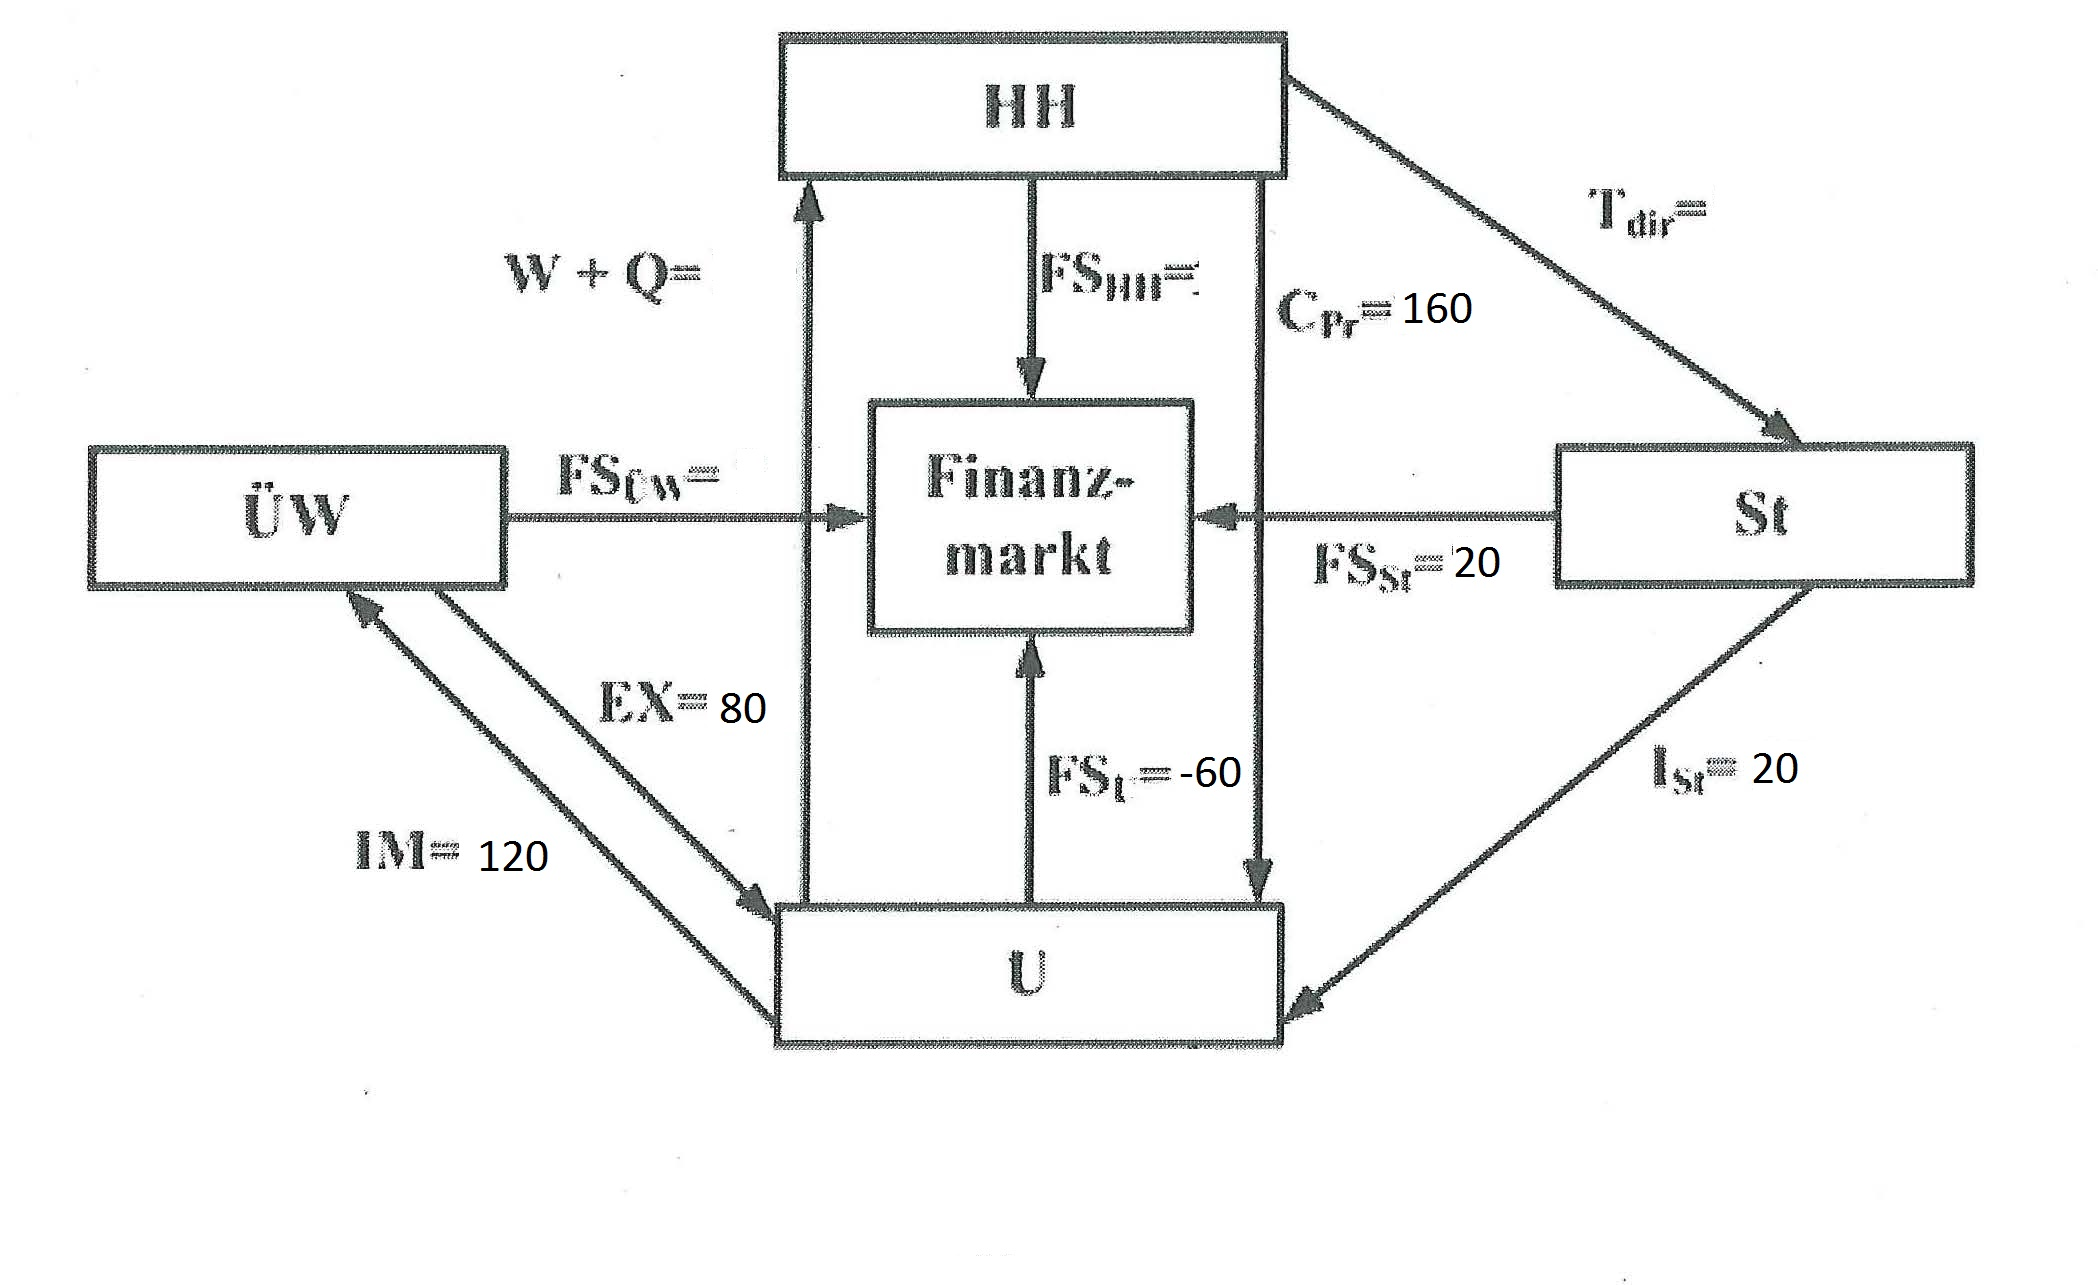
\includegraphics[width=\textwidth]{Bilder/Klassik_Kreislauf_Diagramm_Anschrift.jpg}
Wichtig: Summe aller eingehenden Pfeile muss in jedem Block immer gleich der Summe aller ausgehenden Pfeile sein! Es gilt also:
\begin{align*}
  UW:& IM=EX+FS_{UW}\\
  HH:& W+Q = FS_{HH} + C_{Pr} + T_{dir}\\
  ST:& T_{dir} = FS_{St} + I_{St} \\
  U:& I_{St} + C_{Pr} + Ex + I_{Pr} = FS_{U} + W+Q + IM + I_{Pr}\\
  FM:& FS_{UW} + FS_{HH} + FS_{St} + FS_{U} = 0
\end{align*}
Also:
\begin{align*}
  UW:& FS_{UW} = IM-EX = 40\\
  FM:& FS_{HH} = - (FS_{UW}+FS_{ST}+FS_U) = 0\\
  ST:& T_{dir} = I_{St} + FS_{St} = 40\\
  HH:& W+Q = C_{Pr} + FS_{HH} + T_{dir}  = 200
\end{align*}

\subsection{Finanzierungssalden}
\begin{enumerate}
  \item F\"{u}r jeden Sektor gilt: Finanzierungssaldo = Sparen - Investitionen bzw. Einnahmen - Ausgaben.
  \begin{itemize}
  \item F\"{u}r Haushalte: $FS_H=S_{Pr}-0 = YV_{Pr}-C_{Pr} = Y-T_{dir}+TR-C_{Pr}$
  \item F\"{u}r Unternehmen: $FS_U=0-I_{Pr} = -I_{Pr}$
  \item F\"{u}r Staat: $FS_{St} = S_{St} - I_{St} = T_{dir}-TR - C_{St} - I_{St}$
  \end{itemize}
  \item Die Summe der Finanzierungssalden aller Sektoren erg\"{a}nzt sich immer zu Null, da gesamtwirtschaftlich jeder Forderung in gleicher H\"{o}he eine Verbindlichkeit gegen\"{u}bersteht.
\end{enumerate}

\subsection{Geschlossene vs. Offene Volkswirtschaft}
\begin{align*}
  Y &= NNE - T_{ind} + SUB = BNE-ABS-T_{ind}+SUB = BIP + SPEK - ABS - T_{ind} + SUB
\end{align*}
und
\begin{align*}
  Y &=C_{Pr}+C_{St} + I_{Pr}+I_{St} + EX - IM + SPEK - ABS - T_{ind} + SUB
\end{align*}
  \begin{enumerate}
    \item Hier: $C_{St}= G$, $I_{St}=0$, $EX=IM=0$, $SPEK=0$, $ABS=0$, $T_{ind}=0$, $SUB=0$, also: $Y=BIP$
    \item Budgetdefizit: $BD=-FS_U=-(S_{St}-I_{St})$. Mit
    \begin{align*}
      S-I=0\\
      \Leftrightarrow S_{Pr}-I_{Pr} + S_{St}-I_{St} = 0\\
      \Leftrightarrow S_{Pr} = I_{Pr} - (S_{St}-I_{St}) = I_{Pr}+BD
    \end{align*}
    Ersparnis der privaten Haushalte muss private Investitionen und Staatsdefizit finanzieren.
    \item Budgetdefizit: $BD=-FS_U=-(S_{St}-I_{St})$. Mit
    \begin{align*}
      S-I=EX-IM=AB\\
      \Leftrightarrow S_{Pr}-I_{Pr} + S_{St}-I_{St} = AB\\
      \Leftrightarrow S_{Pr} = I_{Pr} - (S_{St}-I_{St}) + AB = I_{Pr}+BD+AB
    \end{align*}
    Ersparnis der privaten Haushalte muss private Investitionen, Au{\ss}enbeitrag und Staatsdefizit finanzieren.
  \end{enumerate}

\subsection{Verst\"{a}ndnisfragen (15 Min)}
\begin{enumerate}
  \item $NNE=BNE - ABS$ (wahr)
  \item $S=Y-C$ alles Stromgr\"{o}{\ss}en! (falsch)
  \item $S-I_{br} =S-(I_{net}+ABS)= EX-IM$ kann alles sein (wahr)
  \item $NWS = BWS -ABS, ABS>NWS, BWS = NWS + AB >0$ (falsch)
  \item Dies ist die Definition (wahr)
  \item Geschlossene Volkswirtschaft: $S=I$ Finanzierungssaldo: $FS=S-I = 0$ (wahr)\\
  Warum Finanzierung: $S_H + S_U + S_{St} = I_{U}+I_{St} \Leftrightarrow S_H + (S_U-I_U)+(S_{St}-I_{St})$
  \item $NIP = BIP-ABS, NNE = BIP + SPEK -ABS,\\ NNE < NIP \Leftrightarrow BIP +SPEK - ABS < BIP -ABS \Leftrightarrow SPEK < 0 \rightarrow $ m\"{o}glich! (falsch)
  \item $YV = NNE + SLU$ (falsch)
  \item falsch.
  \item $NNE=BIP+SPEK-ABS, NNE-BIP<0 \leftrightarrow SPEK < ABS$ m\"{o}glich! (falsch)
  \item Verteilung des \textbf{EINKOMMENS} auf L\"{o}hne und Gewinne! (falsch)
  \item $I_{netto} = I_{br} - ABS$. Wenn Bruttoinvestitionen unterbleiben und gleichzeitig der Kapitalbestand an Wert verliert, ist $I_{netto}<0$ m\"{o}glich. Die Bruttoinvestition ist entweder positiv oder gleich Null, denn eine Volkswirtschaft kann nicht weniger als nichts investieren! (falsch)
  \item $S-I<0$, es muss Kapital importiert werden um Investitionen zu finanzieren (wahr)
  \item $S-I^{br} = S - I^{ne} -ABS$, f\"{u}r ABS=0 gilt $S=I^{ne}$ (wahr)
  \item $I_{br} = I_{netto} + ABS, I_{br} > ABS \leftrightarrow I_{netto} > 0$ (falsch)
  \item $S-I = EX-IM = 0$ (wahr)
  \item wahr, da geschlossene Volkswirtschaft! $I=S$!
\end{enumerate}

\section{Die (Neo-)Klassische Theorie}
\subsection{Verst\"{a}ndnis}
\begin{enumerate}
  \item Erl\"{a}uterungen:
  \begin{itemize}
  \item \textbf{Das repr\"{a}sentative Unternehmen:}
  \begin{itemize}
    \item ist eine gedachte Durchschnittseinheit, die sich - bis auf die Gr\"{o}{\ss}enordnung - so verh\"{a}lt, wie der Unternehmenssektor insgesamt.
    \item Gewinnmaximierungskalk\"{u}l: Das repr\"{a}sentative Unternehmenproduziert verh\"{a}lt sich als Mengenanpasser. Es prouziert G\"{u}ter Y mit Arbeitseinsatz N und Kapital K gem\"{a}{\ss} einer Produktionsfunktion $Y=F(N,K)$ mit $F_N,F_K >0$ und $F_{NN},F_{KK}<0$. Oft ist $F$ vom Typ Cobb-Douglas: $Y=A N^{\alpha} K^{1-\alpha}$. Eine Arbeitseinheit kostet $W$ [Euro], eine Einheit Kapital wird zum Nominalzins $R$ gemietet und eine G\"{u}tereinheit wird zum Preis $P$ [Euro] verkauft. Das Repr\"{a}sentative Unternehmen ist ein Mengenanpasser, d.h. es nimmt das Preisniveau P, den Nominallohn W und den Zins R als gegeben an und w\"{a}hlt die Mengen N und K, um seinen Gewinn zu maximieren. Somit herrscht vollst\"{a}ndige Konkurrenz, das das Repr\"{a}sentative Unternehmen P, W oder R nicht beeinflussen kann. Formal:
        \begin{align*}
          \Pi = P \cdot Y - W \cdot N - R \cdot K
        \end{align*}
    \item Im Optimum gilt, dass die Wertgrenzprodukte von Arbeit und Kapital gleich ihrer Entlohnung sein m\"{u}ssen, formal:
        \begin{align*}
          \frac{\partial \Pi}{\partial N} &= \overbrace{P \frac{\partial Y}{\partial N}}^{\text{Wertgrenzprodukt}} - W \overset{!}{=} 0 \leftrightarrow \overbrace{\frac{\partial Y}{\partial N}}^\text{Grenzprodukt} = \overbrace{\frac{W}{P}}^\text{Reallohn} \\
          \frac{\partial \Pi}{\partial K} &= \underbrace{P \frac{\partial Y}{\partial K}}_\text{Wertgrenzprodukt} - R \overset{!}{=} 0 \leftrightarrow \underbrace{\frac{\partial Y}{\partial K}}_\text{Grenzprodukt} = \underbrace{\frac{R}{P}}_\text{Realzins}
        \end{align*}
    \item Arbeitsnachfrage ist das Umstellen von der ersten Optimalit\"{a}tsbedingung nach N. Zum Beispiel f\"{u}r Cobb-Douglas-PF:
        \begin{align*}
          \frac{\partial Y}{\partial N} &= A \alpha N^{\alpha-1}K^{1-\alpha} =\frac{W}{P}\\
          N &= \left(\frac{W}{P}\right)^\frac{1}{\alpha-1} \left(\frac{1}{A \alpha}\right)^\frac{1}{\alpha-1} \left(\frac{1}{K^{1-\alpha}}\right)^\frac{1}{\alpha-1} =  \left(\frac{\alpha A}{\frac{W}{P}}\right)^{\frac{1}{1-\alpha}}K \equiv N^d
          \end{align*}
    \item Zusammenhang mit Reallohn: Allgemein:
    \begin{align*}
      \frac{\partial(W/P)}{\partial N} = \frac{\partial Y^2}{\partial N \partial N}= \underbrace{F_{NN}}_\text{lt.Annahme} <0
    \end{align*}
    Konkret f\"{u}r Cobb-Douglas-PF:
          \begin{align*}
          \frac{\partial N^d}{\partial \frac{W}{P}} &= \underbrace{\frac{1}{\alpha-1}}_{<0} \left(\frac{W}{P}\right)^{\frac{1}{\alpha-1}-1} \left(\frac{1}{A \alpha}\right)^\frac{1}{\alpha-1} \left(\frac{1}{K^{1-\alpha}}\right)^\frac{1}{\alpha-1} <0
        \end{align*}
        Grund f\"{u}r negative Ableitung: Je h\"{o}her der Reallohn ist, desto gr\"{o}{\ss}er muss das Grenzprodukt der Arbeit sein, damit der Grenzerl\"{o}s gr\"{o}{\ss}er als die Grenzkosten ist. Da bei zus\"{a}tzlichen Arbeitseinheiten der Grenzerl\"{o}s abnimmt h\"{a}ngt die Nachfrage des Unternehmens nach Arbeit negativ vom Reallohn ab.
  \end{itemize}
  \item \textbf{Der repr\"{a}sentative Haushalt:}
  \begin{itemize}
    \item Analog zum RU ist der RHH eine gedachte Durchschnittseinheit, die sich - bis auf die Gr\"{o}{\ss}enordnung - so verh\"{a}lt wie der Haushaltssektor insgesamt. Der Haushalt maximiert seinen Nutzen aus Konsum und Freizeit, d.h. er entscheidet \"{u}ber seinen Konsum und sein Arbeitsangebot gegeben seines Einkommens. Annahmegem\"{a}{\ss} ist er der Besitzer der Unternehmen und vermietet Kapital an diese. Formal gilt folgende Budgetrestriktion
        \begin{align*}
          \underbrace{P C}_\text{Konsum} + \underbrace{P S}_\text{Ersparnis} = \underbrace{WN^s}_\text{Lohn-EK} + \underbrace{\Pi}_\text{Gewinne} + \underbrace{\Omega}_\text{Kapital-EK}
        \end{align*}
    \item Arbeitsangebot: erfolgt derart, dass der gr\"{o}{\ss}te Nutzen aus der Kombination von Arbeit gezogen wird, formal:
    \begin{align*}
      N^s = N^s\overset{+}{\left(\frac{W}{P}\right)} \overset{\text{z.B.}}{=} b \left(\frac{W}{P}\right)^\gamma, \quad \text{mit } b,\gamma >0
    \end{align*}
    Das Arbeitsangebot ist positiv abh\"{a}ngig vom Reallohn, je mehr Lohn, desto mehr Arbeit, desto mehr Konsum. (abstrahieren von Einkommenseffekten)
  \end{itemize}
  \end{itemize}
\item Auf dem Arbeitsmarkt treffen die Arbeitsnachfrage des RU $(N^d)$ und das Arbeitsangebot des RHH $(N^s)$ zusammen, der Reallohn $\left(\frac{W}{p}\right)^*$ bringt den Markt ins Gleichgewicht.
    \begin{align*}
      N^d\left[\left(\frac{W}{p}\right)^*\right] = N^* = N^s\left[\left(\frac{W}{p}\right)^*\right]
    \end{align*}
  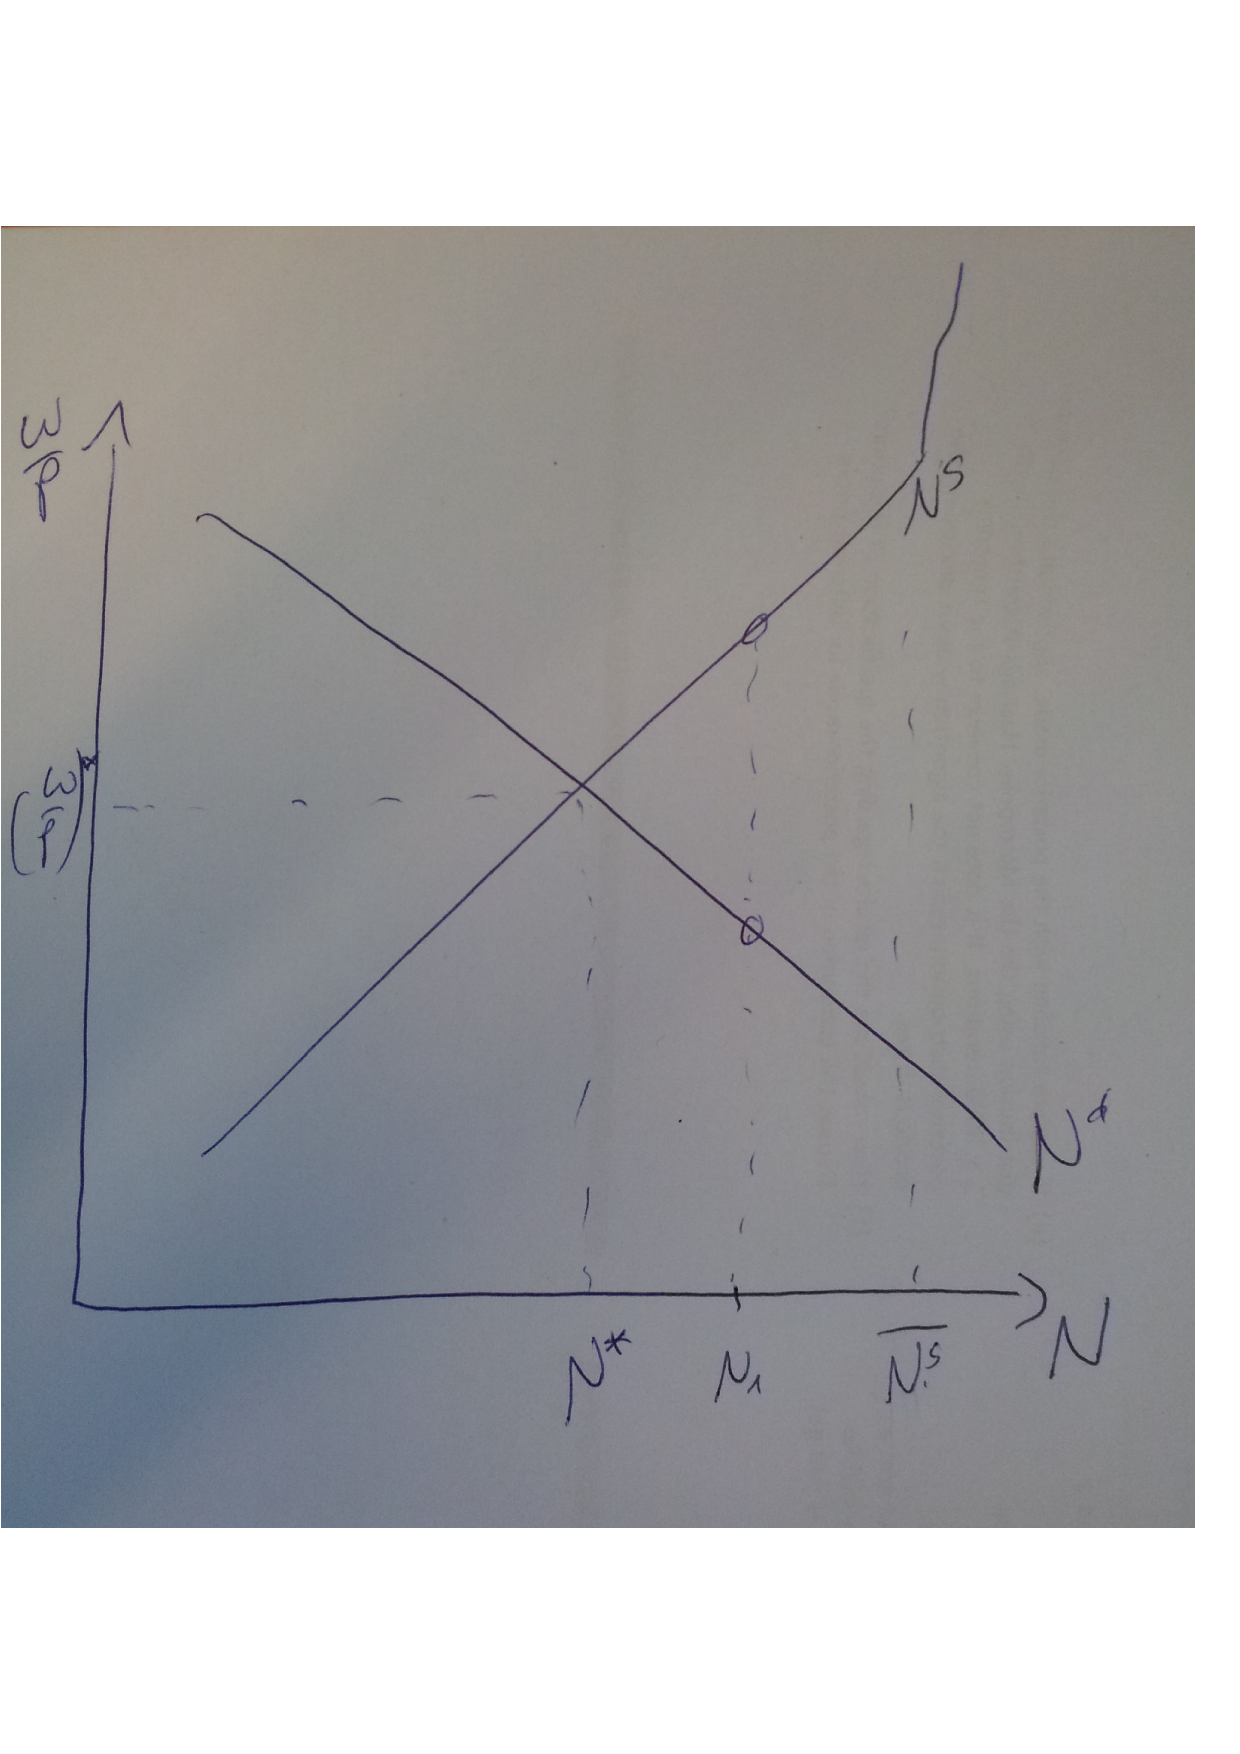
\includegraphics[width=.5\textwidth]{Bilder/Klassik_Arbeitsmarkt.pdf}\\
  Vollbesch\"{a}ftigung: Niemand ist unfreiwillig arbeitslos. D.h. z.B. $(N_1-N^*)$ Arbeitnehmer sind freiwillig arbeitslos, da ihnen der gebotene Reallohn zu gering erscheint. Arbeitslosigkeit im klassisch-neoklassischen Modell bezeichnet nur freiwillige Arbeitslosigkeit! Anhaltende unfreiwillige Arbeitslosigkeit kann der klassisch-neoklassischen Theorie zufolge NICHT auftreten, da der Lohnmechanismus Angebot und Nachfrage ausgleicht!
  \item %\Tree [.{Kapitalmarkt (Handel von WP)} [.Wertpapierangebot [.{\bf Unternehmen} $I(R)=\frac{\Delta B^s}{P}$ ] ] [.Wertpapiernachfrage [.{\bf Haushalte} $S(R)=\frac{\Delta B^d}{P}$  ]  ] ]\\
  Unternehmen beachten bei ihrer Planung die Produktionsm\"{o}glichkeiten abh\"{a}ngig von $F(\underbrace{N}_\text{Auf AM bestimmt},\underbrace{K}_\text{Auf KM bestimmt})$. Investitionen = Ver\"{a}nderung des physischen Kapitalbestandes: $I = K-K_0$. Investitionen werden durch Ausgabe von Wertpapieren finanziert, d.h. $p \cdot I(R) = \Delta B^s$ ist Kapitalnachfrage. Die Haushalte bieten dazu ihre Ersparnisse an, d.h. $p \cdot S(R) = \Delta B^d$. Zinssatz passt sich so an, dass $S(R)=I(R)$ gilt. \\
  Wichtig: $I(R)$ kommt aus der Bedingung f\"{u}r gewinnmaximalen Kapitaleinsatz, $GPK = \frac{\partial F(N,K)}\partial K = R$. Also in jedem Punkt der I-Kurve gilt $GPK = R$, da die I-Kurve alle gewinnmaximalen Kombinationen von Zins und Investitionen abbildet.
  \item G\"{u}termarkt

  \begin{align*}
  Y^S(N) = \underbrace{Y^S(W/P)}_\text{G\"{u}terangebot} = \underbrace{C(i)+I(i)}_\text{G\"{u}ternachfrage}
  \end{align*}
  Gesetz von Walras: Grundidee:
  \begin{tabular}{c|c|c}
    Markt & Unternehmen  & Haushalte \\
  \hline  Arbeitsmarkt& $N^d$  & $N^S$  \\
  \hline  Kapitalmarkt& $I$  & $S$  \\
  \hline  G\"{u}termarkt& $Y^s$  & $C$
  \end{tabular}
  Beide Akteure k\"{o}nnen nur zwei Gr\"{o}{\ss}en frei w\"{a}hlen, die dritte ergibt sich automatisch.\\
  Gesetz von Walras: Die Summe aller \"{U}berschussnachfragen muss gleich null sein.\\
  Implikationen:
  \begin{itemize}
	\item Herrscht auf zwei von drei M\"{a}rkten ein Gleichgewicht, dann ist die \"{U}berschussnachfrage auf dem dritten Markt automatisch null, d.h. der dritte Markt ist ebenso im Gleichgewicht. Bei der makro\"{o}konomischen Analyse gen\"{u}gt es also, das Zustandekommen eines Gleichgewichts auf zwei M\"{a}rkten explizit zu analysieren.
	\item   Bei positiver Summe der \"{U}berschussnachfrage auf zwei M\"{a}rkten muss ein \"{U}berschussangebot auf dem dritten Markt in entsprechender H\"{o}her vorliegen.
  \end{itemize}

\item Quantit\"{a}tsgleichung und Quantit\"{a}tstheorie
\textbf{I) Quantit\"{a}tsgleichung:}\\
1. Wert des G\"{u}terkaufs = gezahlter Betrag, aufsummieren \"{u}ber alle Transaktionen ergibt $P H = Z$, wobei P: Durchschnittspreis aller gekauften G\"{u}ter, H: gesamte Handelsvolumen, Z: Summe aller gezahlten Betr\"{a}ge\\
2. $Z=Mv$ wobei M: Bestand an Zahlungsmitteln, $v$: durschnittliche Verwendungsh\"{a}ufigkeit (Umlaufgeschwindigkeit)\\
1+2: $M v = PH$ dies ist die Quantit\"{a}tsgleichung, eine Identit\"{a}tsgleichung! Problem: in H sind auch Vorleistungen enthalten. F\"{u}r Zusammenhang mit realem Volkseinkommen gilt $Y<H$, d.h. $P_y Y= M v_y$ mit $v_y<v$ die Umlaufgeschwindigkeit im EK-Kreislauf und Y reales Volkseinkommen. $v_y$ ist \"{u}ber Gleichung definiert!\\
Allg:\\
\begin{itemize}
\item KEINE KAUSALEN AUSSAGEN K\"{O}NNEN GETROFFEN WERDEN!
\item \"{A}ndert sich eine Variable, muss sich auch eine andere \"{a}ndern, welche ist unklar.
\end{itemize}
II. Quantit\"{a}tstheorie:\\
Aussagen \"{u}ber den Zusammenhang zwischen Geldmenge und Preisniveau werden abgeleitet: $P=f(M)$
\begin{itemize}
\item Ausgestaltung von f folgt aus der Quantit\"{a}tsgleichung: $P = \underbrace{\frac{v}{Y}}_\text{konstant bzw. exogen} M$
\item Es werden Verhaltensannahmen getroffen:
\begin{itemize}
\item Zahlungsmittel werden gleich oft verwendet, v ist weitgehend konstant und nur von langsam \"{a}ndernden Zahlungsgewohnheiten (exogen) beeinflussbar
\item Realeinkommen ist realwirtschaftliche bestimmt
\end{itemize}
\end{itemize}
Dann l\"{a}sst sich schlie{\ss}en:\\
\enquote{Ver\"{a}nderungen des Preisniveaus werden (in proportionaler Weise) von Ver\"{a}nderungen der Geldmenge bestimmt} --> Kausalit\"{a}t!
Cambridge-Effekt: H\"{o}here Geldmenge f\"{u}hrt zu h\"{o}herer G\"{u}ternachfrage $(Y^d>Y^s)$, aber $Y^s$ konstant. D.h. Preis muss steigen $(P\uparrow)$, aber dann sinkt auch die Nachfrage wieder bis $Y^d=Y^s$ gilt. Reale Geldmenge $\frac{M}{P}$ bleibt konstant!

\item G\"{u}terangebotsfunktion: Wie \"{a}ndert sich die G\"{u}terproduktion, wenn sich das Preisniveau \"{a}ndert. Da die G\"{u}terproduktion vom Arbeitsmarkt abh\"{a}ngt, fragen wir: wie \"{a}ndert sich die Besch\"{a}ftigung, wenn sich der Preis \"{a}ndert. Bei flexiblen Nominall\"{o}hnen, wird jede Preis\"{a}nderung von einer Nominallohn\"{a}nderung begleitet derart, dass der Reallohn unver\"{a}ndert bleibt. Somit bleibt bei flexiblen Nominall\"{o}hnen die Produktion unver\"{a}ndert, die G\"{u}terangebotsfunktion ist konstant und unabh\"{a}ngig von P!\\
    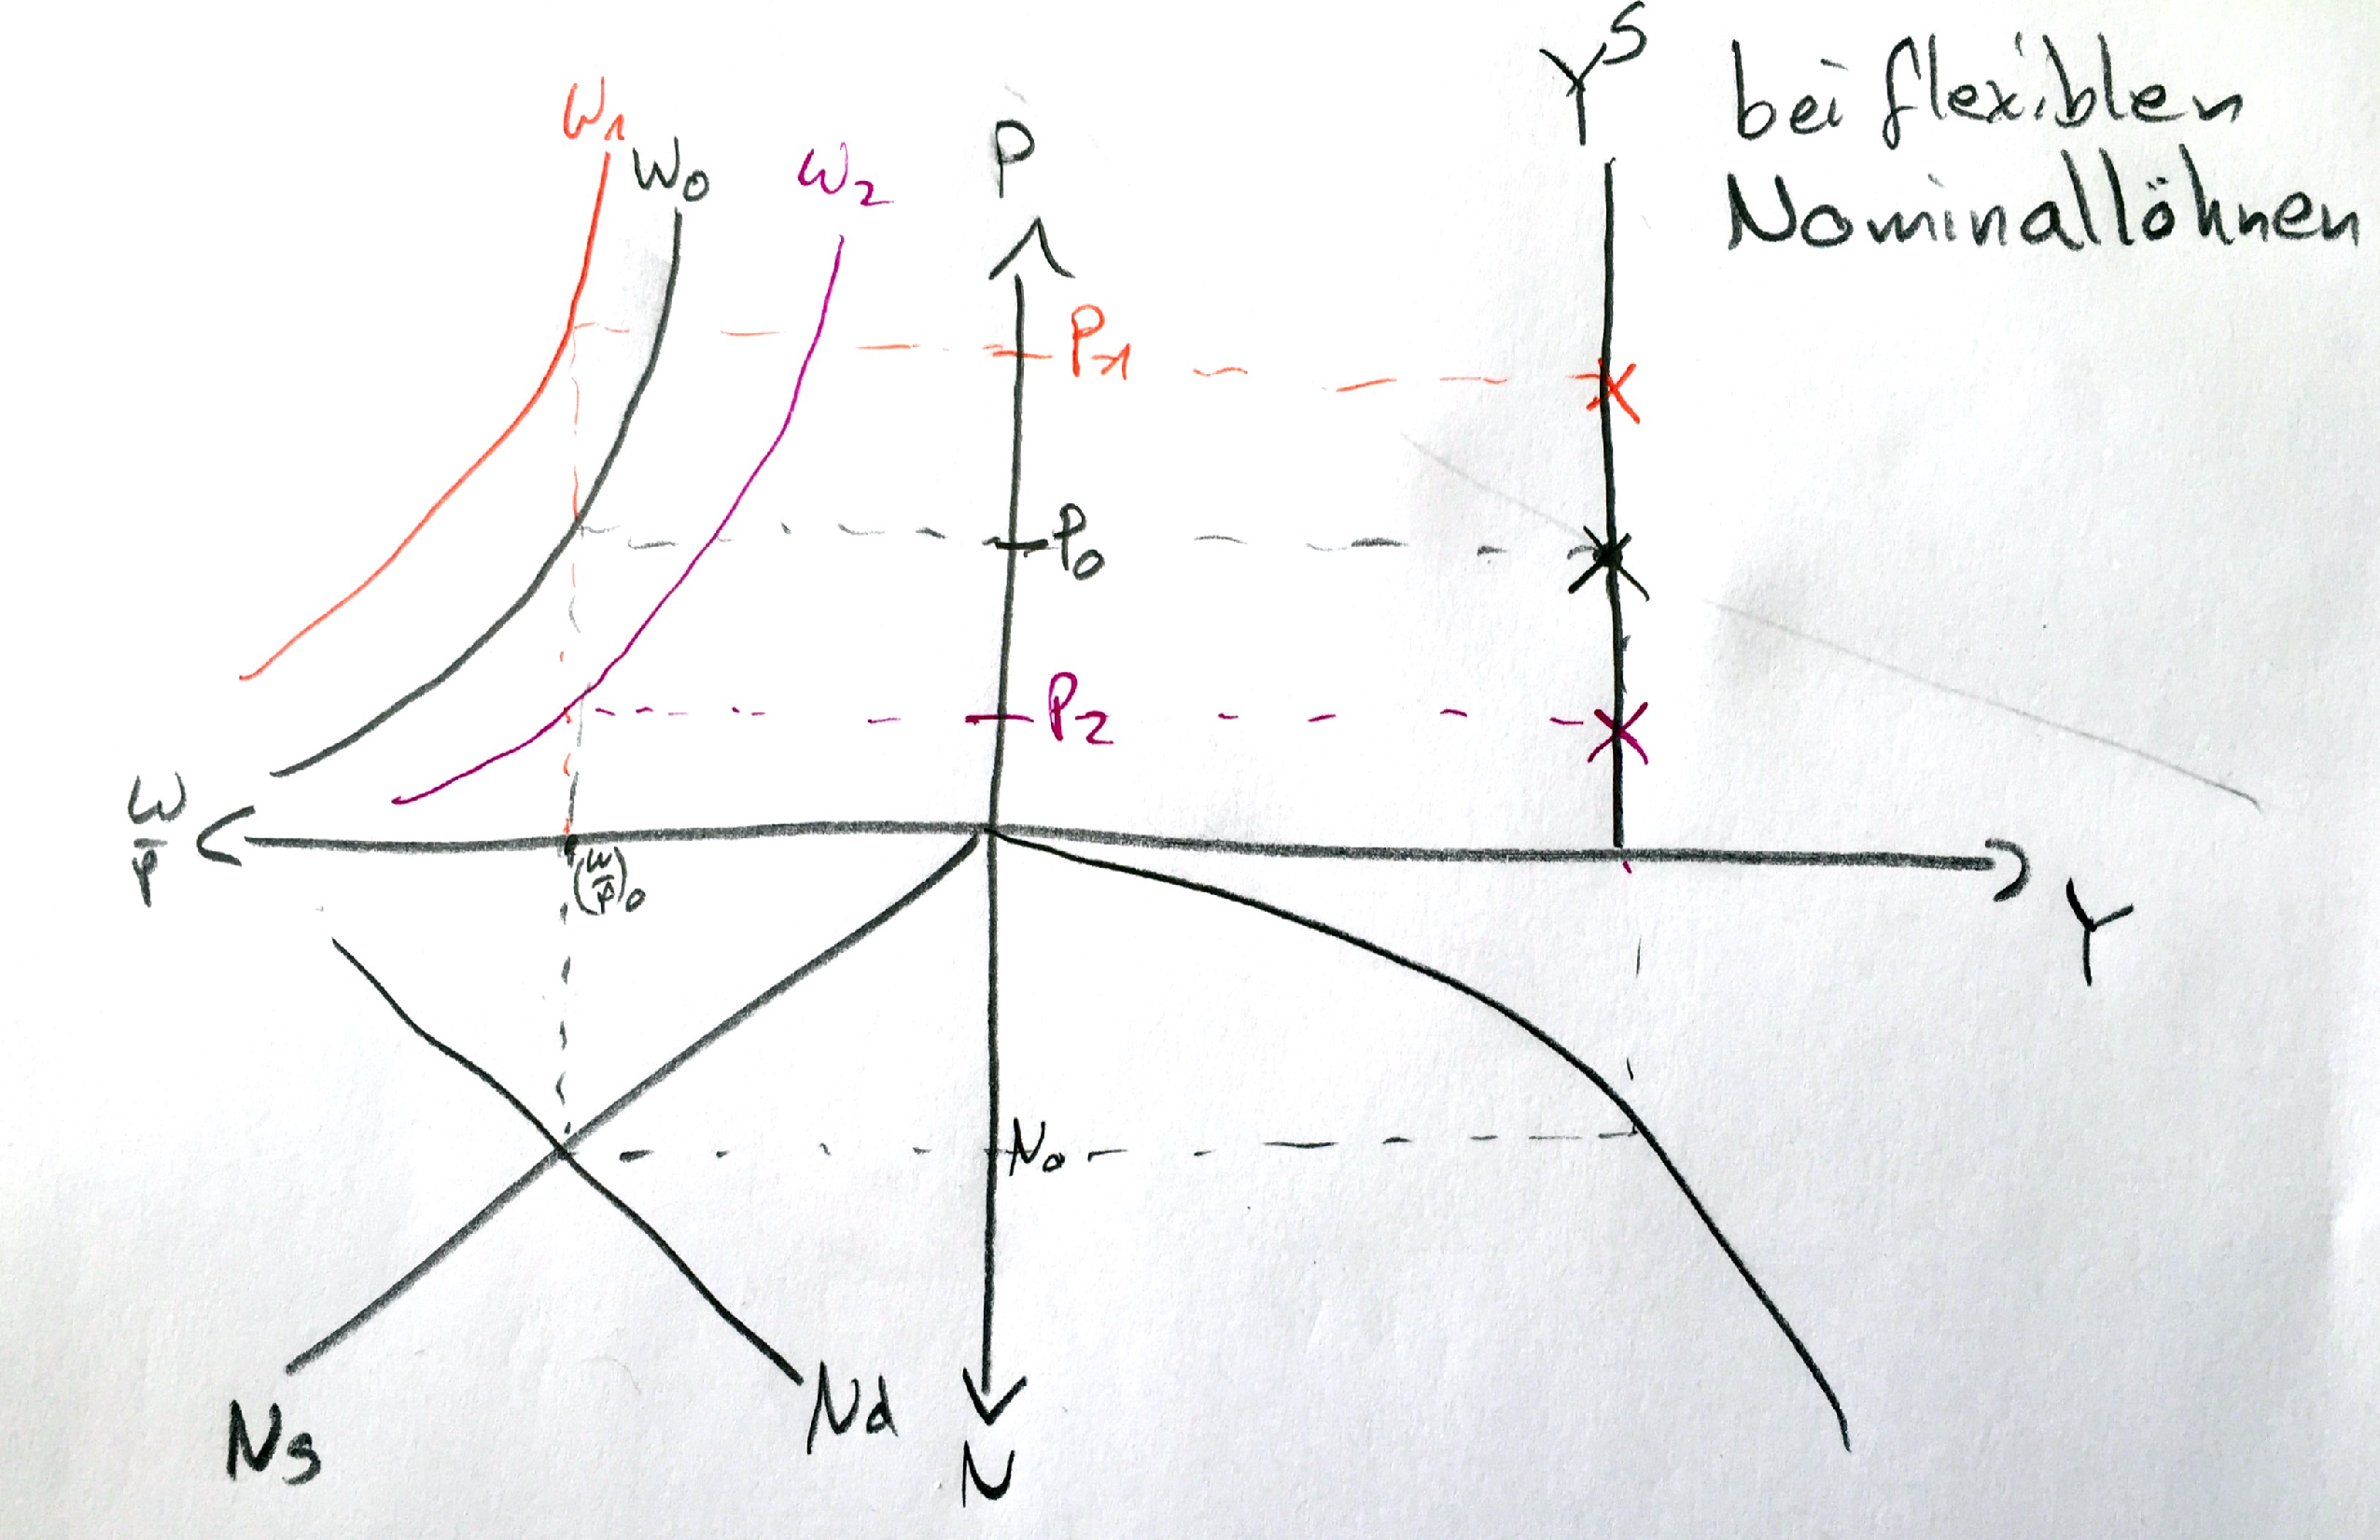
\includegraphics[width=\textwidth]{Bilder/Klassik_AS_Flex.pdf}\\
    Bei fixem Nominallohn verl\"{a}uft die G\"{u}terangebotsfunktion zun\"{a}chst steigend und biegt sich dann zur\"{u}ck, da bei $P>P^*$ der Reallohn sinkt und somit das Arbeitsangebot die k\"{u}rzere Seite ist, w\"{a}hrenddessen bei $P<P^*$ der Reallohn steigt und die Arbeitsnachfrage die k\"{u}rzere Seite ist. In beiden F\"{a}llen f\"{u}hrt dies zu einer geringeren Besch\"{a}ftigung und Produktion.\\
    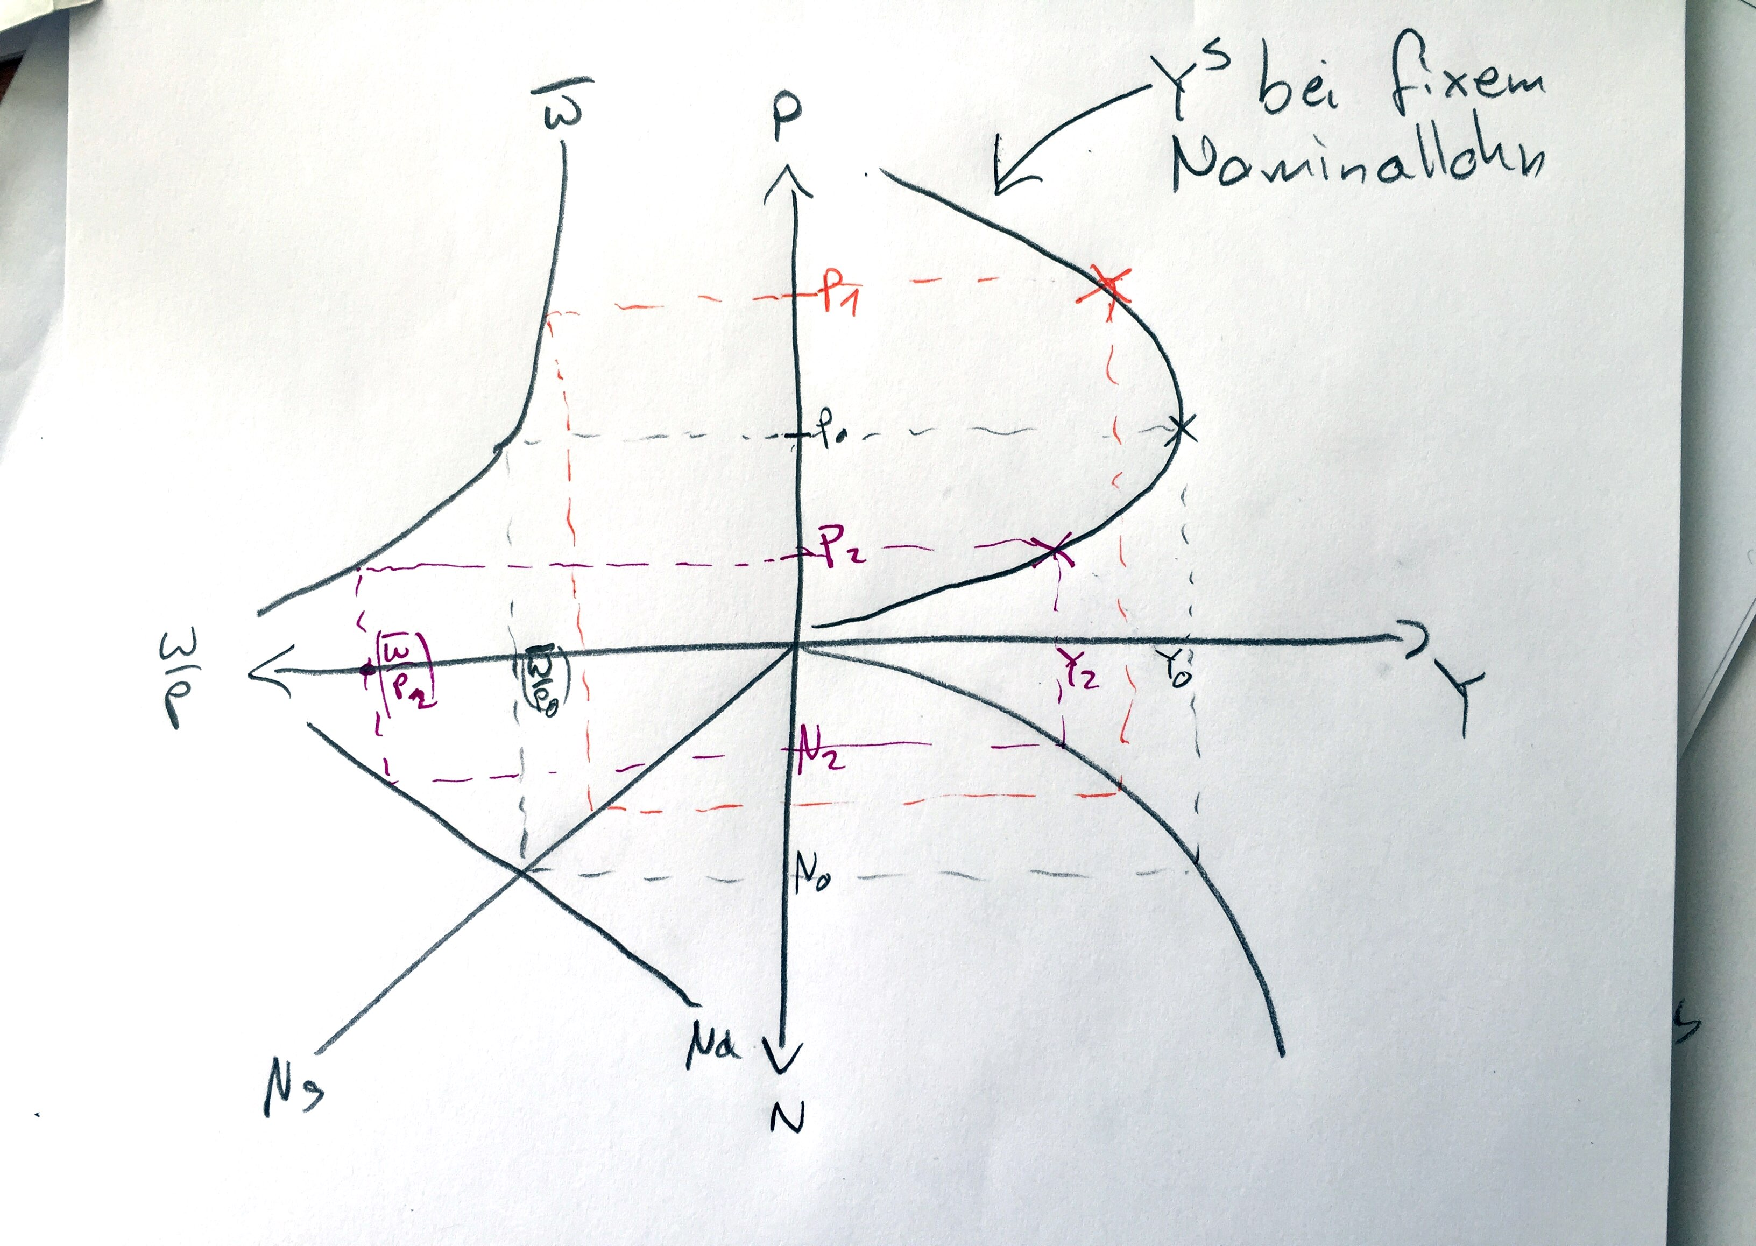
\includegraphics[width=\textwidth]{Bilder/Klassik_AS_Fix.pdf}\\

    Merke: Ys ist eine Konstruktion, sie sagt nichts \"{u}ber das Gleichgewicht aus! Man nehme P0,P1,P2 und tr\"{a}gt die zugeh\"{o}rigen Ys ab. Dann verbindet man die Punkte. Eine Aussage \"{u}ber das Gleichgewicht ist erst mit der Cambridge Gleichung, die hier unser Yd Kurve ist, m\"{o}glich.
\item (Neo-)klassische Gesamtmodell
\begin{align*}
\text{Realer Sektor} = \begin{cases}
\text{(1) Gleichgewicht auf dem Arbeitsmarkt: } N^d(W/P) = N^s(W/P) &\Rightarrow N^*;(W/P)^*\\
\text{(2) Produktionsfunktion: } Y=f(N) & \Rightarrow Y^*\\
\text{(3) Kapitalmarkt: } S(i)=I(i) & \Rightarrow i^*\\
\end{cases}
\end{align*}

\begin{align*}
\text{Monet\"{a}rer Sektor} = \begin{cases}
\text{(4) Quantit\"{a}tstheorie: } P=\frac{Mv}{Y} &\Rightarrow P^*\\
\text{(5) Identi\"{a}t: } W=\frac{W}{P}P & \Rightarrow W^*
\end{cases}
\end{align*}
Realer Sektor determiniert alle realen Gr\"{o}{\ss}en, w\"{a}hrend monet\"{a}rer Sektor nur nominale Gr\"{o}{\ss}en determiniert --> \textbf{DICHOTOMIE}\\
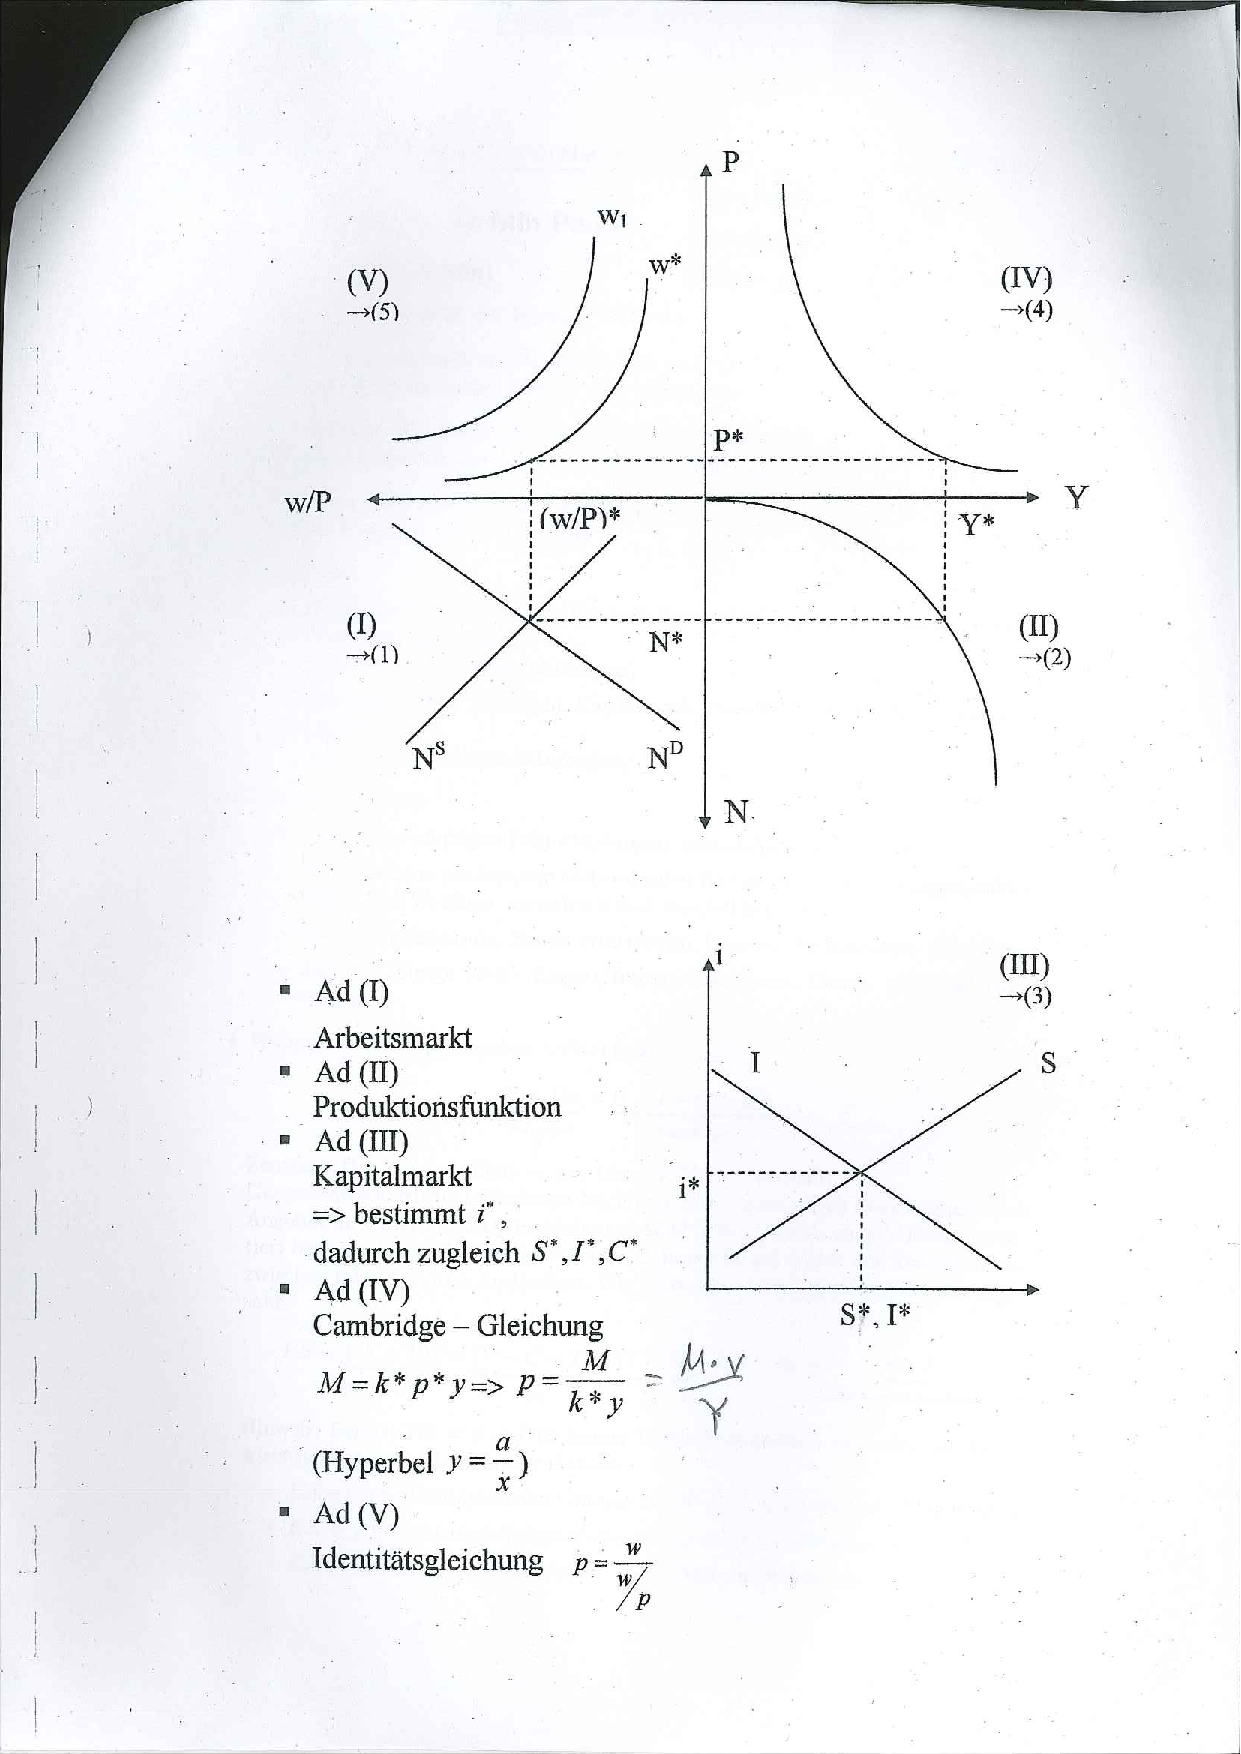
\includegraphics[width=0.75\textwidth]{Bilder/Klassik_Gesamt.pdf}\\
\textbf{Wann verschieben sich die Kurven?}
\begin{itemize}
  \item Produktionsfunktion: Kapitalverbesserung, Technologieniveauverbesserung oder mehr Freihandel: schiebt sich nach au{\ss}en
  \item Arbeitsnachfrage: Analog zur Produktionsfunktion
  \item G\"{u}terangebotsfunktion: Analog zur Produktionsfunktion, allerdings nach rechts unten bzw. links oben.
  \item Arbeitsangebot: Exogene Einflussfaktoren auf Arbeitsangebot
  \item Cambridge-Gleichung: Bei Steigerung von Umlaufgeschwindigkeit oder Geldmenge schiebt sich Kurve nach au{\ss}en
  \item Lohnkurve: Flexibel: Schiebt sich nach au{\ss}en bei Nominallohnsteigerungen oder Preissteigerungen, Fix: schiebt sich einmalig nach au{\ss}en bei Nominallohnsteigerungen
  \item I und S \"{a}ndern sich bei Pr\"{a}ferenz\"{a}nderungen
\end{itemize}
\item Wirtschaftspolitik in der Neoklassik:\\
Modell erweitern:
\begin{align*}
Y &= C+I+G &\text{ G\"{u}termarkt}\\
Y - T &= C+S &\text{ Budgetrestriktion}\\
S &= I + BD	&\text{Kapitalmarkt}\\
BD &= G-T &\text{Staatsbudget, BD ist Budgetdefizit bzw. Neuverschuldung}
\end{align*}
\begin{enumerate}[(i)]
\item Kreditfinanzierte Staatsausgabenerh\"{o}hung: T=0, BD=G, Staat wird auf Kreditmarkt aktiv, d.h.
\begin{align*}
S(i)&=I(i)+BD =I(i)+G\\
Y &= C+S
\end{align*}
Y wird aber \"{u}ber $Y^d=Y^s$ festgelegt.\\
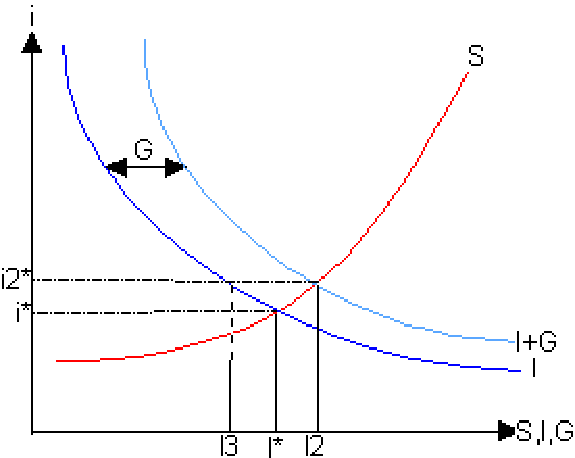
\includegraphics[width=0.5\textwidth]{Bilder/Klassik_Crowding_Out.pdf}\\
2 Effekte:\\
1. $i\uparrow \rightarrow I \downarrow$ Investitions-Crowding-Out\\
2. $i\uparrow \rightarrow S \uparrow \rightarrow C \downarrow$ Konsum-Crowding-Out\\
In Summe ergibt das vollst\"{a}ndiges Crowding-Out, denn Nachfrage muss insgesamt immer noch gleich Angebot sein $Y^d=Y^s$. $Y^s$ wird aber \"{u}ber den Arbeitsmarkt mithilfe der Produktionsfunktion bestimmt! Bei zinsunabh\"{a}ngiger Ersparnis f\"{a}llt das Konsum-Crowding-Out weg: "produktive" Investitionsausgaben werden durch "konsumtive" Staatsausgaben substituiert

\item Steuerfinanzierte Staatsausgabenerh\"{o}hung: $G=T,BD=0$
\begin{align*}
Y - T = Y-G = C+ S
\end{align*}
Y wird aber \"{u}ber $Y^d=Y^s$ festgelegt. Jede Einheit zus\"{a}tzlicher Staatsausgaben geht vollst\"{a}ndig zu Lasten des Konsums und der Ersparnis. Komposition zwischen C und S \"{a}ndert sich, h\"{a}ngt aber von Pr\"{a}ferenzen der Haushalte ab. Wenn S zur\"{u}ckgeht (egal ob zinselastisch oder inelastisch), erh\"{o}ht sich der Zins und die Investitionsnachfrage sinkt. Also auch hier Konsum- sowie Investitions-Crowding-Out.
\item Geldpolitik: Erh\"{o}hung des Geldangebots: $M\uparrow$
\begin{align*}
M = \frac{Y}{v} P\\
M \uparrow \rightarrow P \uparrow
\end{align*}
Cambridge-Effekt!
\end{enumerate}

Merke:\\
(1) Fiskalpolitik nicht erforderlich, da das (neo-)klassische Modell von sich aus das Vollbesch\"{a}ftigungsgleichgewicht erreicht! Fiskalpolitik f\"{u}hrt zu vollst\"{a}ndigem Crowding-Out, da das Arbeitsangebot allein vom Reallohn abh\"{a}ngt und somit die Produktion und Einkommen unver\"{a}ndert bleiben. Nur die Verteilung und der Zins \"{a}ndern sich.\\
(2) Geldpolitik beeinflusst nur das Preisniveau!
\end{enumerate}
\subsection{Rechenaufgabe}
\begin{enumerate}
\item $\frac{\partial Y}{\partial N} = 4\frac{1}{2}N^{-2}=\frac{W}{P} \Leftrightarrow N^d = 4 \left(\frac{W}{P}\right)^{-2}$
\item $N^d=N^s \Leftrightarrow \frac{4}{\left(\frac{W}{P}\right)^2} = 4 - \frac{4}{\left(\frac{W}{P}\right)} \Leftrightarrow 3\left(\frac{W}{P}\right)^2 - 4 \left(\frac{W}{P}\right) - 4 = 0$ ABC oder PQ-Formel ergibt: $(W/P)^*=2,N^*=1,Y^*=4,Lohnsumme=N^* W^* = 2, Lohnquote = Lohnsumme/(PY^*) = 1/2, Gewinn = PY^* - W^*N^* = 2$
\end{enumerate}

\subsection{Kassenhaltungskoeffizient im (neo-)klassischen Modell}
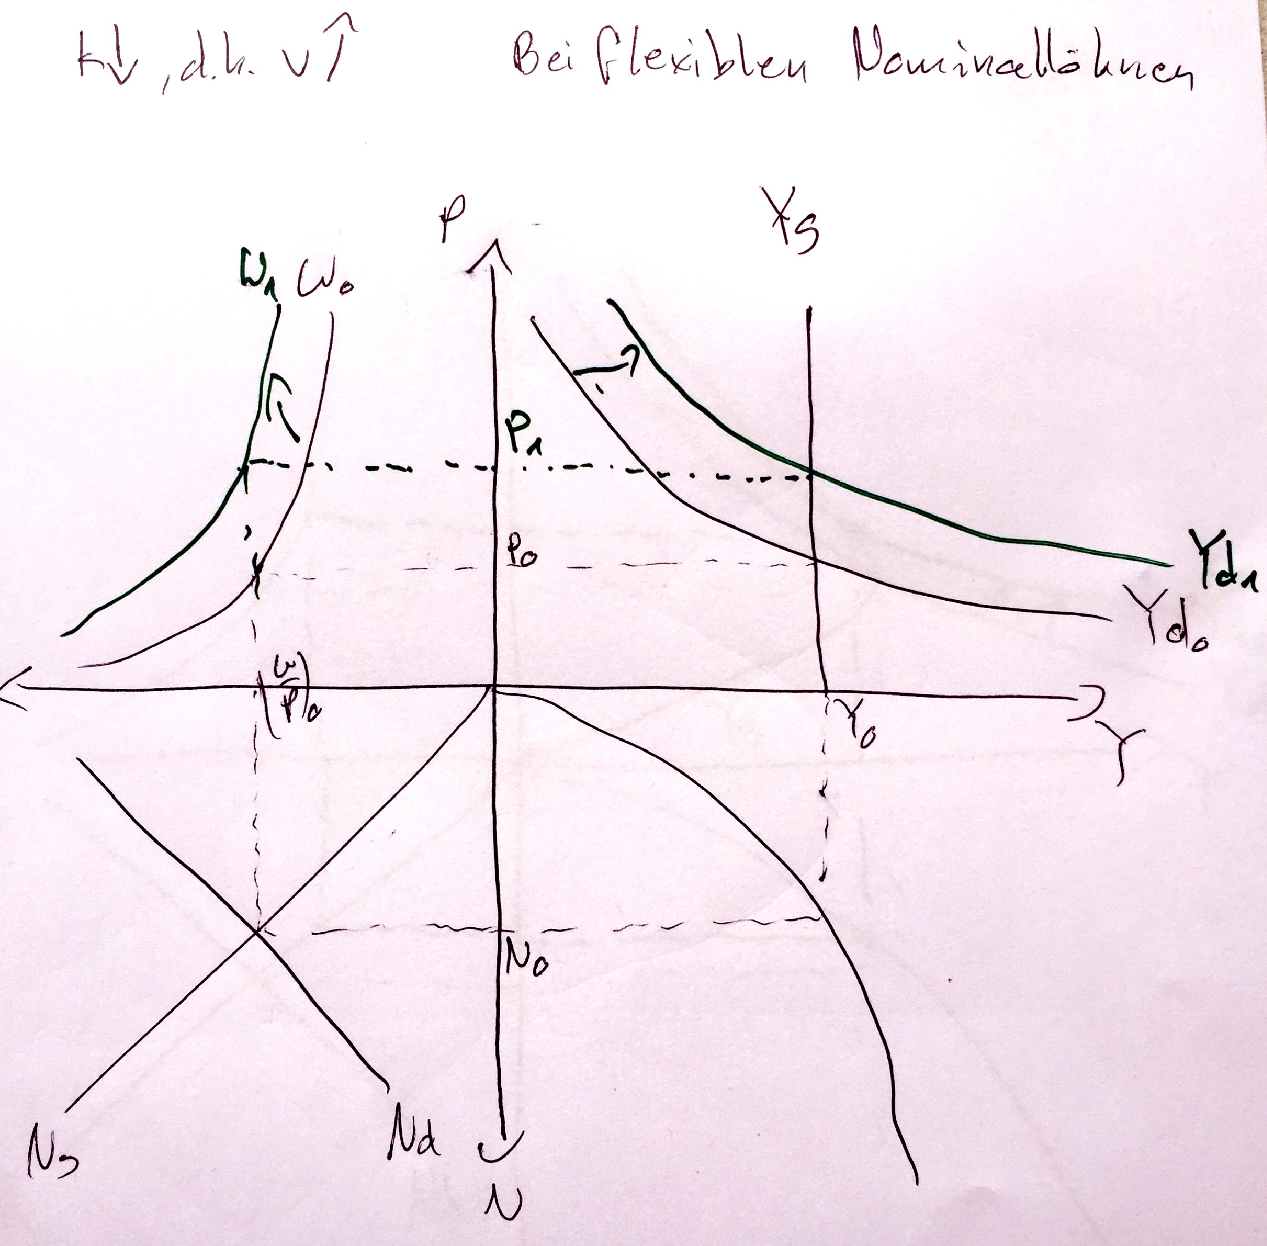
\includegraphics[width=.75\textwidth]{Bilder/Klassik_Kassenhaltung_Flex.pdf}\\
Resultat flexibel: $(W/P)$,$N_s$,$N_d$,$N$,$Y$ unver\"{a}ndert, P und W steigen.\\
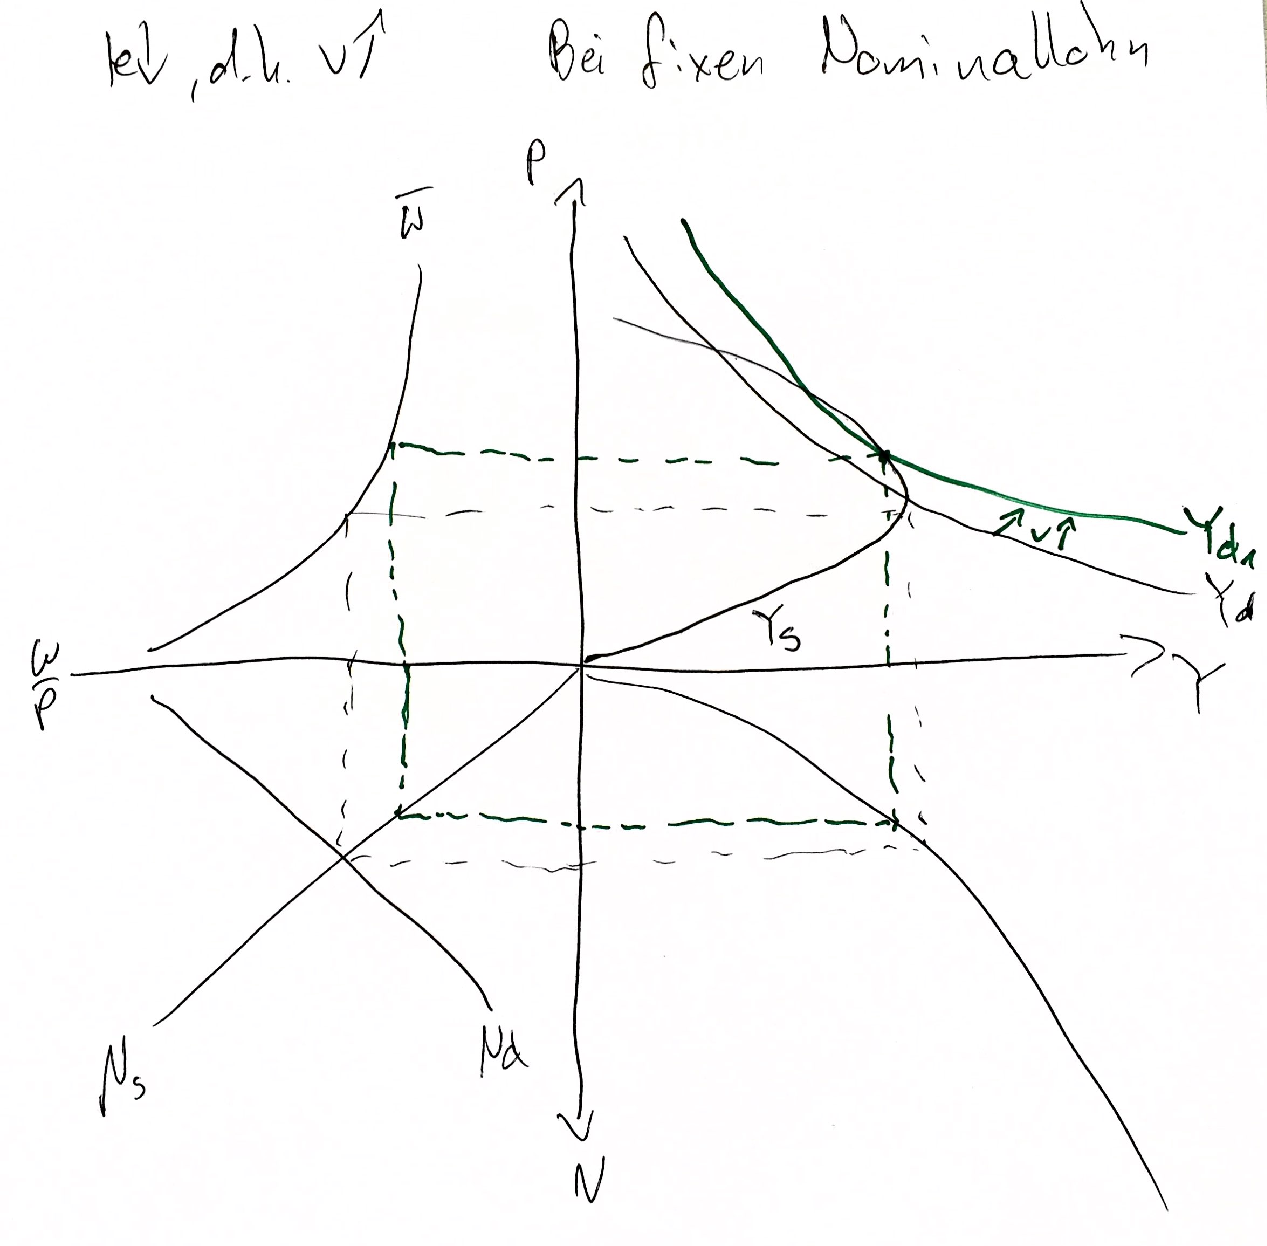
\includegraphics[width=.75\textwidth]{Bilder/Klassik_Kassenhaltung_Fix.pdf}\\
Resultat fix: Preise steigen. Da W fix ist, folgt dass der Reallohn $W/P$ sinkt. Somit sinkt $N_s$, $N_d$ steigt, $N$ sinkt, $Y$ sinkt.

\subsection{Nominallohn im (neo-)klassischen Modell}
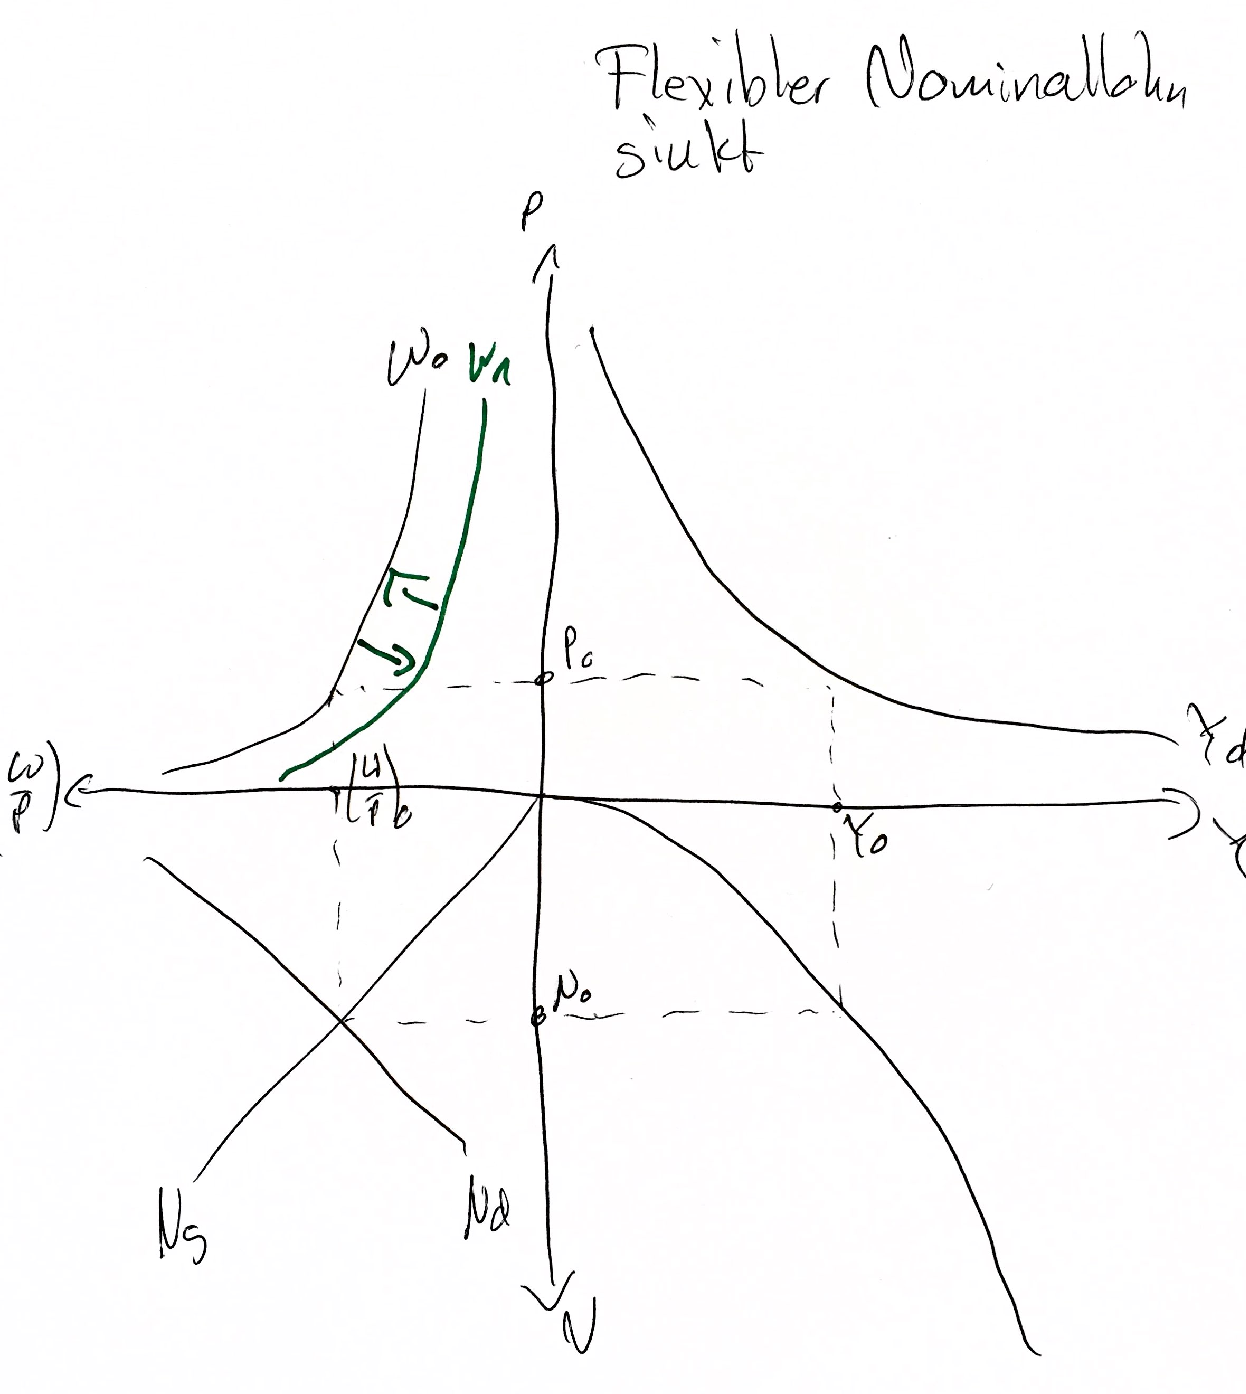
\includegraphics[width=.75\textwidth]{Bilder/Klassik_Nominallohn_Flex.pdf}\\
Resultat flexibel: Alles bleibt unver\"{a}ndert.\\
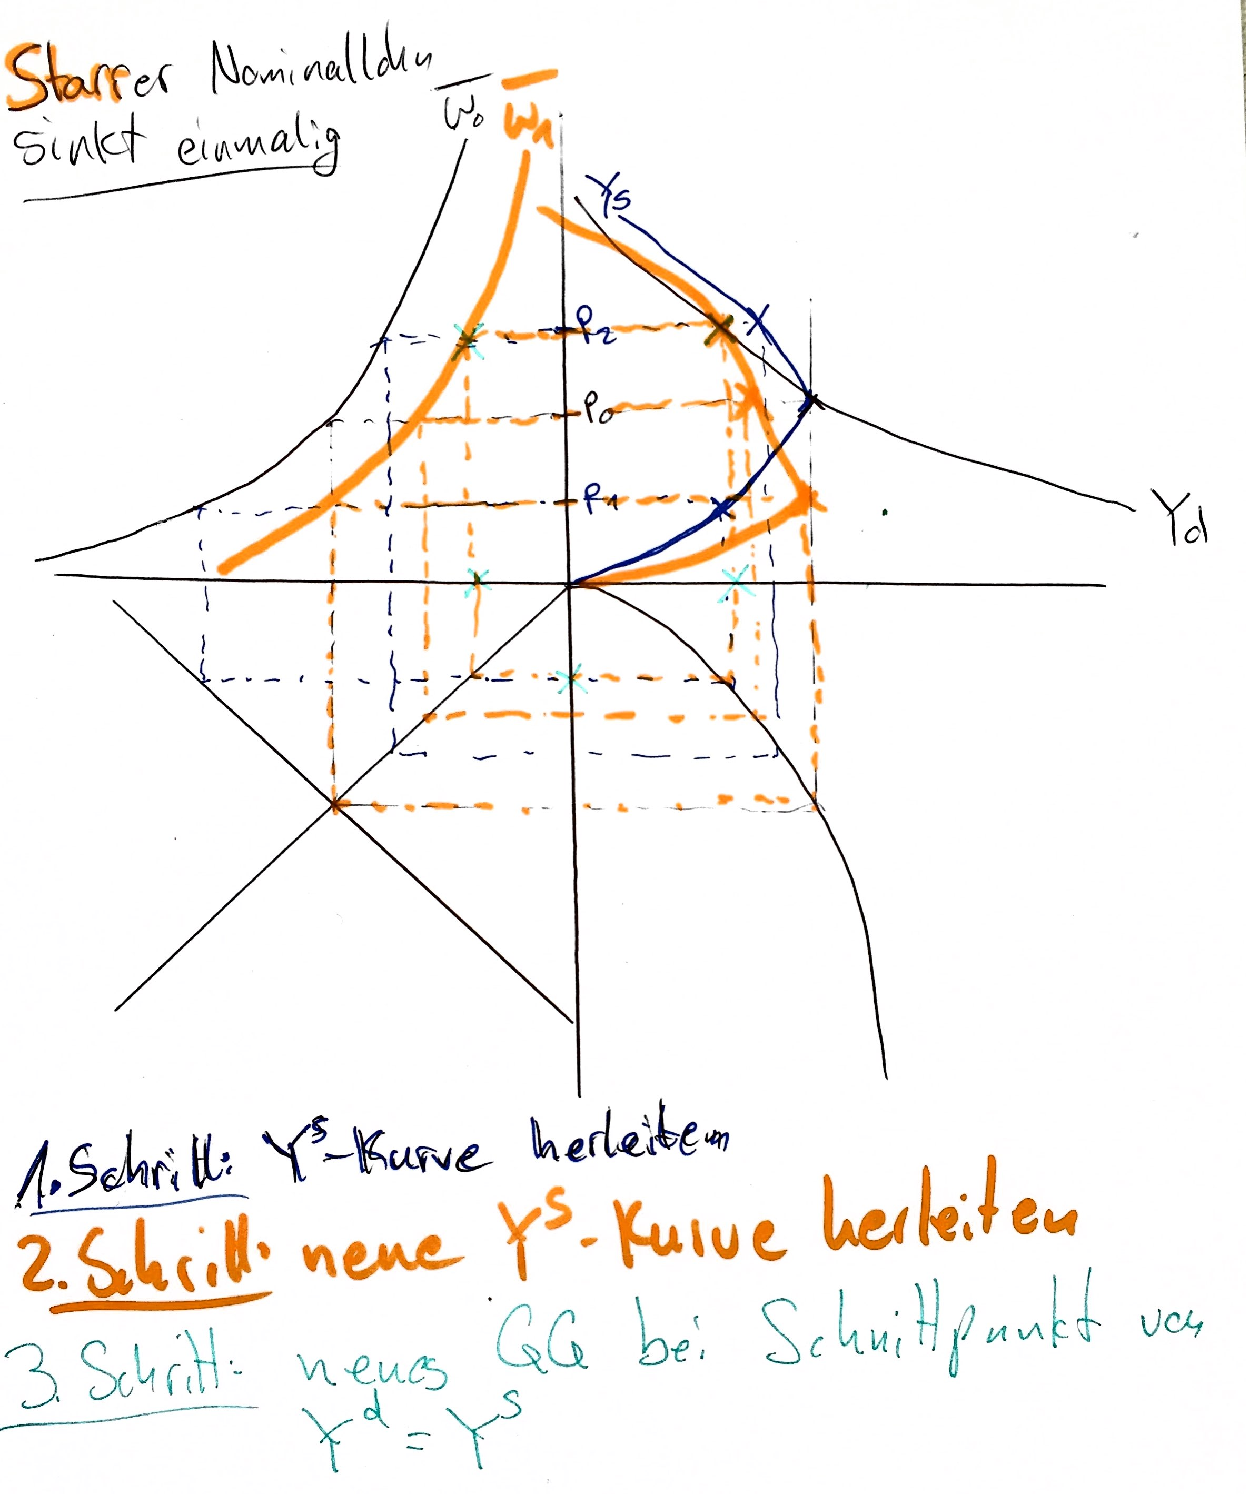
\includegraphics[width=.75\textwidth]{Bilder/Klassik_Nominallohn_Fix.pdf}\\
Bei fixem Nominallohn: W sinkt, dann sinkt auch $W/P$, somit sinkt $N_s$ und $N_d$ steigt. Da $N_s < N_d$ folgt, dass N sinkt. Da N sinkt, sinkt Y und P steigt. Da P steigt, sinkt $W/P$ noch mehr.
Resultat: $W/P$ sinkt, $N_s$ sinkt, $N_d$ steigt, $N$ sinkt, $Y$ sinkt, $P$ steigt, W ist fix auf neuem Wert.
\subsection{Kapitalstock und Geldpolitik im (neo-)klassischen Modell}
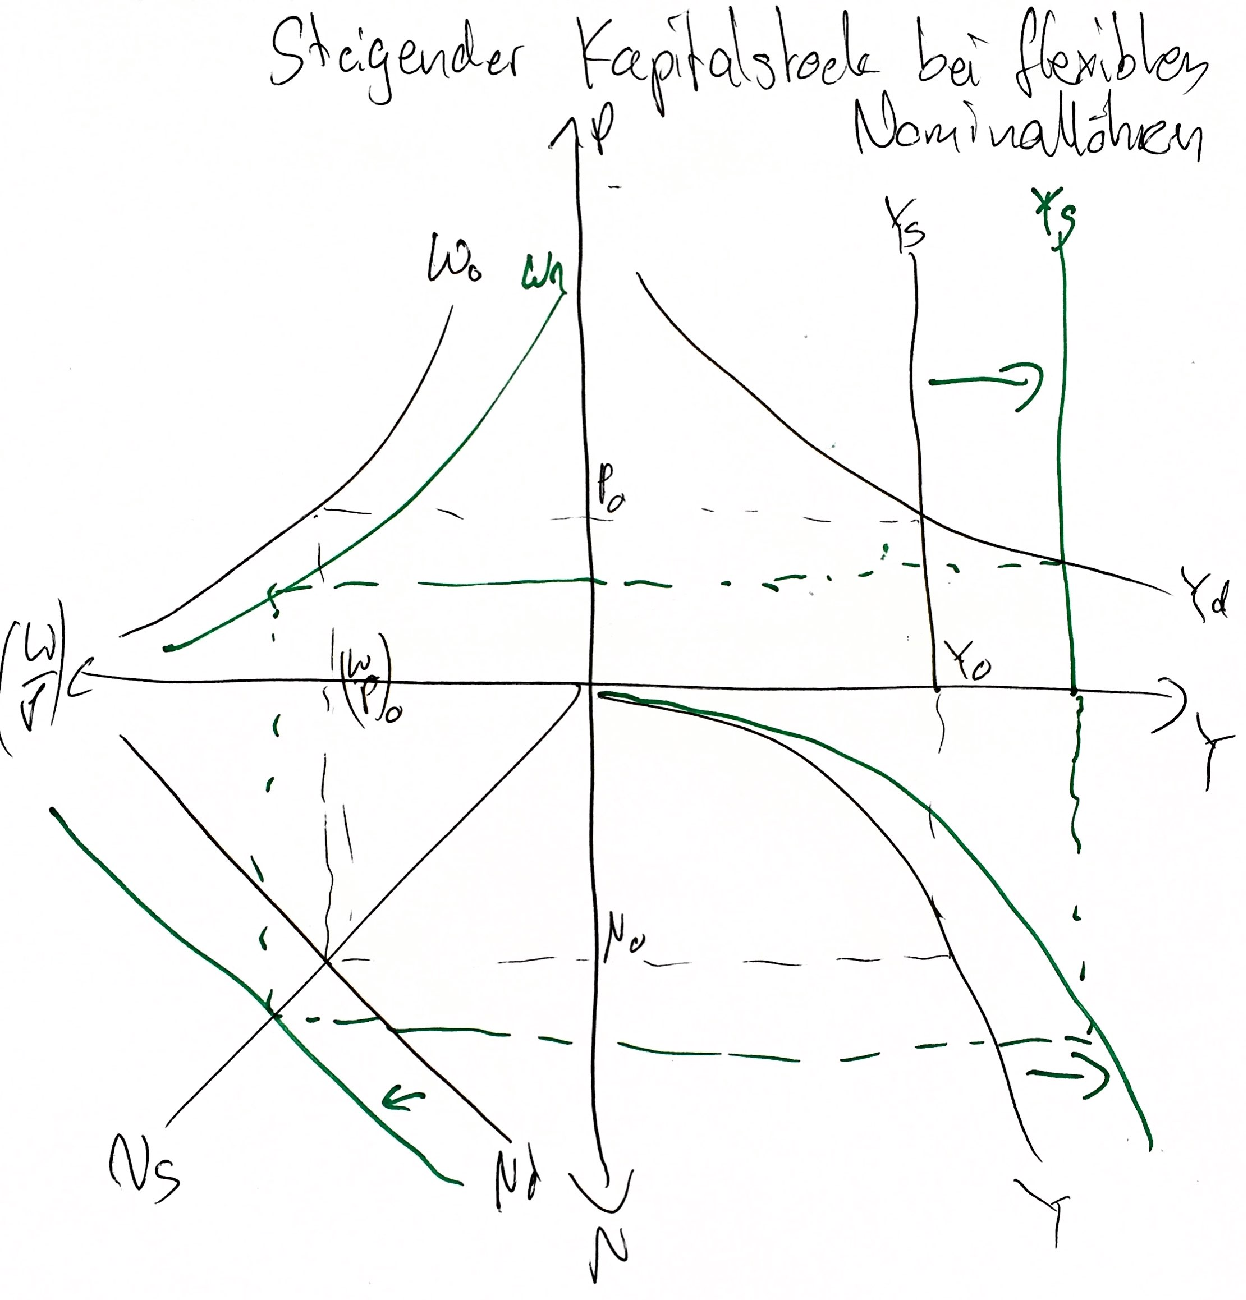
\includegraphics[width=.75\textwidth]{Bilder/Klassik_Kapitalstock_Flex.pdf}\\
Resultat flexibel: $W/P$ steigt, $N_s$ steigt, $N_d$ steigt, $N$ steigt, $Y$ steigt, $P$ sinkt, $W$ sinkt.\\
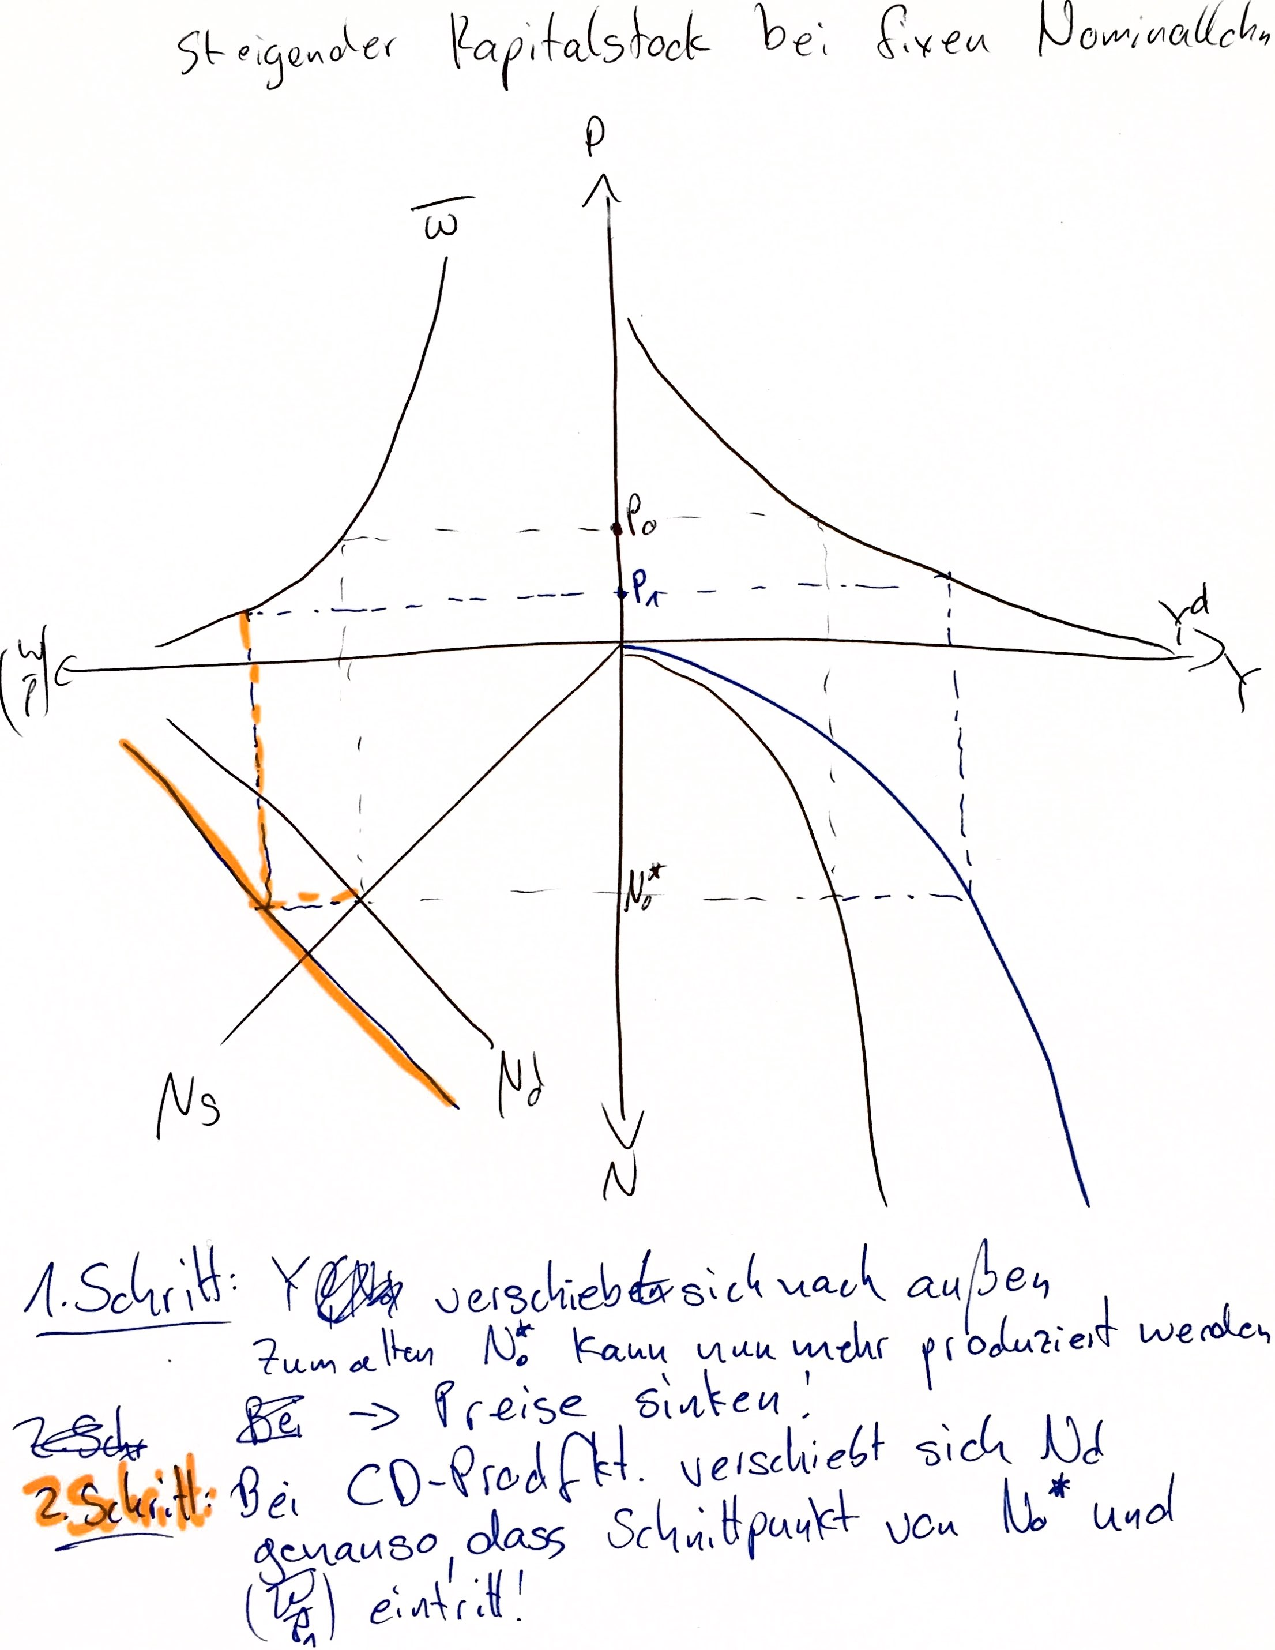
\includegraphics[width=.75\textwidth]{Bilder/Klassik_Kapitalstock_Fix.pdf}\\
Resultat fix: Bei aktuellem $(W/P)^*$ und $N^*$ kann nun mehr produziert werden, d.h. Y steigt. Da Y steigt, sinken die Preise. Da W fix ist, muss der Reallohn $(W/P)$ steigen. Somit steigt $N_s$. Einfluss auf $N_d$ unklar, h\"{a}ngt von Elastizit\"{a}ten ab. Bei Cobb-Douglas Produktionsfunktion bleibt $N_d=N^*$ unver\"{a}ndert.
Also: $W/P$ steigt, $N_s$ steigt, $N_d$ unver\"{a}ndert, $N$ unver\"{a}ndert, $Y$ steigt, $P$ sinkt, $W$ sinkt.
\subsection{Verst\"{a}ndnisfragen}
\begin{enumerate}
\item wahr, BR gilt immer f\"{u}r alle Kombis
\item falsch, da Arbeitsnachfrage steigt f\"{u}r jeden Lohn
\item wahr, im klassischen Modell gilt die Dichotomie
\item wahr
\item wahr, da ABS zinsunelastisch sind.
\item falsch
\item wahr, falls zinsabh\"{a}ngige Ersparnis.
\item falsch, \"{U}berschussangebot
\item wahr
\item falsch, Zinssatz steigt
\item falsch, Walras Gesetz erm\"{o}glicht es, dass z.B. \"{U}A auf Kreditmarkt und \"{U}N auf Arbeitsmarkt
\item falsch
\item falsch
\item wahr
\item falsch, Arbeitslosigkeit ist ein \"{U}A, d.h. auf Kreditmarkt muss \"{U}N sein
\item falsch, nur wenn \"{U}A auf Markt 1 genau gleich \"{U}N auf Markt 2. Im allgemeinen nicht.
\item falsch, Gesetz gilt immer.
\item falsch, Quantit\"{a}tsgleichung trifft hier keine Aussage
\item falsch, Sinken der Geldmenge f\"{u}hrt zu sinkenden Preisen, das Sozialprodukt wird auf dem AN bestimmt
\item wahr
\item falsch
\item falsch, keine Aussage \"{u}ber positiv oder negativ
\item wahr
\item falsch, Preis ist abh\"{a}ngig von der Geldmenge
\item wahr
\item falsch
\item wahr
\item wahr
\item falsch, Kausalit\"{a}t ist andersrum.
\item falsch, keine Aussagen m\"{o}glich wegen Y und v
\item falsch, Preisniveau nur von Geldmenge abh\"{a}ngig
\item falsch, keine Aussagen m\"{o}glich wegen Y und v
\item falsch, Theorie unterstellt Kausalit\"{a}t
\item wahr
\item falsch, Einkommen wird auf anderen M\"{a}rkten bestimmt
\item wahr, $k=1/v$
\item wahr
\item falsch, Preise passen sich an
\item falsch, keine Aussagen m\"{o}glich wegen Y und v
\item wahr
\end{enumerate}




\section{Keynesianische Theorie}
\subsection{Keynesianische Kreuz, Sparfunktion und Multiplikator}
\begin{enumerate}[(a)]
\item Fundamentale Unterschiede zur neoklassischen Theorie:
\begin{itemize}
\item Gleichgewichtsbegriff
\begin{itemize}
  \item Klassik-GG: Marktr\"{a}umung
  \item Keynes-GG: Keine inneren Anreize zum Abweichen
\end{itemize}
\item Lohn- und Preisrigidit\"{a}ten\\
Hindernisse erschweren insbesondere Lohn- und Preissenkungen:
    \begin{itemize}
      \item Vermachtung (Marktkonzentration)
      \item Psychologische Ursachen
      \item Institutionelle Ursachen (Vertragslaufzeiten)
    \end{itemize}
    Preise nehmen nicht zwangsl\"{a}ufig Marktr\"{a}umungswerte an, d.h. umgesetzte Mengen bestimmt durch Minimumsregeln $Y=min(Y^s,Y^d)$, k\"{u}rzere Seite gewinnt.
\item Effektive Nachfrage\\
    Die gesamtwirtschaftliche Nachfrage bestimmt das Niveau von Produktion (Angebot) und Besch\"{a}ftigung. F\"{u}r Konsum ist tats\"{a}chliches verf\"{u}gbares Einkommen relevant. Ungenutzte Produktionsm\"{o}glichkeiten erzeugen
wegen mangelndem Absatz Arbeitslosigkeit. Unternehmen sind auf G\"{u}termarkt rationiert (effektive G\"{u}ternachfrage). Haushalte sind auf Arbeitsmarkt rationiert (effektive Arbeitsnachfrage).\\Schematisch:\\
    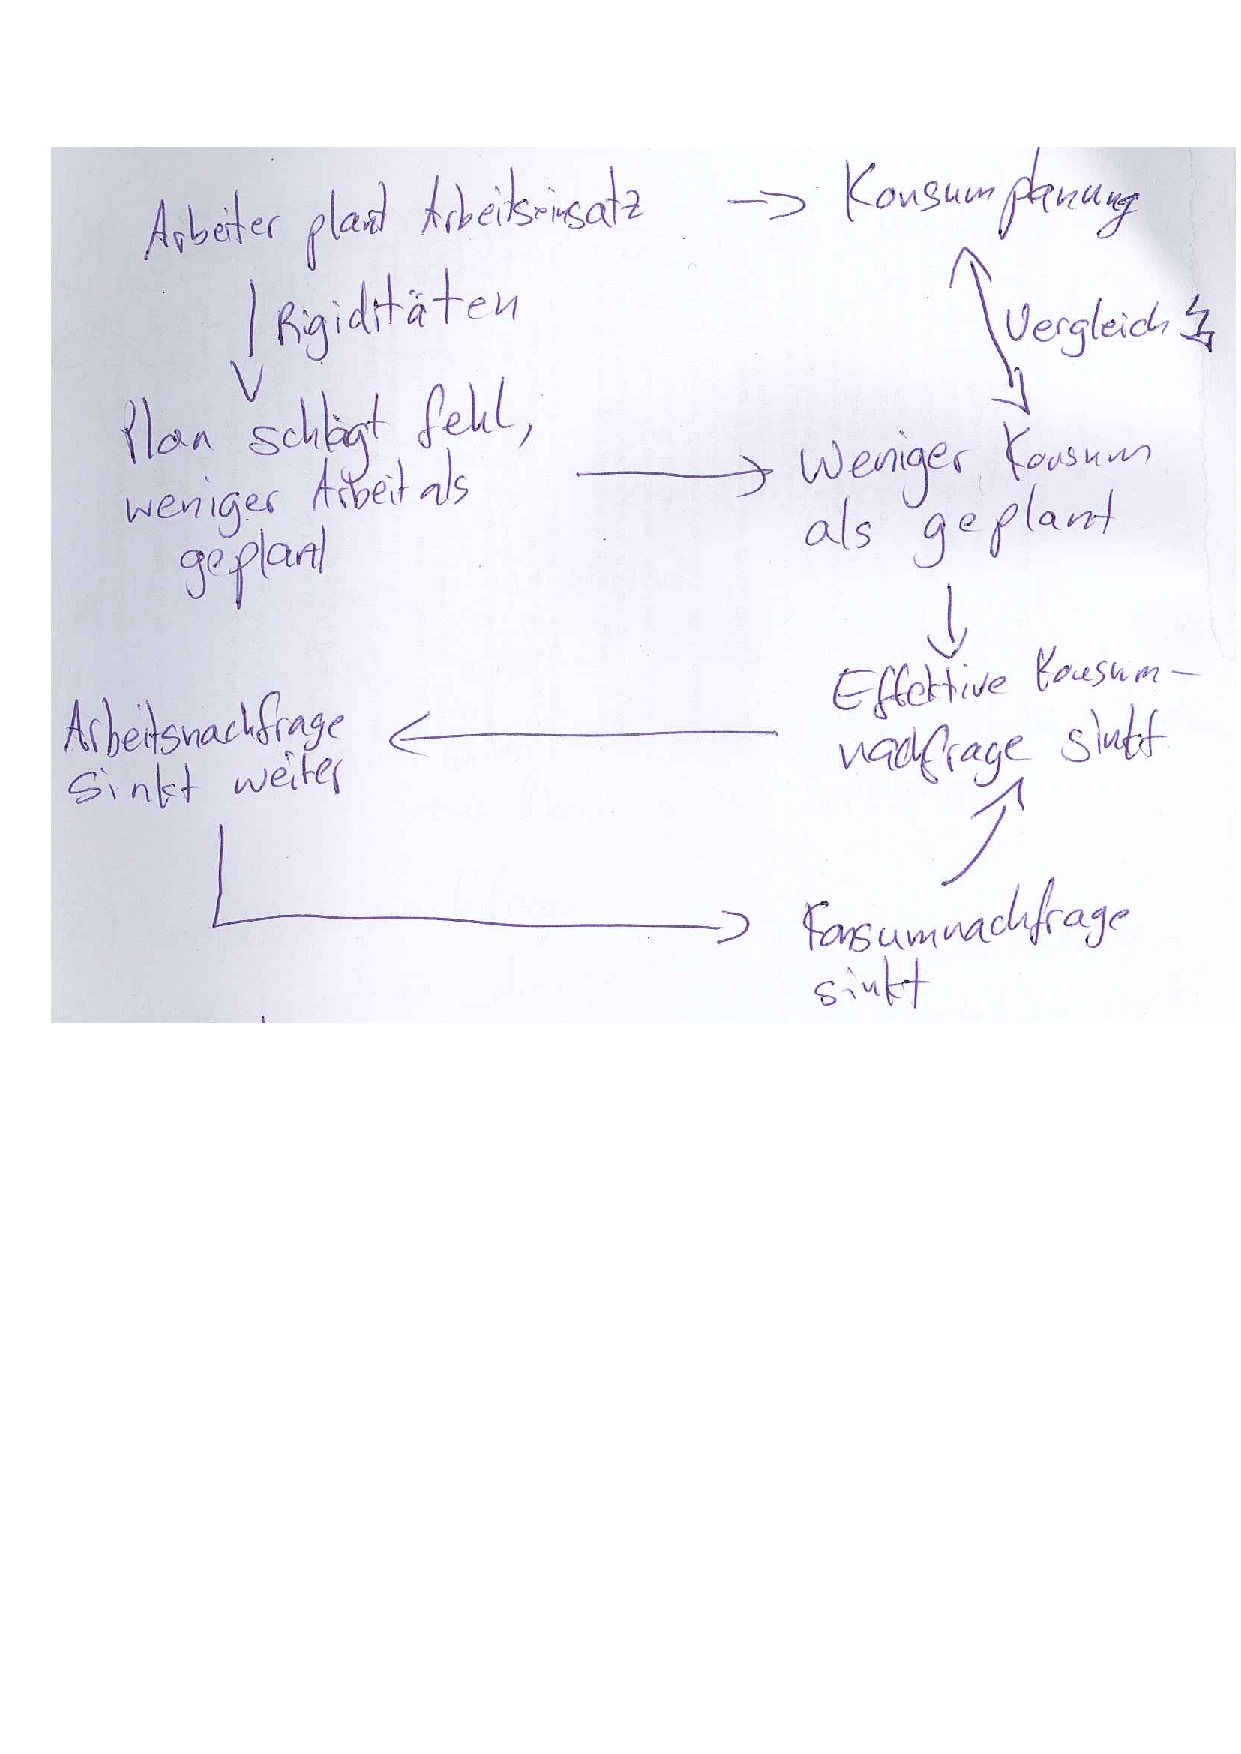
\includegraphics[width=\textwidth]{Bilder/Keynes_Effektive_Nachfrage.pdf}
\end{itemize}
\item Verhaltensgleichungen (basierend auf Keynes Annahmen)
\begin{enumerate}[(1)]
  \item Konsumnachfrage (linear): $\underbrace{C}_{endogen}=\underbrace{C_{aut}}_\text{exogen} + \underbrace{c}_{Parameter} \underbrace{Y}_\text{endogen}$\\
  Konsum heute h\"{a}ngt vom verf\"{u}gbaren Einkommen \emph{heute} ab und nicht von Plangr\"{o}{\ss}en! $C_{aut}$ ist autonomer Konsum und $c = \partial C / \partial Y$ die sogenannte marginale Konsumneigung.\\
  Unterschiede zur Neoklassik:
  \begin{itemize}
    \item Kein intertemporaler Ausgleich (Konsum nicht vom Zins abh\"{a}ngig)
    \item Keine simultane Planung von EK und Konsum bzw. Planung ist irrelevant
  \end{itemize}
  \item Investitionsnachfrage (hier: Zinsabh\"{a}ngig!)\\
  Idee: Investiere solange bis die Grenzleistungsf\"{a}higkeit einer zus\"{a}tzlichen Investition gr\"{o}{\ss}er als der Zins ist. Grenzleistungsf\"{a}higkeit des Kapitals nimmt mit einer zus\"{a}tzlichen Einheit Kapital ab: $I=I(\overset{-}{i})=\underbrace{I_{aut}}_\text{exogen} - b \underbrace{i}_\text{hier exogen,da i gegeben sp\"{a}ter endogen}$.\\
  Funktional \"{a}hnlich der neoklassischen Investitionsfunktion, aber Einsch\"{a}tzung der Grenzleistungsf\"{a}higkeit ist stark psychologisch bestimmt (interner Zinssatz einer Investition)\\
  HIER NOCH ETWAS BESSER!!!!
  \item Aggregierte Nachfrage (Identit\"{a}tsgleichung), effektive Nachfrage, $Y^d = C+I$, alles endogen
  \item Im Gleichgewicht gilt Nachfrage = Angebot $(Y^s=Y^d)$, insbesondere bei Keynes antizipierte Nachfrage = tats\"{a}chliche Nachfrage
  \item Unternehmen passen Produktion an erwartete Nachfrage an:
  \begin{itemize}
    \item Einkommen der Haushalte in H\"{o}he des Outputs
    \item Einkommen wird durch Produktion bestimmt
    \item Einkommen ist f\"{u}r Haushalte fix
  \end{itemize}
  HIER NOCH GENAUER!\\
  $(3)+(4)+(5) \Rightarrow Y^s=Y=Y^d$, Y ist endogen!
\end{enumerate}

\item \textbf{Absolute Einkommenshypothese}: Konsum heute h\"{a}ngt vom Einkommen heute ab, nicht vom Einkommen folgender Perioden. Zus\"{a}tzliches Einkommen wird gem\"{a}{\ss} marginaler Neigungen konsumiert. Stabilit\"{a}t durch Multiplikatorprozess ist m\"{o}glich, Konsum jedoch stark von aktueller Konjunktur abh\"{a}ngig. Dies ist die betrachtete Keynesianische Konsumfunktion.\\
    \textbf{Permanente Einkommenshypothese:} Konsumverhalten orientiert sich am durchschnittlichem Einkommen. Vor\"{u}bergehende Einkommens\"{a}nderungen haben keine \"{A}nderung des Konsumverhaltens zur Folge. Sehr stabilisierend, da Einkommens\"{a}nderungen Konsumnachfrage kaum ver\"{a}ndern.
\item \textbf{Sparfunktion:}
\begin{itemize}
\item \textbf{\emph{Analytische Herleitung:}}
    \begin{align*}
      S=Y-C=Y-C_{aut}-c Y = -C_{aut}+(1-c) Y\\
      \Leftrightarrow S = -C_{aut} + \underbrace{(1-c)}_{\equiv s} Y = -c_{aut} + s Y
    \end{align*}
    Marginale Konsumneigung: $\frac{\partial C}{\partial Y} = c$ und marginale Sparneigung: $\frac{\partial S}{\partial Y} = 1-c\equiv s$
\item \textbf{\emph{Grafische Herleitung}}
\begin{center}
  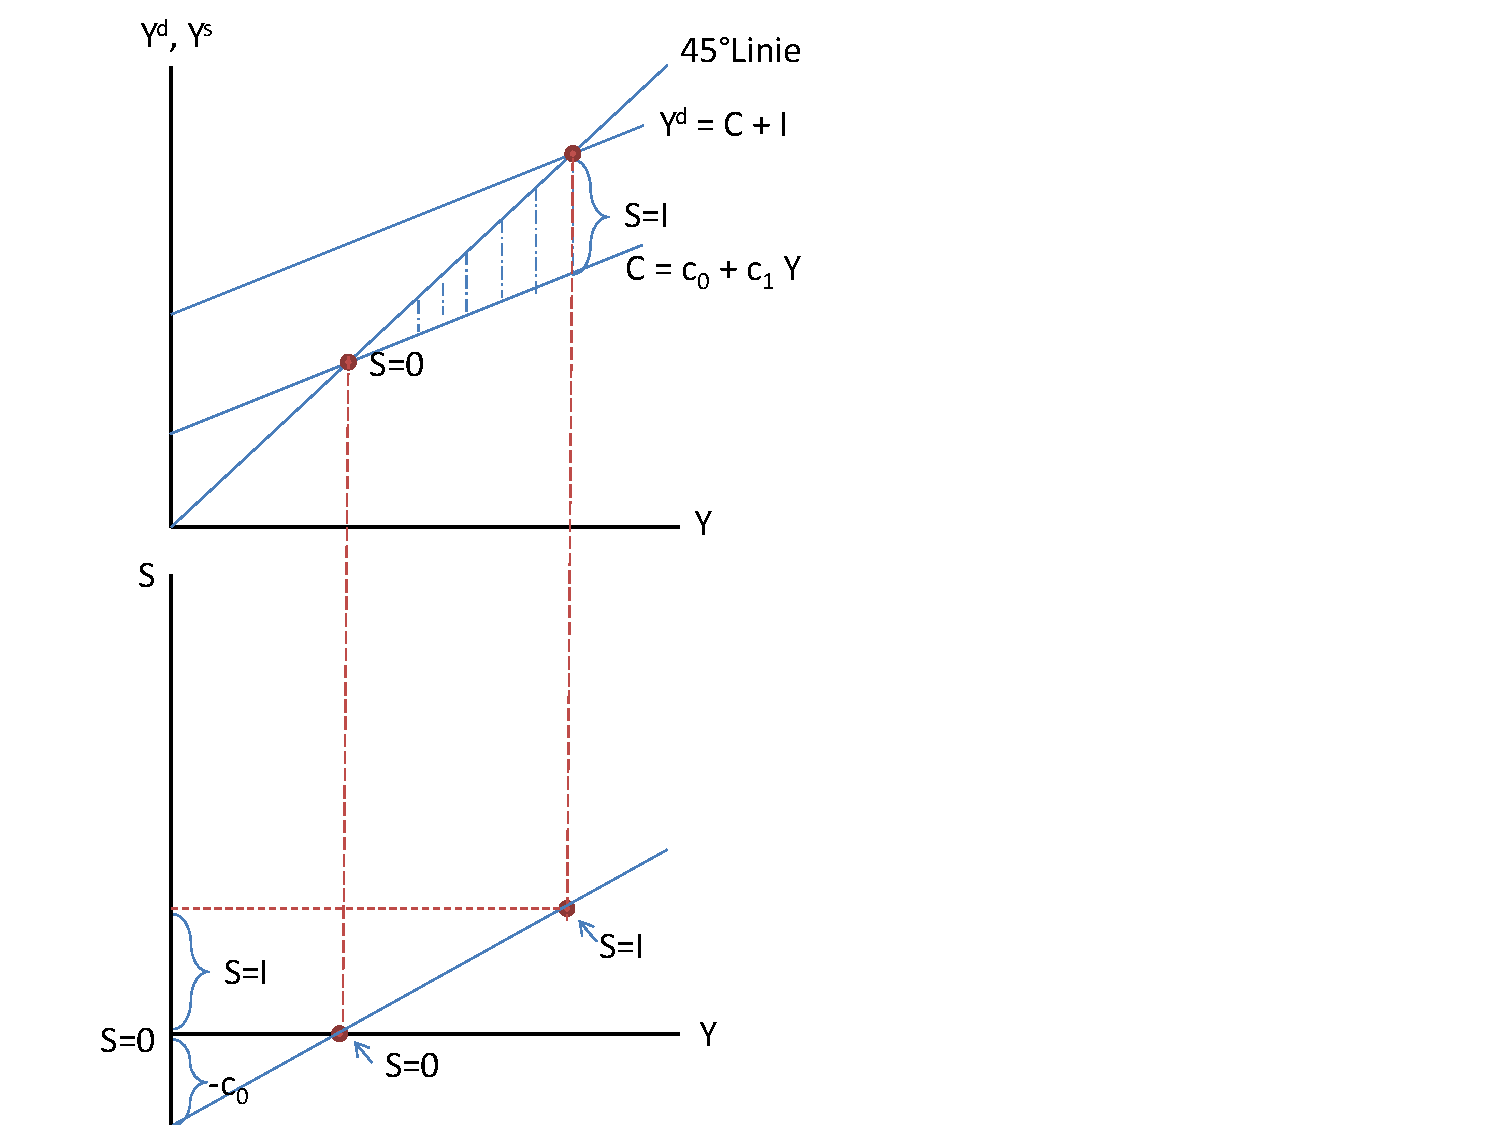
\includegraphics[width=.7\textwidth]{Bilder/Keynes_Sparfunktion.pdf}\\
\end{center}
HIER NOCH UMGEDREHT!
\end{itemize}

\item
\textbf{Bestimmung des gleichgewichtigen Einkommens}
\begin{enumerate}[(i)]
  \item Keynesianische Kreuz
  \begin{align*}
    Y=C+I=C_{aut}+c Y + I_{aut} -b i\\
    Y= \frac{1}{1-c} (C_{aut} + I_{aut} - b i)
  \end{align*}
  \begin{center}
  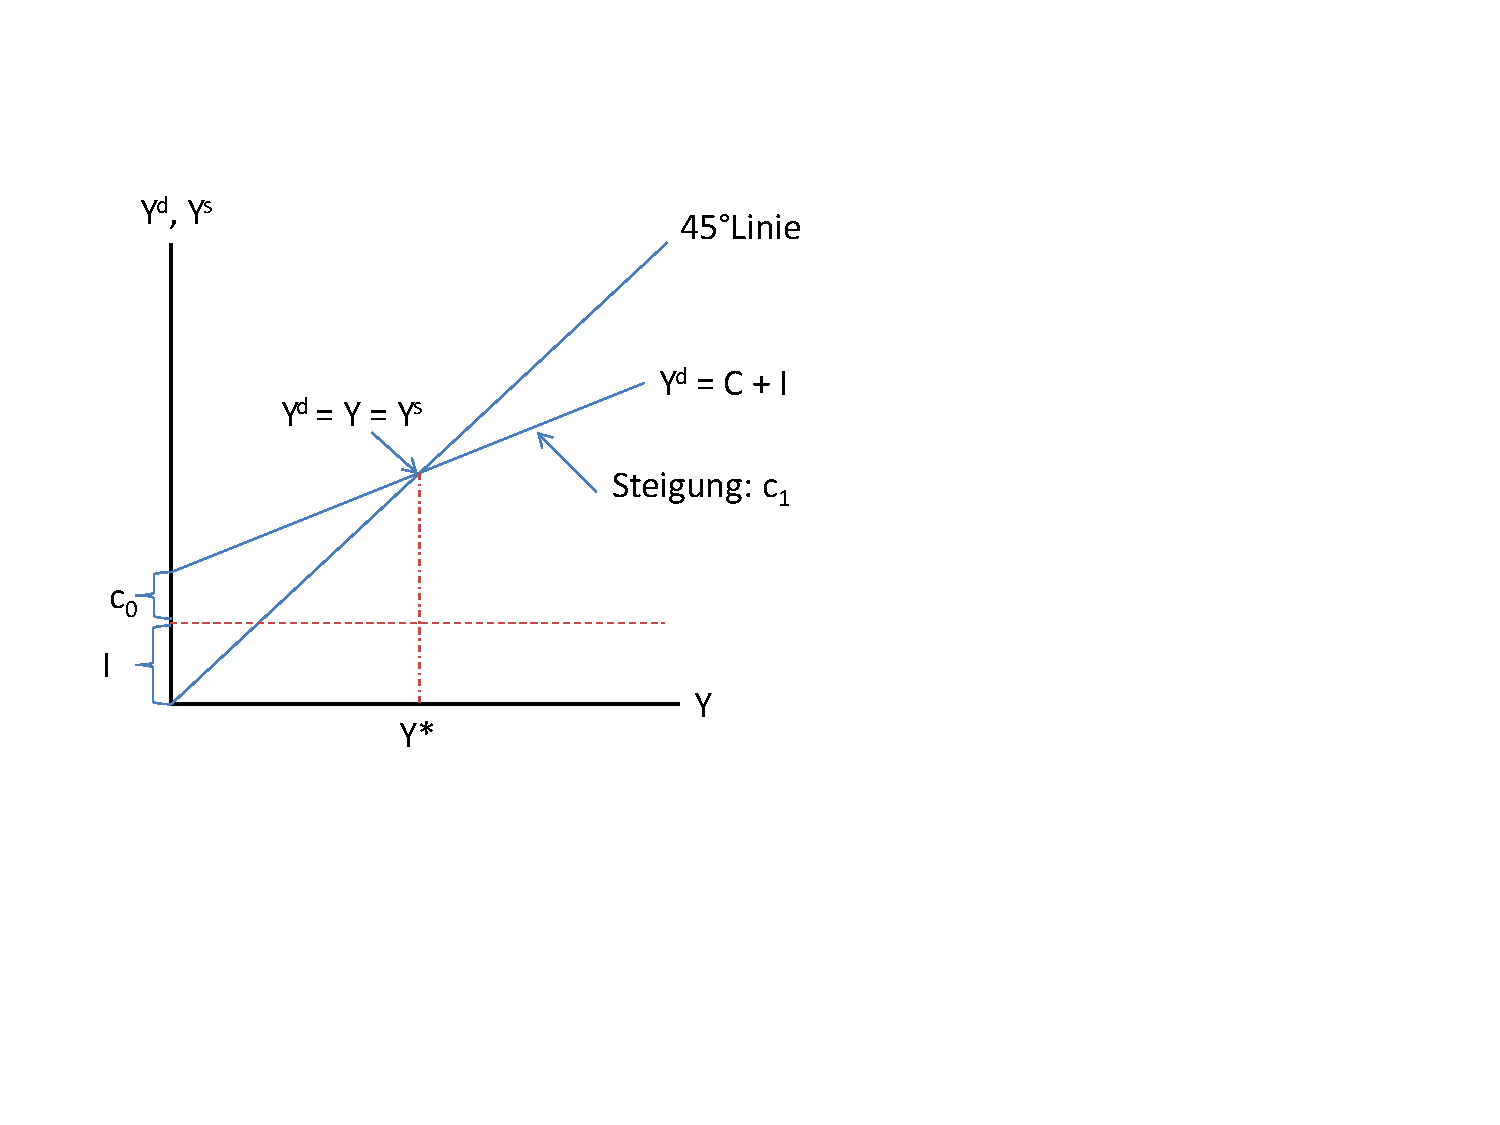
\includegraphics[width=.5\textwidth]{Bilder/Keynes_IS_GG1.pdf}
  \end{center}
  \item Sparfunktion
  \begin{align*}
    S=I \Leftrightarrow -C_{aut} + (1-c)Y = I_{aut} -b i\\
    Y= \frac{1}{1-c} (C_{aut} + I_{aut} - b i)
  \end{align*}
    \begin{center}
  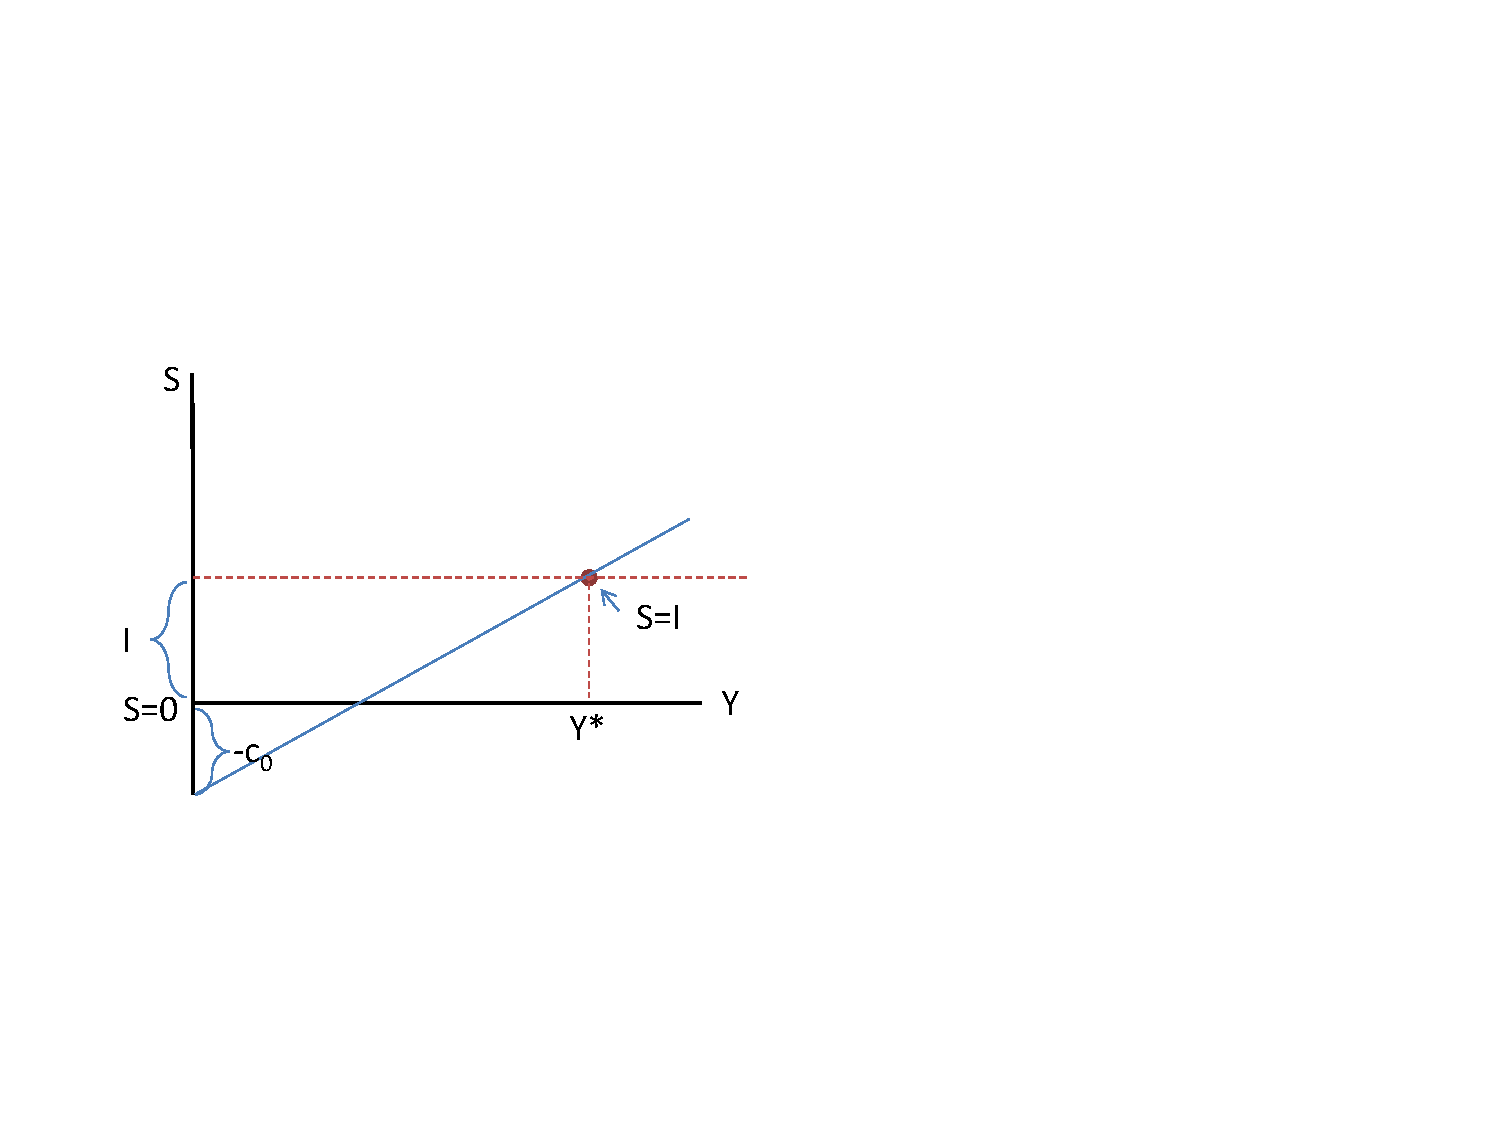
\includegraphics[width=.5\textwidth]{Bilder/Keynes_IS_GG2.pdf}
  \end{center}
\end{enumerate}
Sinnvolles Gleichgewicht existiert nur , wenn $0<c<1$, denn sonst ist $Y^* <0$.\\
\textbf{Vergleich zur (Neo-)Klassik:}\\Hier wird das GG \"{u}ber den Arbeitsmarkt und Produktionsfunktion bestimmt! Say: Jedes Angebot schafft sich seine Nachfrage vs. Keynes: Effektive Nachfrage

\item Erh\"{o}hung von $C_{aut}: \frac{\partial Y^*}{\partial C_{aut}}=\frac{1}{1-c}>1$
  \begin{itemize}
    \item Zunahme in $Y^*$ ist gr\"{o}{\ss}er als die urspr\"{u}ngliche Mehrnachfrage in $C_{aut}$
    \item Multiplikatorprozess!
  \end{itemize}

\textbf{Der Multiplikatorprozess:}
\begin{center}
  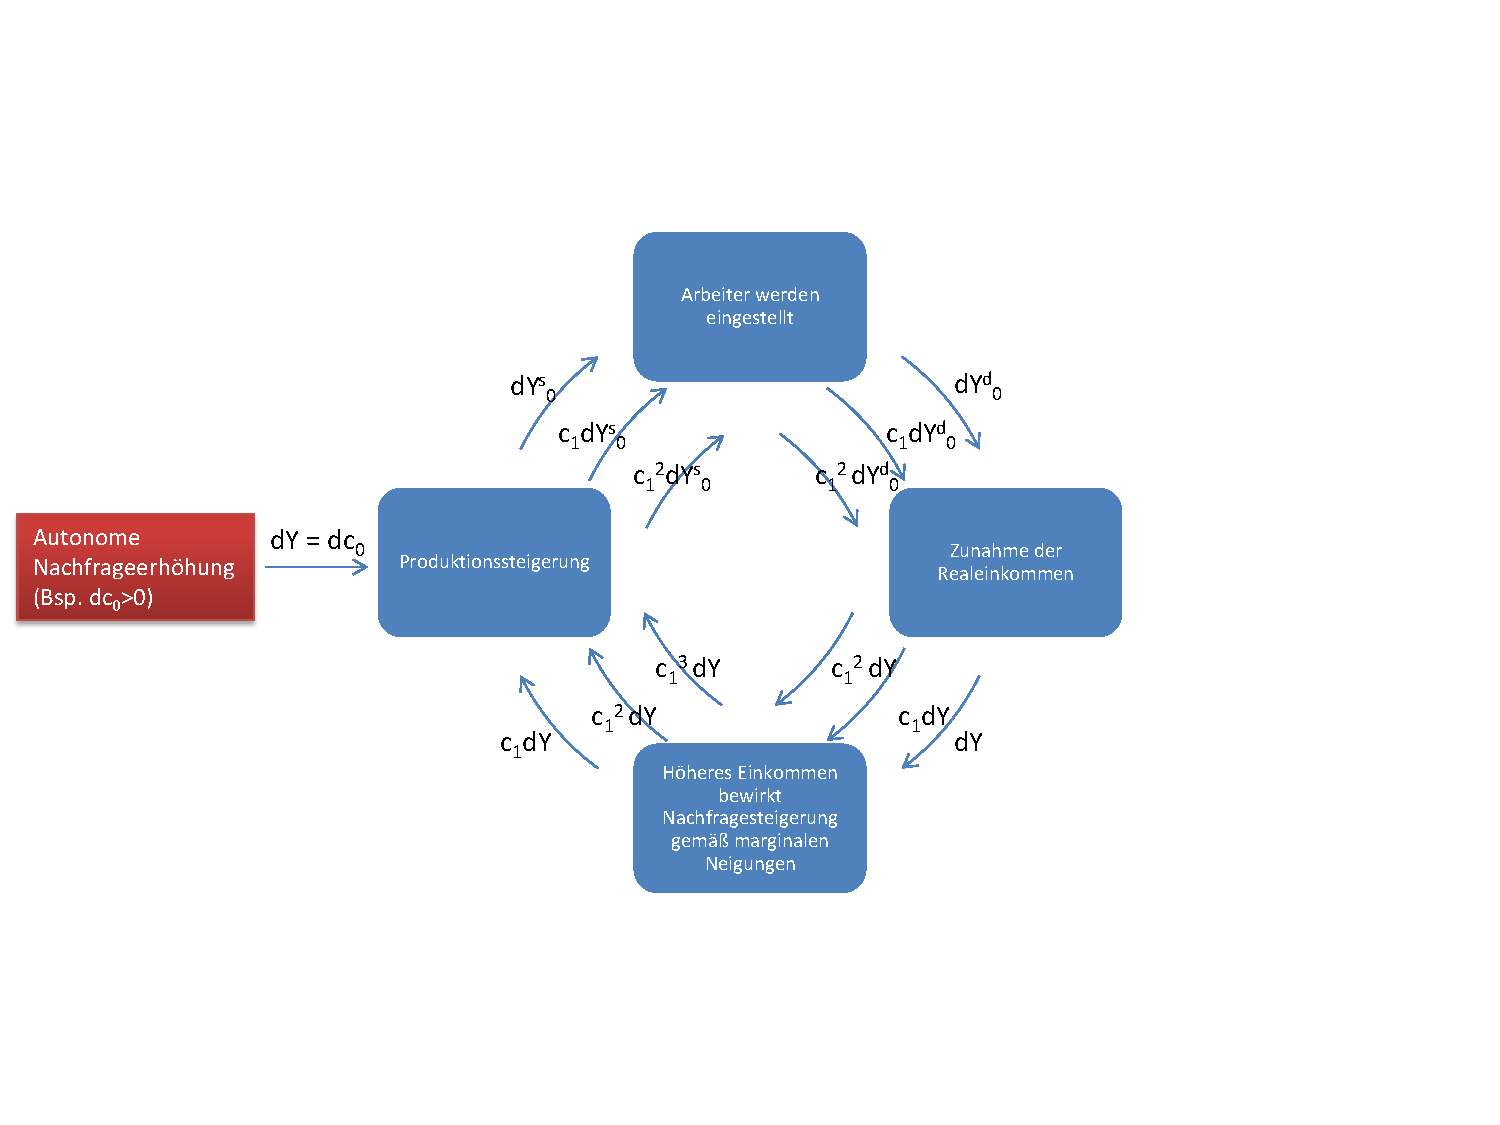
\includegraphics[width=\textwidth]{Bilder/Keynes_Multiplikator.pdf}
\end{center}
\begin{align*}
  d Y^* &= d C_{aut} + c d C_{aut} + c^2 d C_{aut} + \dots = d C_{aut} \cdot \overbrace{\underbrace{(1 + c + c^2+ \dots)}}_{=\frac{1}{1-c}, \text{falls } 0<c<1}^\text{Unendlichte geometrische Reihe}= \frac{1}{1-c}dC_{aut}, \\\text{ denn:}&\\
  d Y^* - c d Y^* &= d C_{aut}(1 + c + c^2+ \dots) - c d C_{aut}(1 + c + c^2+ \dots) \\
  &= d C_{aut} + d C_{aut}(c + c^2+ \dots) - d C_{aut}(c + c^2+ \dots) \\
  &= d C_{aut}\\
  \Leftrightarrow d Y^* &= \frac{d C_{aut}}{1-c}
\end{align*}
\begin{center}
  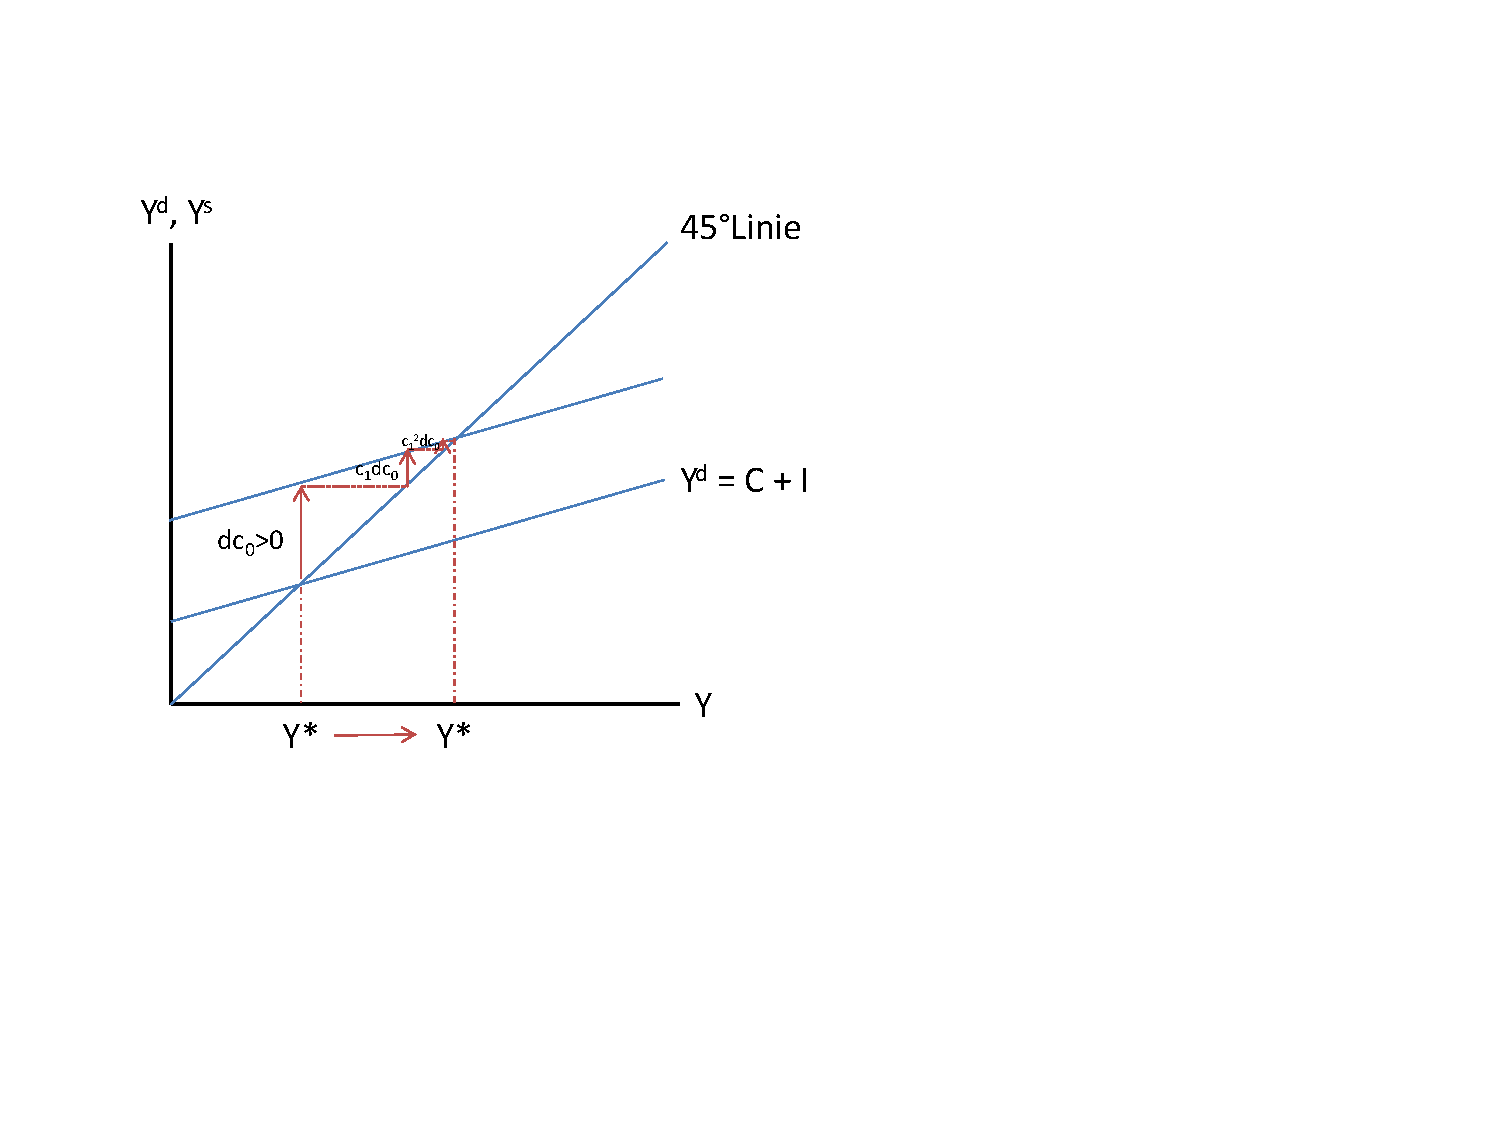
\includegraphics[width=0.5\textwidth]{Bilder/Keynes_Multiplikator_Grafisch.pdf}
\end{center}
\end{enumerate}

\subsection{Haavelmo Theorem im Keynesianischen Modell}
\begin{enumerate}
  \item $C=C_{aut}+c(Y-T)$ somit $Y=C+I+G=C_{aut}+cY-cT + I_{aut} + G \Leftrightarrow Y = \frac{1}{1-c}(C_{aut}-cT + I_{aut}+G)$
  \item Steuerfinanzierte Staatsausgabenerh\"{o}hung: $G=T$, d.h.
  $Y = \frac{1}{1-c}(C_{aut}-cG + I_{aut}+G)$ und somit $\frac{\partial Y}{\partial G}=\frac{1}{1-c} (1-c) = 1$. D.h. $dY=dG$ Expansive Wirkung ohne Budgetbelastung!\\ \textbf{Haavelmo Theorem:}\\
  Expanisve Wirkung das das Einkommen k\"{o}nnen von einem ausgeglichenem Staatshaushalt ausgehen (Mehr Steuer, diese Einnahmen sofort ausgeben). Grund: Staat besitzt im Gegensatz zu den privaten Haushalten keine marginale Sparquote, somit werden Steuereinnahmen zu 100\% Nachfragewirksam.\\
  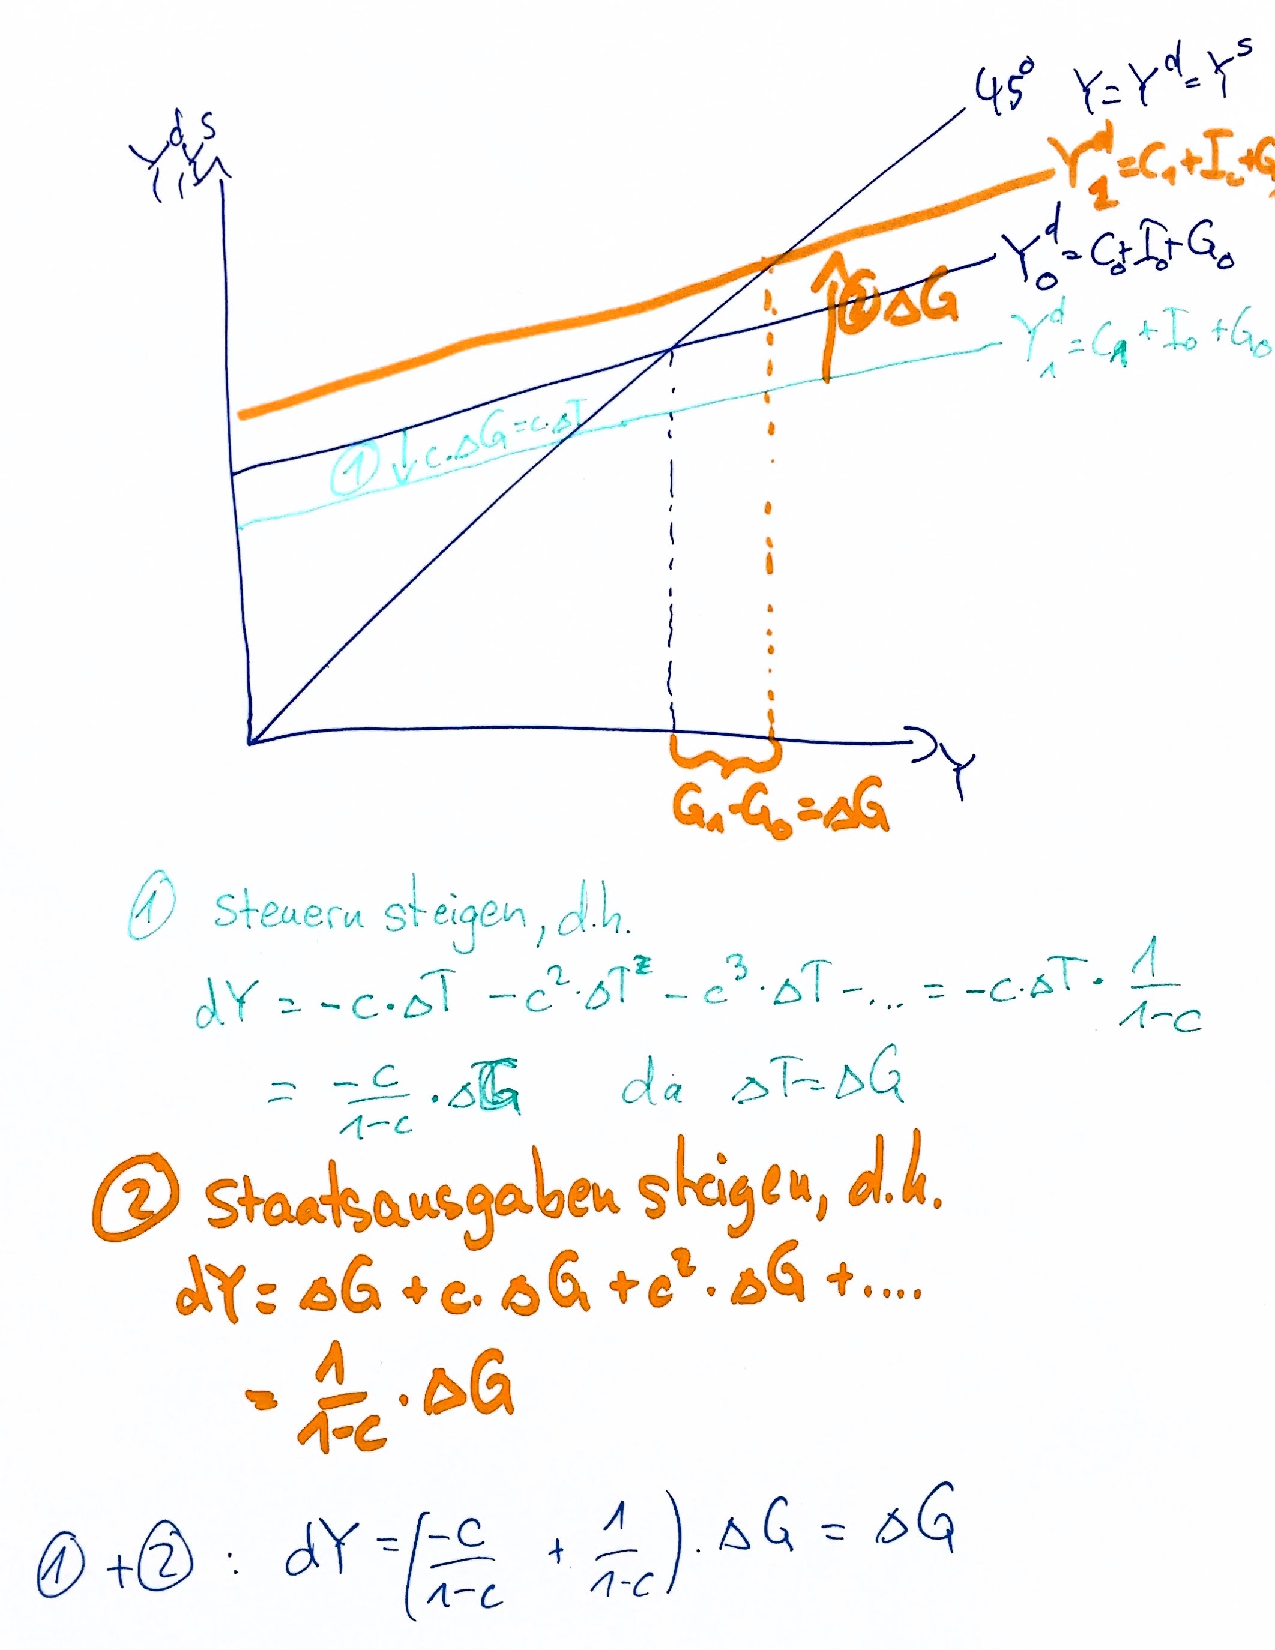
\includegraphics[width=.75\textwidth]{Bilder/Keynes_Haavelmo.pdf}
\end{enumerate}

\subsection{G\"{u}termarkt und IS-Kurve}
\begin{enumerate}[(a)]
\item \textbf{IS-Kurve Analytisch:}
\begin{itemize}
\item Berechnung der Sparfunktion:
\begin{align*}
  S &= S^{Pr} + S^{St} = (Y-C-T) + (T-G) = Y-C_{aut} -c\underbrace{(Y-T_{aut} - q Y)}_{\equiv Y^v} - G_{aut}\\
  \Leftrightarrow S&= -G_{aut} - C_{aut} - c T_{aut} + (1-c(1-q))Y
\end{align*}
\item $I(i)=S(Y):$
\begin{align*}
  I_{aut} - b i &= -G_{aut} - C_{aut} - c T_{aut} + (1-c(1-q))Y\\
  \Leftrightarrow Y &= \frac{1}{1-c(1-q)}(C_{aut} - c T_{aut} + I_{aut} + G_{aut} - b i)\\
  \Leftrightarrow i &=\frac{1}{b}(C_{aut} -c T_{aut} + G_{aut} - (1-c(1-q))Y)
\end{align*}
\end{itemize}

\textbf{IS-Kurve Grafisch:}
\begin{center}
  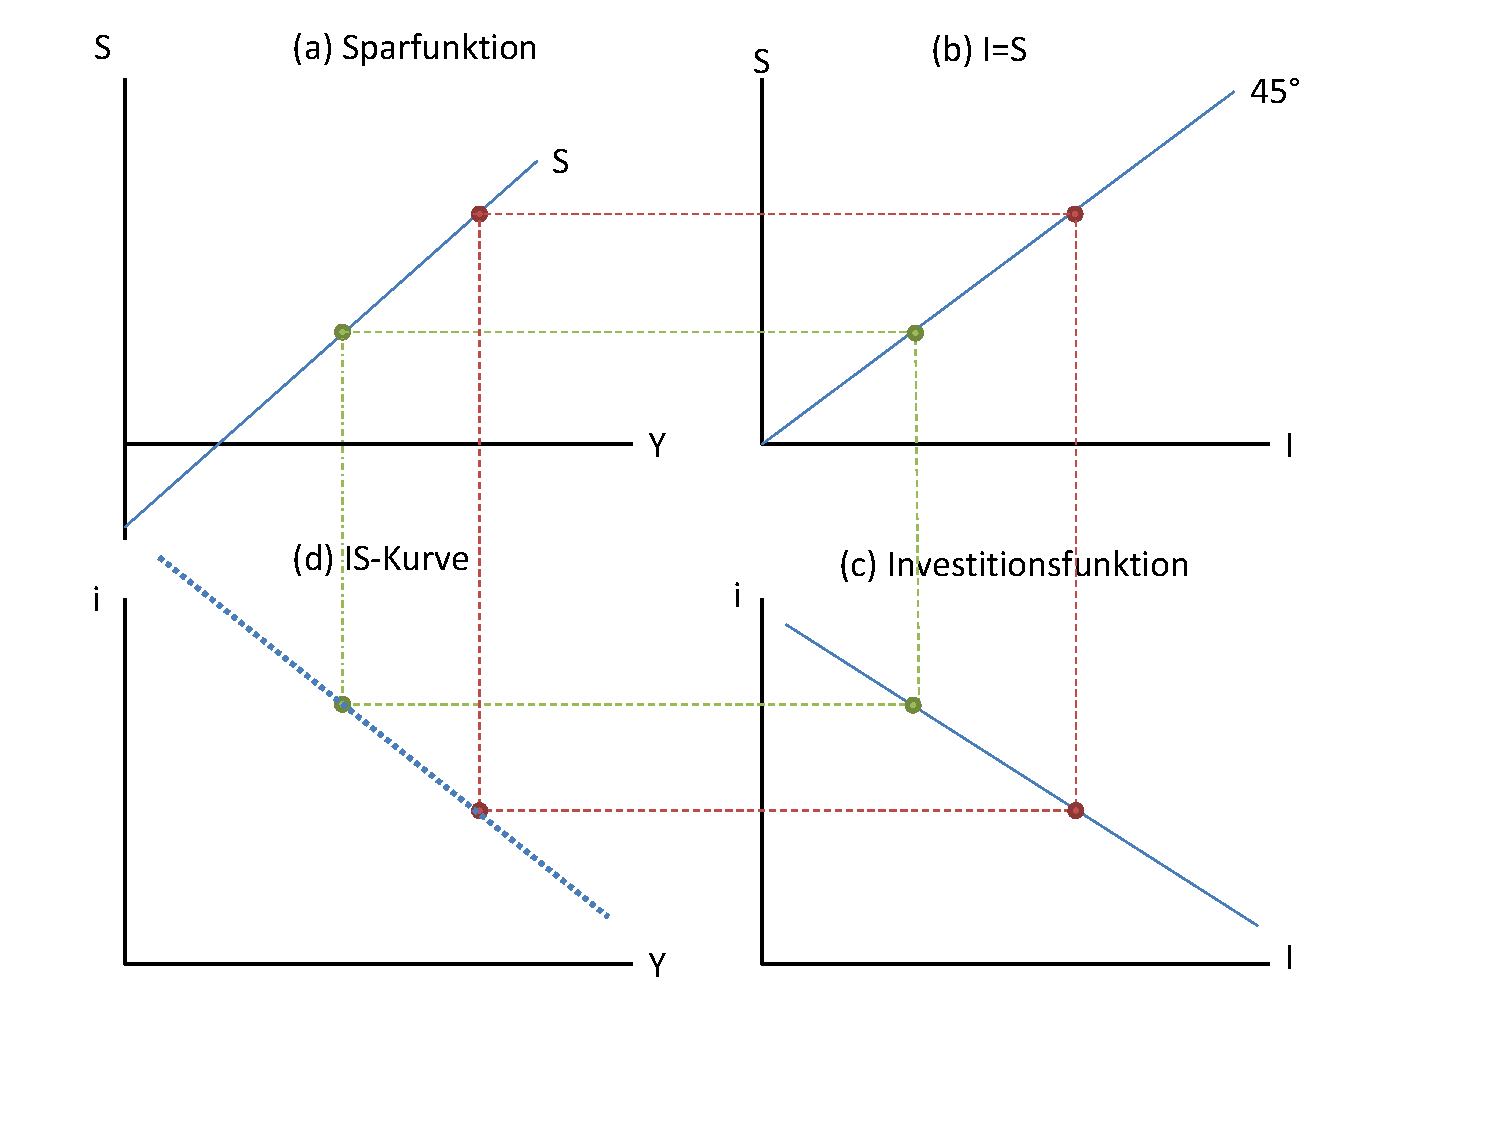
\includegraphics[width=\textwidth]{Bilder/Keynes_IS_Grafisch.pdf}
  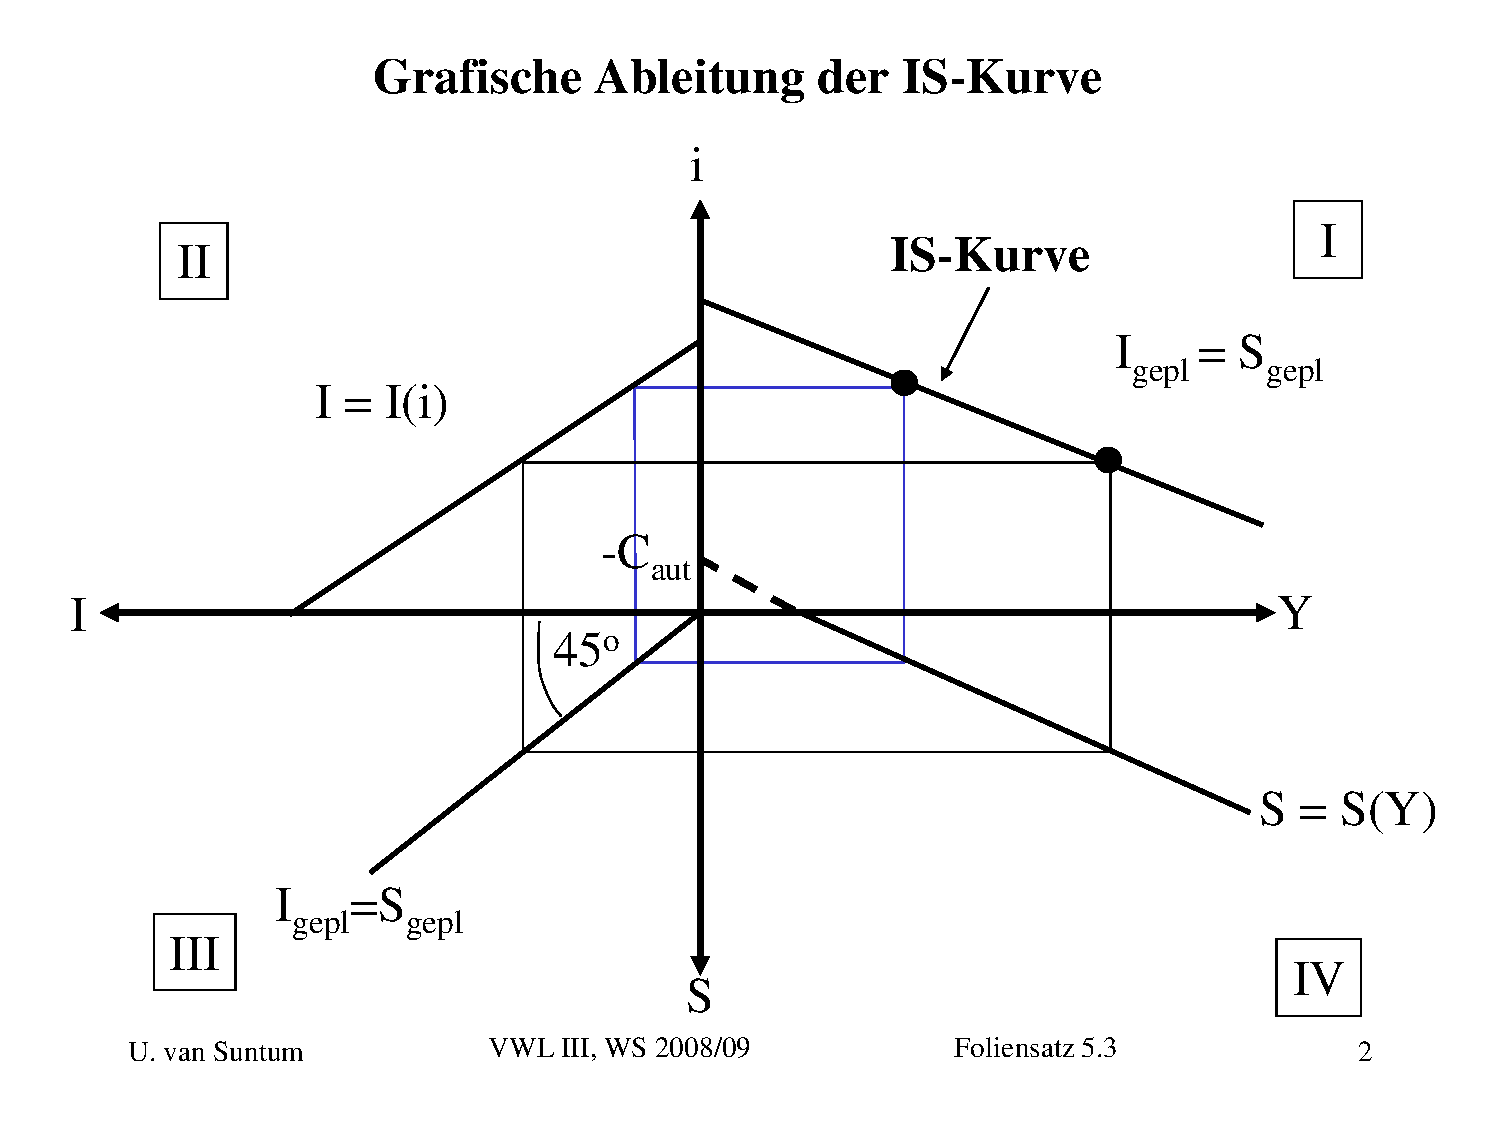
\includegraphics[width=\textwidth]{Bilder/Keynes_IS_Grafisch2.pdf}
\end{center}
IS-Kurve ordnet jedem Zinssatz ein gleichgewichtiges Einkommen zu.\\
Idee: Jedem Zinssatz ist eine Investitionsnachfrage zugeordnet. Wie hoch muss Y sein, damit die Ersparnis in H\"{o}he der Investitionsnachfrage entsteht.\\
Logik f\"{u}r negative Zinsabh\"{a}ngigkeit vom Zins:\\
Wenn i steigt, sinken die Investitionen. Da diese Bestandteil der effektiven Nachfrage sind, sinkt das Einkommen $Y^*$.\\

\item
\textbf{Steigung der IS-Kurve:}
\begin{align*}
  \frac{\partial i}{\partial Y} = -\frac{1}{b}(1-c(1-q))<0
\end{align*}
Interpretation:
\begin{itemize}
  \item Wie stark muss der Zins fallen damit eine Erh\"{o}hung von $Y^*$ um eine marginale Einheit m\"{o}glich ist
  \item $i\downarrow \rightarrow I\uparrow\rightarrow Y \uparrow$
  \item Alternativ: Wie stark muss das Einkommen steigen, damit bei einer Senkung der Zinsen um ein marginales Prozent wieder das Gleichgewicht auf dem G\"{u}termarkt erreicht wird.
\end{itemize}
\textbf{Steigungsparameter:}
\begin{itemize}
\item Zinsabh\"{a}ngigkeit von I (Betrachte relativ gro{\ss}es $b$):
\begin{itemize}
  \item $i\downarrow$
  \begin{itemize}
  \item[$\rightarrow$] starke Erh\"{o}hung von I
  \item[$\rightarrow$] starke Erh\"{o}hung von Y n\"{o}tig, um $S(Y)=I(i)$ wiederherzustellen
  \item[$\rightarrow$] Flache IS-Kurve
  \end{itemize}
\end{itemize}
\item Marginale Konsumneigung (Betrachte relativ hohes $c$) [Marginale Sparquote ist s=1-c]:
\begin{itemize}
  \item $i\downarrow\rightarrow I\uparrow \rightarrow Y\uparrow \rightarrow S(Y) \uparrow$
  \item Bei hohem $c$ gilt, dass h\"{o}heres Y zu geringerer zus\"{a}tzlicher Ersparnis f\"{u}hrt
  \item Multiplikator ist bei hohem $c$ gro{\ss}
  \item Flache IS-Kurve
\end{itemize}
\item Steuersatz q (Betrachte relativ hohes q)
\begin{itemize}
  \item Wenn q hoch ist, ist eine geringe Vergr\"{o}{\ss}erung von Y n\"{o}tig, damit $S=I$ wiederhergestellt ist
  \item IS-Kurve verl\"{a}uft steiler fallend
\end{itemize}
\end{itemize}
\textbf{Lageparameter:}
\begin{itemize}
  \item $C_{aut} \uparrow, I_{aut} \uparrow, G_{aut} \uparrow \rightarrow $ Bei gegebenem $i$ f\"{u}hrt dies zu h\"{o}herem Y gem\"{a}{\ss} Multiplikatorprozess
  \item[$\hookrightarrow$] IS-Kurve verschiebt sich nach RECHTS!
  \item $T_{aut}\uparrow \rightarrow C\downarrow, Y\downarrow$ bei gegebenem i $\rightarrow$ R\"{u}ckgang G\"{u}ternachfrage
    \item[$\hookrightarrow$] IS-Kurve verschiebt sich nach LINKS!
\end{itemize}
Zusammenfassend: Steuererh\"{o}hungen wirken kontraktiv, Erh\"{o}hung der autonomen Nachfragekomponenten wirken expansiv!

\item
IS-Kurve bildet das \textbf{simultane} Gleichgewicht auf dem G\"{u}termarkt und dem Kapitalmarkt ab, denn auf dem G\"{u}termarkt ist die geplante Nachfrage gleich dem realisierten Einkommen, w\"{a}hrend auf dem Kapitalmarkt geplante Investitionen im Gleichgewicht der geplanten Ersparnis entsprechen!
\end{enumerate}


\subsection{Geldmarkt und LM-Kurve}
\begin{enumerate}[(a)]
    \item LM-Kurve: Reale Geldnachfrage = Reales Geldangebot: $(L(\overset{+}{Y},\overset{-}{i})=\frac{M}{P})$
    \begin{enumerate}[(i)]
    \item Geldnachfrage (real): $L(\overset{+}{Y},\overset{-}{i})$
    \begin{itemize}
      \item Transaktionsmotiv:
      \begin{itemize}
      \item Mehr Einkommen $\rightarrow$ Mehr K\"{a}ufe $\rightarrow$ Mehr Geld wird ben\"{o}tigt, d.h. $L_T=L_T(\overset{+}{Y})$, positiv abh\"{a}ngig von Y.
      \end{itemize}
      \item Vorsichtsmotiv:
      \begin{itemize}
      \item Transaktionsbedarf nur begrenzt vorhersehbar
      \item Halte mehr Geld als zu Transaktionszwecken im Durchschnitt n\"{o}tig
      \item Ausgabenschwankungen nehmen mit Ausgaben zu, d.h. $L_V=L_V(\overset{+}{Y})$
      \end{itemize}
      \item Spekulationsmotiv (HIER NOCH GENAUER):
        \begin{itemize}
          \item Geld halten statt Wertpapiere, da Kursver\"{a}nderungen mit ber\"{u}cksichtigt werden.
          \item Grundidee: Kapitalmarkt und Wertpapiermarkt stehen in Konkurrenz, Zins verbindet sie
          \begin{itemize}
          \item Kapitalmarkt: $I=S, dB^s=dB^d$ Bondneuemission
          \item Wertpapiermarkt: Alte Bonds werden gehandelt
          \item Verzinsung muss aber identisch sein
          \end{itemize}
          \item Bei uns: Kapitalmarkt wird \"{u}ber G\"{u}termarkt abgebildet und Wertpapiermarkt \"{u}ber Geldmarkt. Da beide zusammenwirken, folgt identischer Zins.
          \item $i\uparrow$, d.h. mehr Leute glauben, dass Zins und Kursver\"{a}nderungen eines Wertpapiers gr\"{o}{\ss}er als Null sind und wollen mehr Wertpapiere als Geld halten $\rightarrow L_S=L_S(\overset{-}{i})$
        \end{itemize}
        \item Somit: $L = L_T(\overset{+}{Y})+L_V(\overset{+}{Y})+L_S(\overset{-}{i}) = L(\overset{+}{Y},\overset{-}{i})$
    \end{itemize}

    \item Geldangebot (nominal), $M^s=M$
    \begin{itemize}
      \item Exogen gegeben, da von Zentralbank kontrolliert!
      \item Wie macht die Zentralbank das?
      \begin{itemize}
      \item Offenmarktpolitik [bzw. evtl. durch Mindestreservesatz]
      \item Offenmarktpolitik: Ankauf oder Verkauf von Wertpapieren (bzw. Repos)
      \item Idee:
      \begin{itemize}
        \item ZB kauft Wertpapiere, bezahlt mit Geld $(M\uparrow)$
        \item ZB verkauft Wertpapiere, bekommt Geld $(M\downarrow)$
      \end{itemize}
      \item Genauer: Negativer Zusammenhang zwischen Kurs und aktuellem Zins eines Wertpapiers aufgrund von Arbitrage:
      \begin{align*}
        (1+i)P_B = \underbrace{NW\cdot(1+i_0)}_\text{konstant}
      \end{align*}
      \item D.h. wenn ZB Wertpapiere nachfragt, steigt $P_B$, da $NW\cdot(1+i_0)$ konstant ist, muss $i$ sinken: $P_B\uparrow \rightarrow i \downarrow$
      \item Bei gegebenem $Y$ folgt $i\downarrow \rightarrow L(Y,\overset{-}{i})\uparrow$, da $\frac{\partial L}{\partial i}<0$. Daraus folgt $M\uparrow$.
      \item In der Realit\"{a}t ist die Zentralbank aber nur begrenzt f\"{a}hig, $M$ zu steuern aufgrund der Geldsch\"{o}pfung der Gesch\"{a}ftsbanken
      \end{itemize}
    \end{itemize}
    \item Gleichgewicht: $M^s=M^d $
    \begin{align*}
      \Leftrightarrow \underbrace{\frac{M}{P}}_\text{konstant}=L(\overset{+}{Y},\overset{-}{i})
    \end{align*}
    \begin{itemize}
      \item Aufgrund des exogenen Geldangebots muss auch die Geldnachfrage konstant sein!
      \item Wenn Y steigt, muss i auch steigen! $\rightarrow$ Positive Steigung der LM-Kurve!
      \item $Y\uparrow\rightarrow (L_T+L_V)\uparrow$, d.h. Subjekte brauchen mehr Geld, also wollen sie Wertpapiere verkaufen $\rightarrow P_B \downarrow \rightarrow i \uparrow \rightarrow L_i \downarrow$, d.h. Wertpapierkauf wird immer unattraktiver und die Geldnachfrage kehrt zum urspr\"{u}nglichen Niveau zur\"{u}ck.
    \end{itemize}
  \end{enumerate}
  \item Geldmarkt:
  \begin{center}
  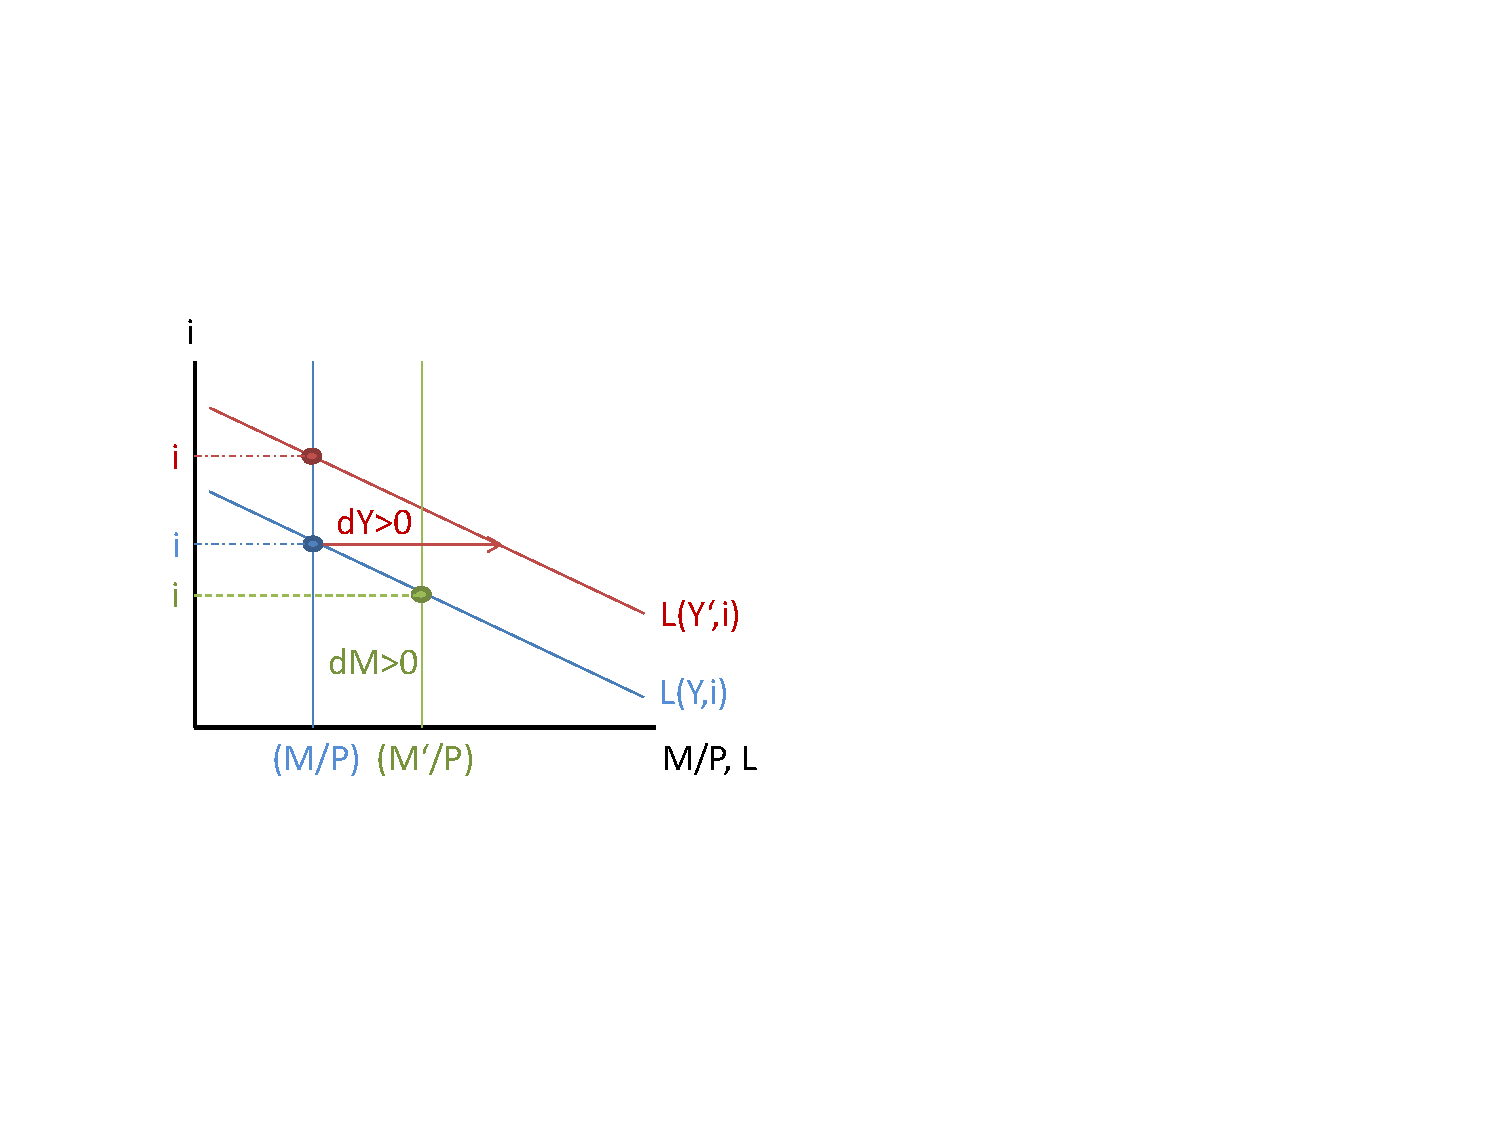
\includegraphics[width=.5\textwidth]{Bilder/Keynes_Geldmarkt.pdf}
  \end{center}
  Ver\"{a}nderungen:
  \begin{itemize}
    \item $Y \uparrow \rightarrow$ Rechtsverschiebung der Geldnachfrage, d.h. $i\uparrow$
    \item $M\uparrow$ bzw. $P \downarrow \rightarrow$ Rechtsverschiebung des Geldangebots, d.h. $i \downarrow$
  \end{itemize}
  \item Herleitung LM-Kurve:
  \begin{itemize}
    \item Grafisch:
  \begin{center}
  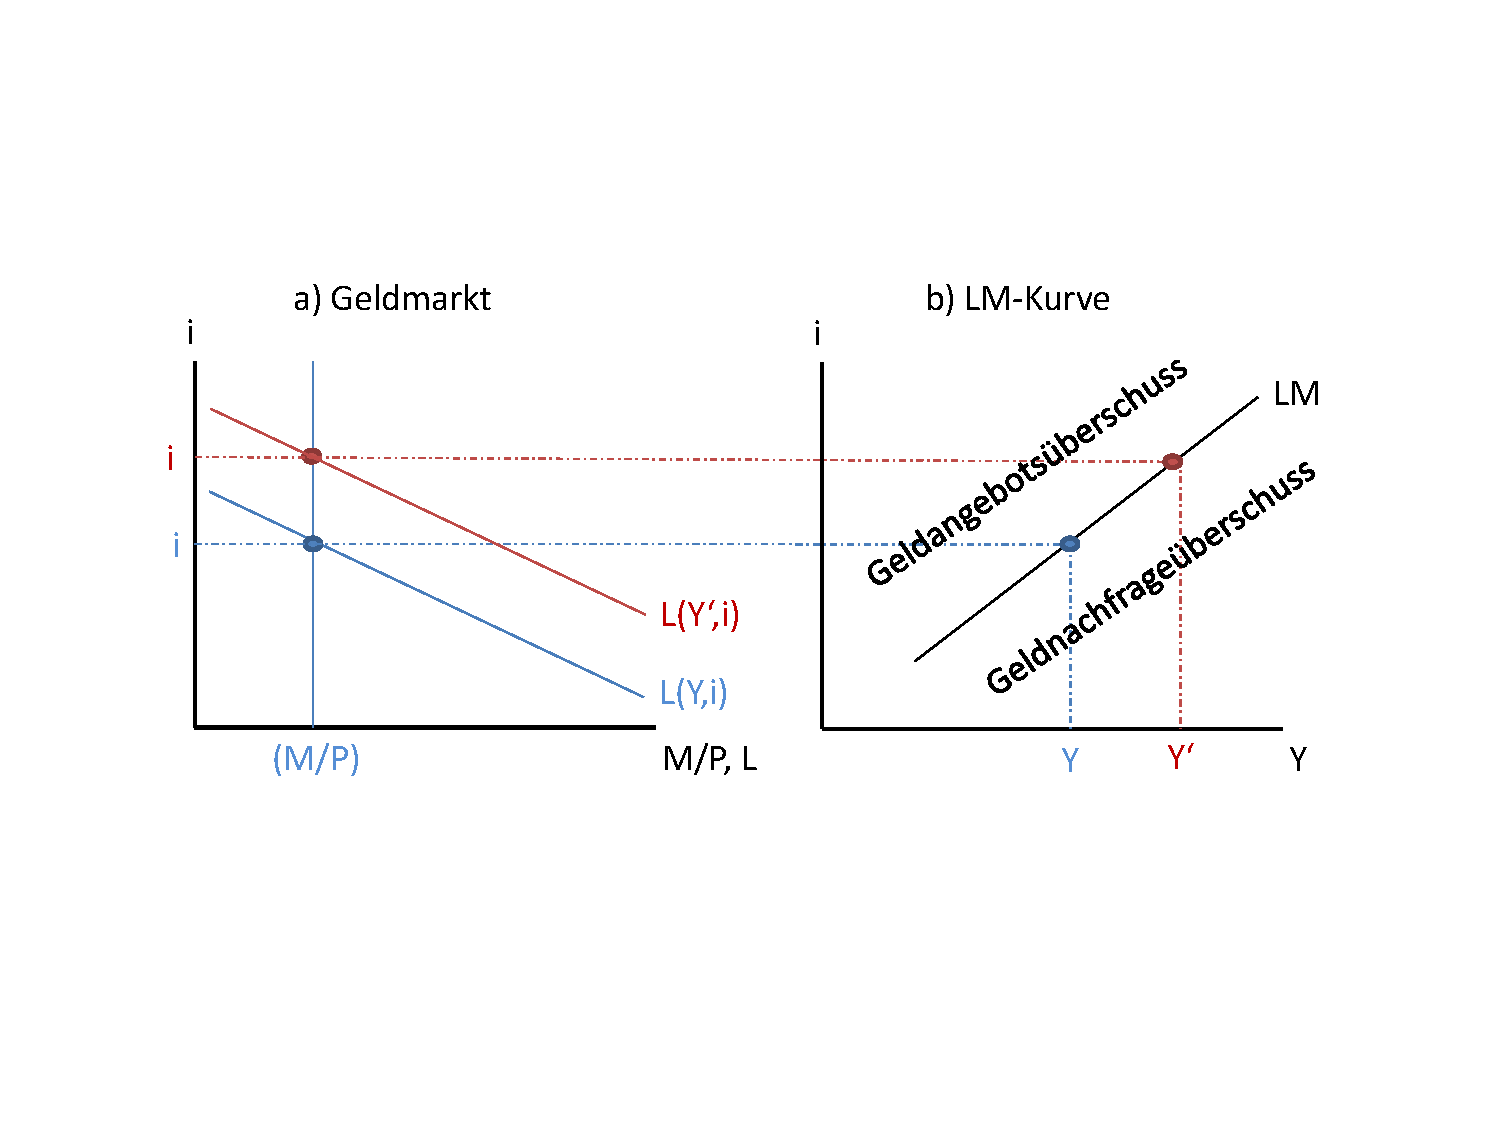
\includegraphics[width=\textwidth]{Bilder/Keynes_LM.pdf}\\
    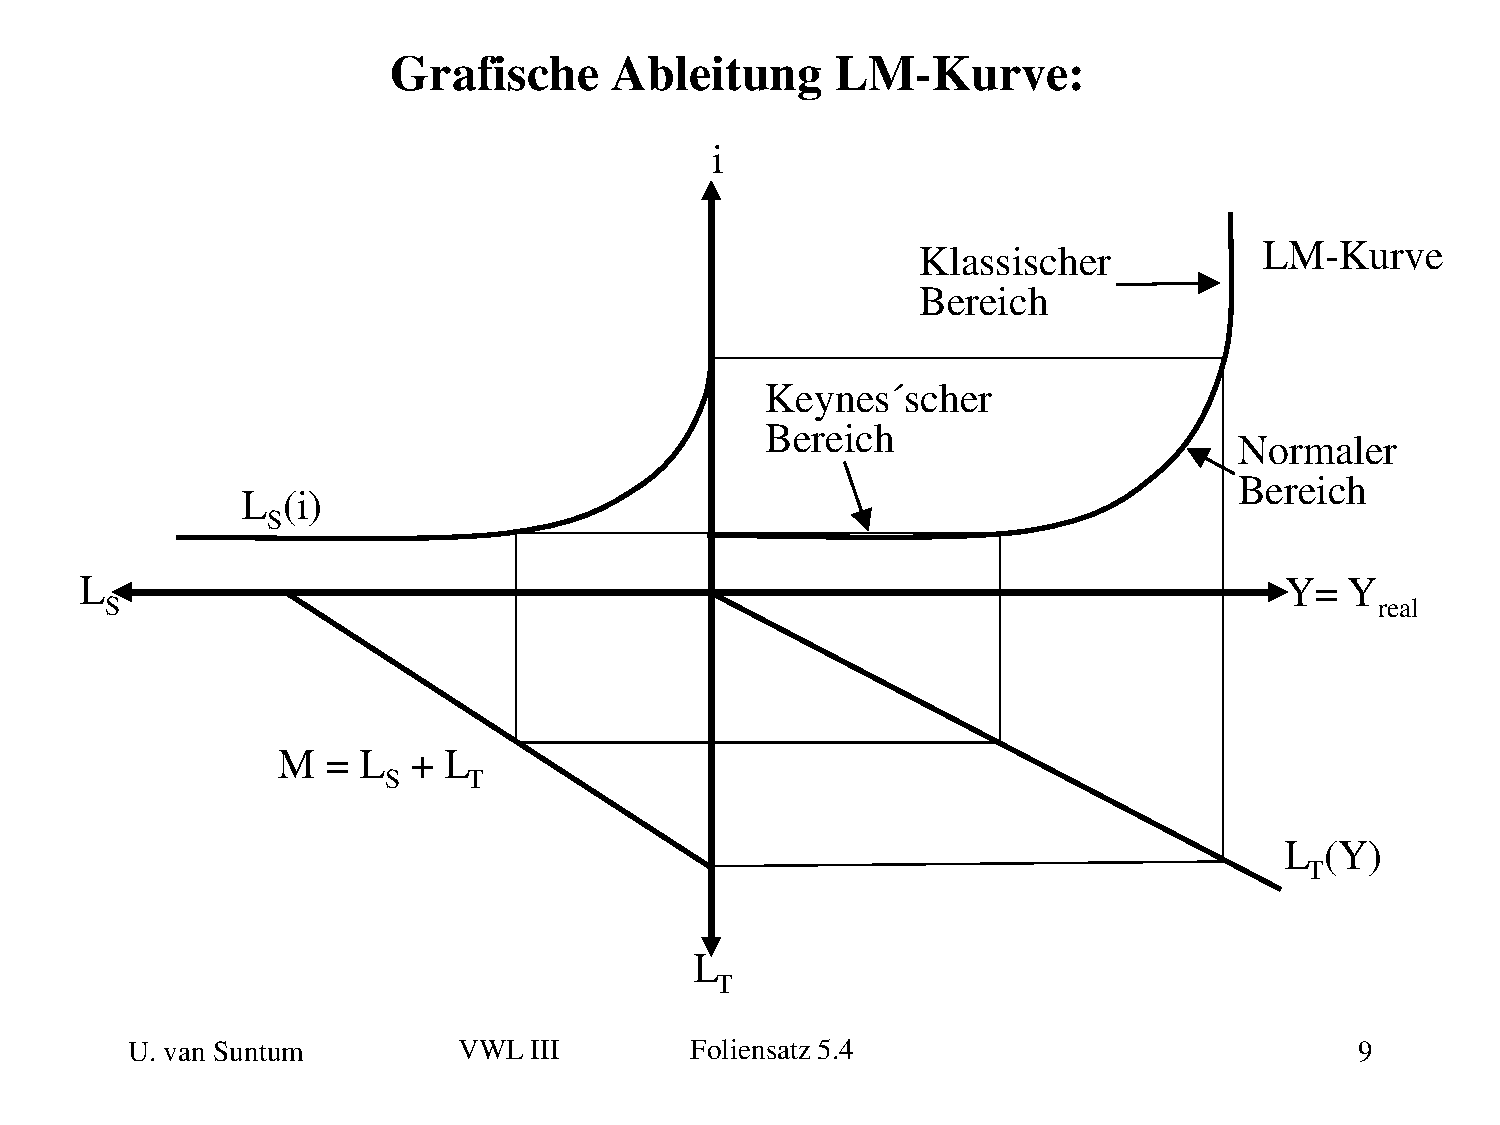
\includegraphics[width=\textwidth]{Bilder/Keynes_LM2.pdf}
  \end{center}
    \item Analytisch:
    \begin{align*}
      \frac{M}{P}= L(Y,i)
    \end{align*}
    Hier kommt es auf die funktionale Form von L an, einfach nach Y oder i aufl\"{o}sen.
  \end{itemize}
  \item
  \begin{itemize}
    \item Steigung:
  \begin{align*}
    \frac{M}{P}&= L(Y,i)\\
    \frac{1}{P}dM - \frac{M}{P^2}dP &= \overset{>0}{L_Y} dY + \overset{<0}{L_i} di
  \end{align*}
  F\"{u}r Steigung: $dM=dP=0$:
  \begin{align*}
    \frac{dY}{di}=-\frac{L_Y}{L_i}>0
  \end{align*}
   \item Zinsabh\"{a}ngigkeit von L, betrachte also $L_i$:
   \begin{itemize}
     \item hohes $|L_i| \rightarrow$ Flacher Verlauf der  LM-Kurve
     \item niedriges $|L_i| \rightarrow$ Steiler Verlauf der LM-Kurve
     \item Klassik: $L_i=0 \rightarrow$ Senkrechte LM-Kurve
     \item Liquidit\"{a}tsfalle $L_i= -\infty \rightarrow$ horizontale LM-Kurve
   \end{itemize}
   \item Einkommensabh\"{a}nigkeit der Geldnachfrage, betrachte also $L_Y$
   \begin{itemize}
     \item Hohes $L_Y, Y\uparrow \rightarrow L\upuparrows$, d.h. starke Zinserh\"{o}hung erforderlich, um Geldnachfrage wieder auf das Niveau der realen Geldmenge zu bringen $\rightarrow$ Steile LM-Kurve
   \end{itemize}
   \item Lageparameter (Verschiebung der LM-Kurve)
   \begin{align*}
       \frac{1}{P}dM - \frac{M}{P^2}dP &= \overset{>0}{L_Y} dY + \overset{<0}{L_i} di
       \end{align*}
  \begin{itemize}
     \item Erh\"{o}hung von $M (di=dP=0)$
     \begin{align*}
       \frac{dY}{dM}=\frac{1}{P L_Y} >0
     \end{align*}
     $\rightarrow$ Rechstverschiebung, zu jedem Outputniveau ist nun ein h\"{o}heres Zinsniveau erforderlich
     \item Erh\"{o}hung von $P (di=dM=0)$
     \begin{align*}
       \frac{dY}{dP}=\frac{-M}{P^2 L_Y} <0
     \end{align*}
     $\rightarrow$ Linksverschiebung
   \end{itemize}
  \end{itemize}
  \item LM-Kurve ist der geometrische Ort aller Kombinationen aus Zinsen und Einkommen, f\"{u}r die der Geldmarkt im Gleichgewicht ist.
\end{enumerate}

\subsection{Wirtschaftspolitische Ma{\ss}nahmen}
\begin{enumerate}
\item Herleitung IS (G\"{u}termarkt-GG):
\begin{align*}
  Y^d=Y^s=Y &= C+I+G = C_{aut} + c(Y-T_{aut}) + I_{aut}-bi + G_{aut}\\
  Y &= \frac{1}{1-c}(C_{aut} - cT_{aut} + I_{aut}-bi + G_{aut})\\
  \text{Totales Differential:}\\
  dY &= \frac{1}{1-c}(dC_{aut}-c dT_{aut} + dI_{aut} - b di + dG_{aut})
\end{align*}

\item Herleitung LM (Geldmarkt-GG):
\begin{align*}
  M = M^a = P L \Leftrightarrow \frac{M}{P} &= L(Y,i) = lY-ki\\
  i =\frac{-1}{k}\left(\frac{M}{P}-lY\right)\\
  \text{Totales Differential:}\\
  \frac{1}{P}dM - \frac{M}{P^2}dP &= L_Y dY + L_i di\\
  \Leftrightarrow di &= \frac{1}{L_i} \left(\frac{1}{P}dM-\frac{M}{P^2}dP-L_Y dY\right)
\end{align*}
\item LM in IS einsetzen, und Terme zusammenfassen
\begin{align*}
  Y = \frac{1}{1-c +\frac{b l}{k}} \left(C_{aut} - c T_{aut} + I_{aut} +G_{aut} + \frac{b}{k} \frac{M}{P}\right)
\end{align*}
oder in totalem Differential
\begin{align*}
  dY = \frac{1}{1-c -\frac{b L_Y}{L_i}} \left(dC_{aut} - c dT_{aut} + dI_{aut} +dG_{aut} - \frac{b}{L_i} \left(\frac{1}{P}dM-\frac{M}{P^2}dP\right)\right)
\end{align*}
Positive Einflussfaktoren: $C_{aut}$, $I_{aut}$, $G_{aut}$, $M$\\
Negative Einflussfaktoren: $T_{aut}$, $P$

\item
\begin{enumerate}
  \item Steuerfinanzierte Staatsausgabenerh\"{o}hung
  \begin{align*}
    G_{aut}&=T_{aut}>0;\\
  \frac{dY}{dG} &= \frac{1}{1-c +\frac{b l}{k}} \left(- c +1 \right) = \frac{\overbrace{1-c}^{>0}}{\underbrace{\overbrace{1-c}^{>0} + \frac{b l}{k}}_{>0}} >0\\
  \frac{di}{dG} &= \underbrace{\frac{l}{k}}_{>0} \underbrace{\frac{dY}{dG}}_{>0} >0
  \end{align*}
  \begin{align*}
    dG_{aut}&=dT_{aut}>0; dM_{aut}=dI_{aut}=dC_{aut}=dP=0, P=1\\
  dY &= \frac{1}{1-c -\frac{b L_Y}{L_i}} \left(- c \underbrace{dT_{aut}}_{=dG_{aut}} +dG_{aut} \right) = \frac{\overbrace{1-c}^{>0}}{\underbrace{\overbrace{1-c}^{>0} - \overbrace{\frac{b L_Y}{L_i}}^{<0}}_{>0}} \underbrace{dG_{aut}}_{>0} >0\\
  di &= \underbrace{\frac{-L_Y}{L_i}}_{>0} \underbrace{dY}_{>0} >0
  \end{align*}
  Eine Steuerfinanzierte Staatsausgabenherh\"{o}hung erh\"{o}ht Y und i --> Expansive Wirkung\\
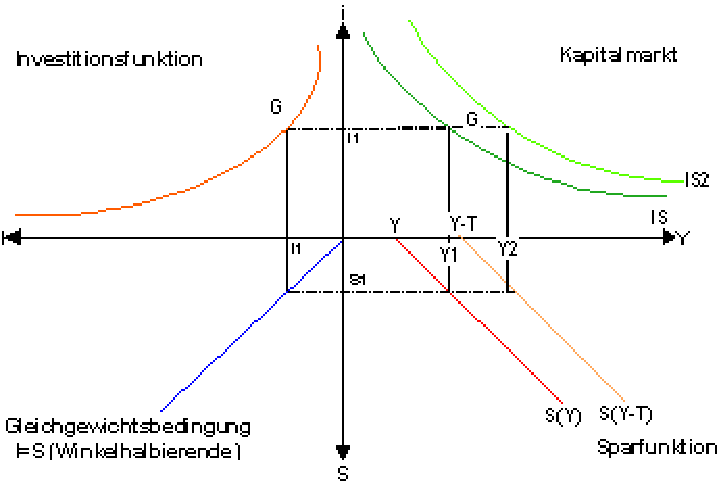
\includegraphics[width=0.5\textwidth]{Bilder/Keynes_IS_LM_Steuerfinanziert.pdf}\\
Durch Steuern wird die Sparfunktion um T(=G) verschoben; Bei einem konstanten Zins $i_1$ und einer Konstanten Sparleistung $S_1$ mu{\ss} sich jetzt das Einkommen erh\"{o}hen von $Y_1$ auf $Y_2$. Daher verschiebt sich die IS-Kurve genau um G nach au{\ss}en und das Einkommen steigt ebenfalls um $G=Y_2-Y_1$. Grund der Einkommenssteigerung ist die marginale Konsumneigung.\\
Fazit: Kampf gegen Arbeitslosigkeit m\"{o}glich ohne Budgetbelastung!
Haavelmo Theorem!

\item Kreditfinanzierte Steuersenkung
  \begin{align*}
    dT&<0\\
  \frac{dY}{dT} &= \frac{1}{1-c +\frac{b l}{k}} \left(- c \right) <0\\
  \Leftrightarrow dY &= \frac{-c}{1-c +\frac{b l}{k}} \underbrace{dT}_{<0} >0\\
  \frac{di}{dT} &= \frac{l}{k} \frac{dY}{dT} <0\\
  \Leftrightarrow di &= \frac{l}{k} dY > 0
  \end{align*}
  \begin{align*}
    dT_{aut}&<0; dM_{aut}=dI_{aut}=dC_{aut}=dG_{aut}=dP=0, P=1\\
  dY &= \frac{1}{1-c -\frac{b L_Y}{L_i}} \left(- c \underbrace{dT_{aut}}_{<0}\right) >0\\
  di &= \frac{-L_Y}{L_i} dY >0
  \end{align*}
  Eine Kreditfinanzierte Steuersenkung erh\"{o}ht Y und i; Wirkung umso st\"{a}rker, je h\"{o}her die marginale Konsumneigung ist.\\
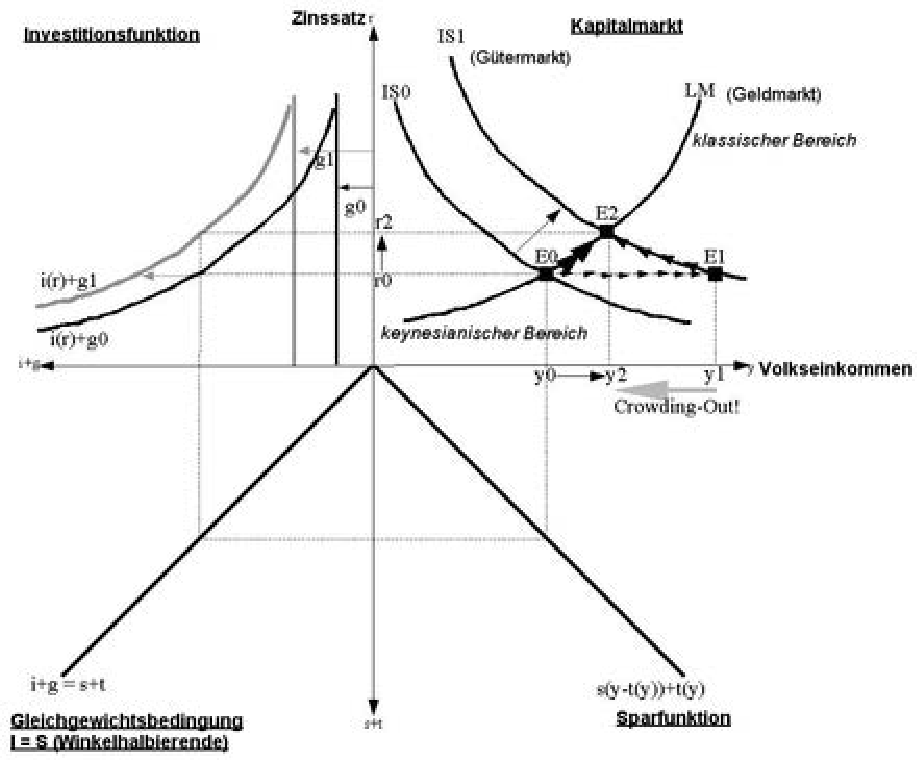
\includegraphics[width=0.75\textwidth]{Bilder/Keynes_IS_LM_Kreditfinanzierte_Steuersenkung.pdf}\\
\item Erh\"{o}hung der autonomen Investitionen
  \begin{align*}
    dI_{aut}&>0;\\
  \frac{dY}{dI_{aut}} &= \frac{1}{1-c +\frac{b l}{k}} >0\\
  \frac{di}{dI_{aut}} &= \frac{l}{k} \frac{dY}{dI_{aut}} >0
  \end{align*}
  \begin{align*}
    dI_{aut}&>0; dM_{aut}=dT_{aut}=dC_{aut}=dG_{aut}=dP=0, P=1\\
  dY &= \frac{1}{1-c -\frac{b L_Y}{L_i}} \left(\underbrace{dI_{aut}}_{>0}\right) >0\\
  di &= \frac{-L_Y}{L_i} dY >0
  \end{align*}
  Grafik v\"{o}llig analog zu Kreditfinanzierten Staatsausgabenerh\"{o}hungen.\\
  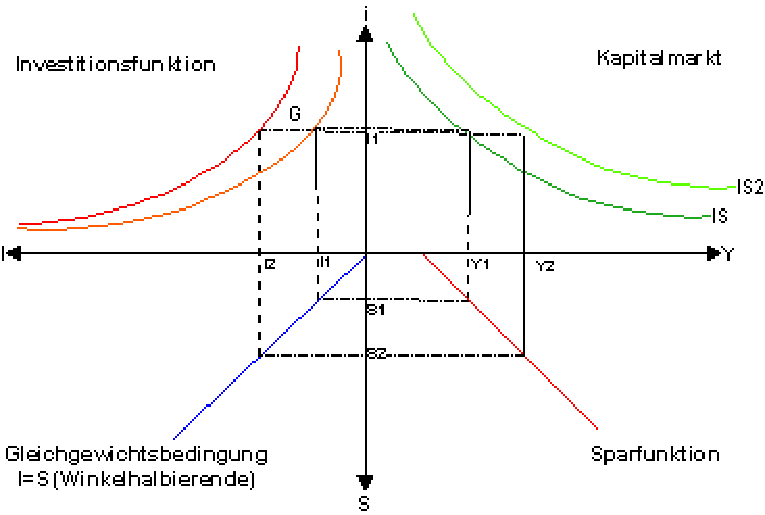
\includegraphics[width=0.75\textwidth]{Bilder/Keynes_IS_LM_Kreditfinanziert.pdf}\\
\item Erh\"{o}hung des Geldangebots: $dM>0$ (oder Senkung des Preisniveaus $dP<0$)
\begin{align*}
    \frac{dY}{dM} &= \frac{1}{1-c +\frac{b l}{k}} \left(\frac{b}{k} \frac{1}{P}\right) >0\\
    \frac{di}{dM} &= \frac{-1}{kP} dM+\frac{l}{k} dY \\
    di &= \frac{-1}{k}\left(1 - \frac{\frac{b l}{k}}{1-c+\frac{b l}{k}}\right) \frac{dM}{P} <0
\end{align*}
\begin{align*}
    dY &= \frac{1}{1-c -\frac{b L_Y}{L_i}} \left(- \frac{b}{L_i} \frac{1}{P}dM\right) >0\\
    di &= \frac{1}{L_iP} dM-\frac{L_Y}{L_i} dY = \frac{1}{L_i}\left(\frac{dM}{P}-L_Y \frac{1}{1-c -\frac{b L_Y}{L_i}} \left(- \frac{b}{L_i} \frac{1}{P}dM\right) \right)\\
    di &= \frac{1}{L_i}\left(1 + \frac{\frac{b L_Y}{L_i}}{1-c-\frac{b L_Y}{L_i}}\right) \frac{dM}{P} \frac{1}{L_i}\left(\frac{ 1-c-\frac{b L_Y}{L_i} + \frac{b L_Y}{L_i}}{1-c-\frac{b L_Y}{L_i}}\right) \frac{dM}{P}<0
\end{align*}
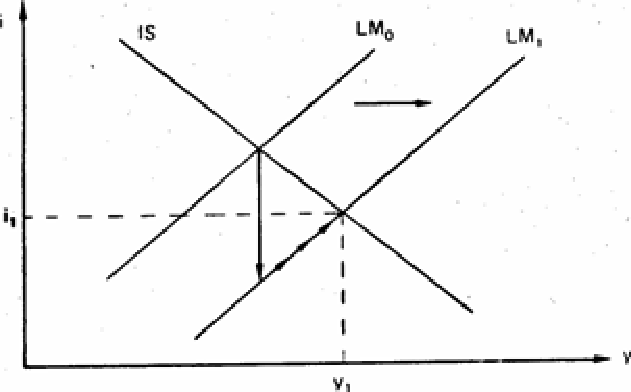
\includegraphics[width=0.75\textwidth]{Bilder/Keynes_IS_LM_Geldpolitik.pdf}\\
Zusammenfassend:\\
Korrelation zwischen Zins und Einkommen h\"{a}ngt von der Politikma{\ss}nahme ab:
\begin{itemize}
  \item Expansive Fiskalpolitik oder Investitionspolitik gibt positive Korrelation (Y steigt und Zins steigt)
  \item Expansive Geldpolitik gibt negative Korrelation (Y steigt und i sinkt)
\end{itemize}
\end{enumerate}
\end{enumerate}

\subsection{Sparquote im IS-LM Modell}
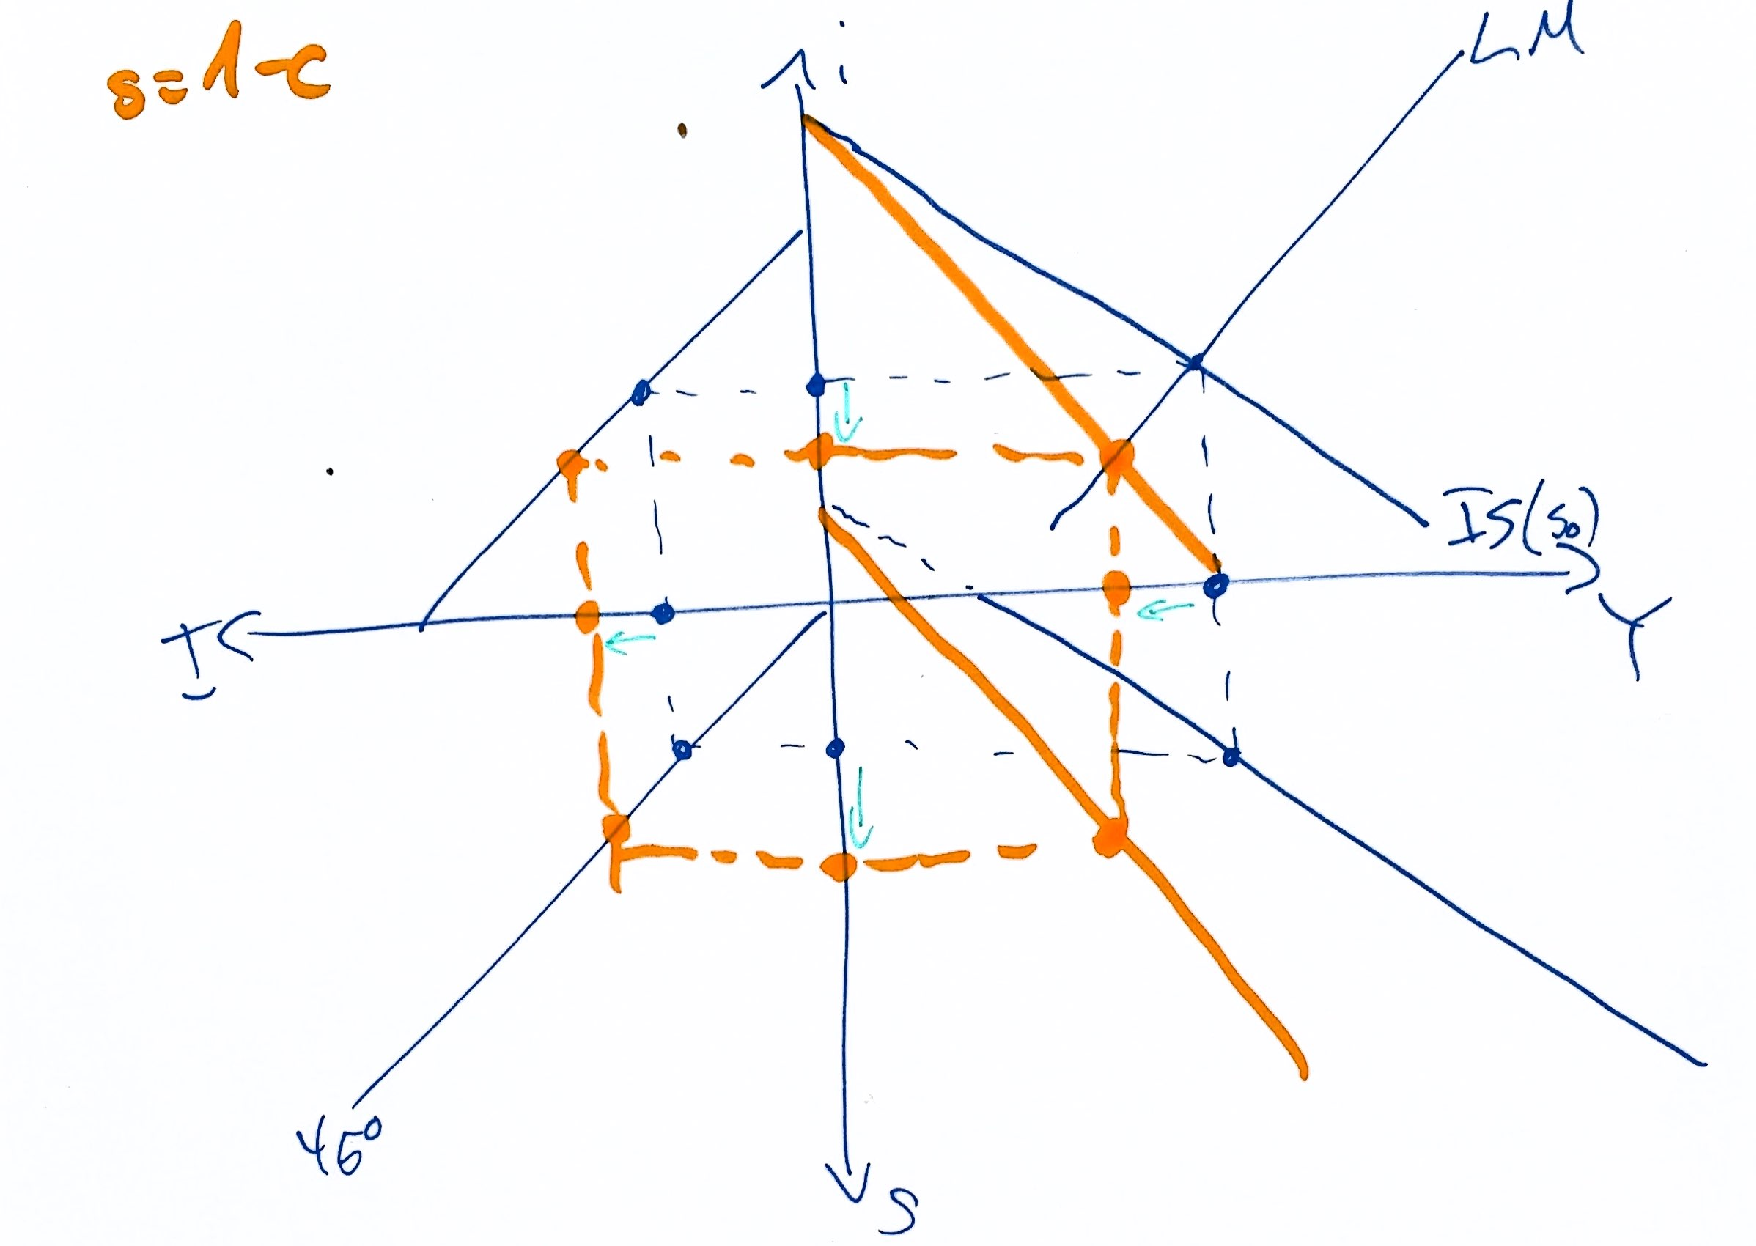
\includegraphics[width=.75\textwidth]{Bilder/Keynes_IS_LM_Sparquote.pdf}\\
Ergebnis: i sinkt, Y sinkt, S steigt, I steigt. Somit $L_s$ steigt und $L_T$ sinkt.


\subsection{Liquidit\"{a}tsfalle im IS-LM Modell}
\begin{enumerate}
  \item Falsch, bis sich Zins $R_0$ ann\"{a}hert
  \item Falsch, Einkommen steigt
  \item Wahr, $R_0$ ist minimalzins
  \item Wahr
  \item Wahr
  \item Falsch, IS-LM ist Konstruktion f\"{u}r Gleichgewichte!
\end{enumerate}

\subsection{Klassischer Verlauf der LM Kurve}
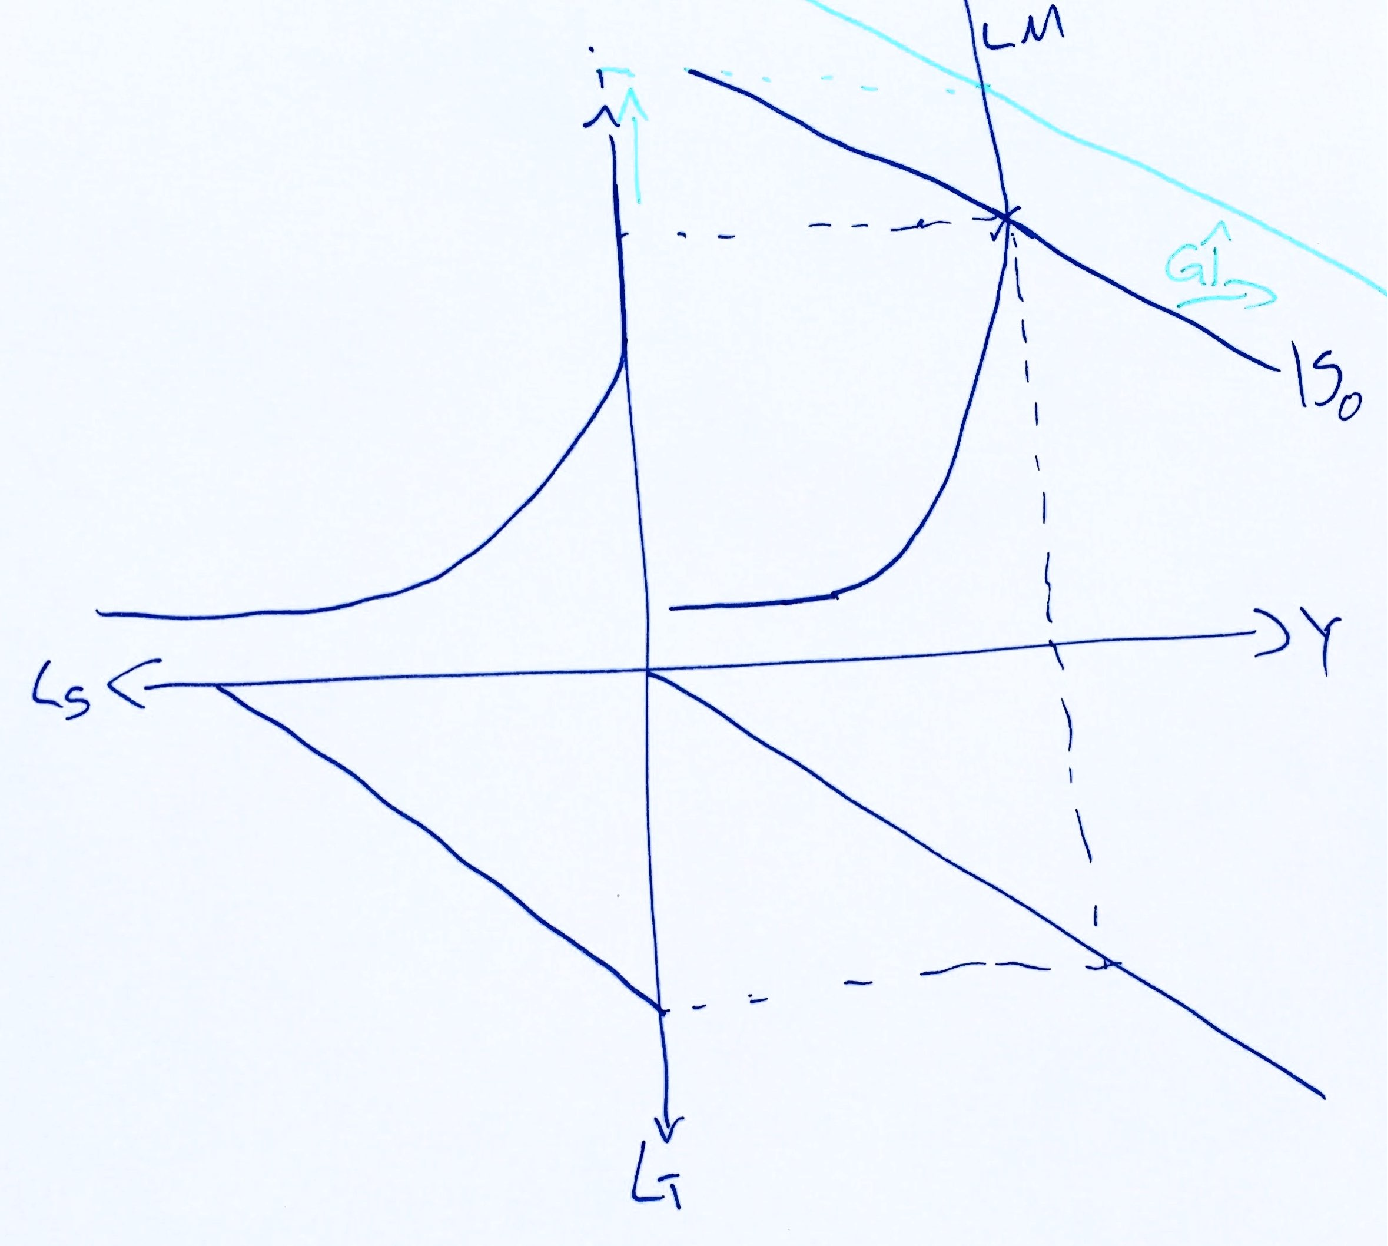
\includegraphics[width=.75\textwidth]{Bilder/Keynes_IS_LM_Klassische_LM_Kurve.pdf}\\
Ergebnis: i steigt, Y unver\"{a}ndert, $L_s$ unver\"{a}ndert, da Zinsunabh\"{a}ngig, $L_T$ unver\"{a}ndert. Da $i$ steigt: S und I sinken.


\subsection{Investitionsfalle im IS-LM Modell}
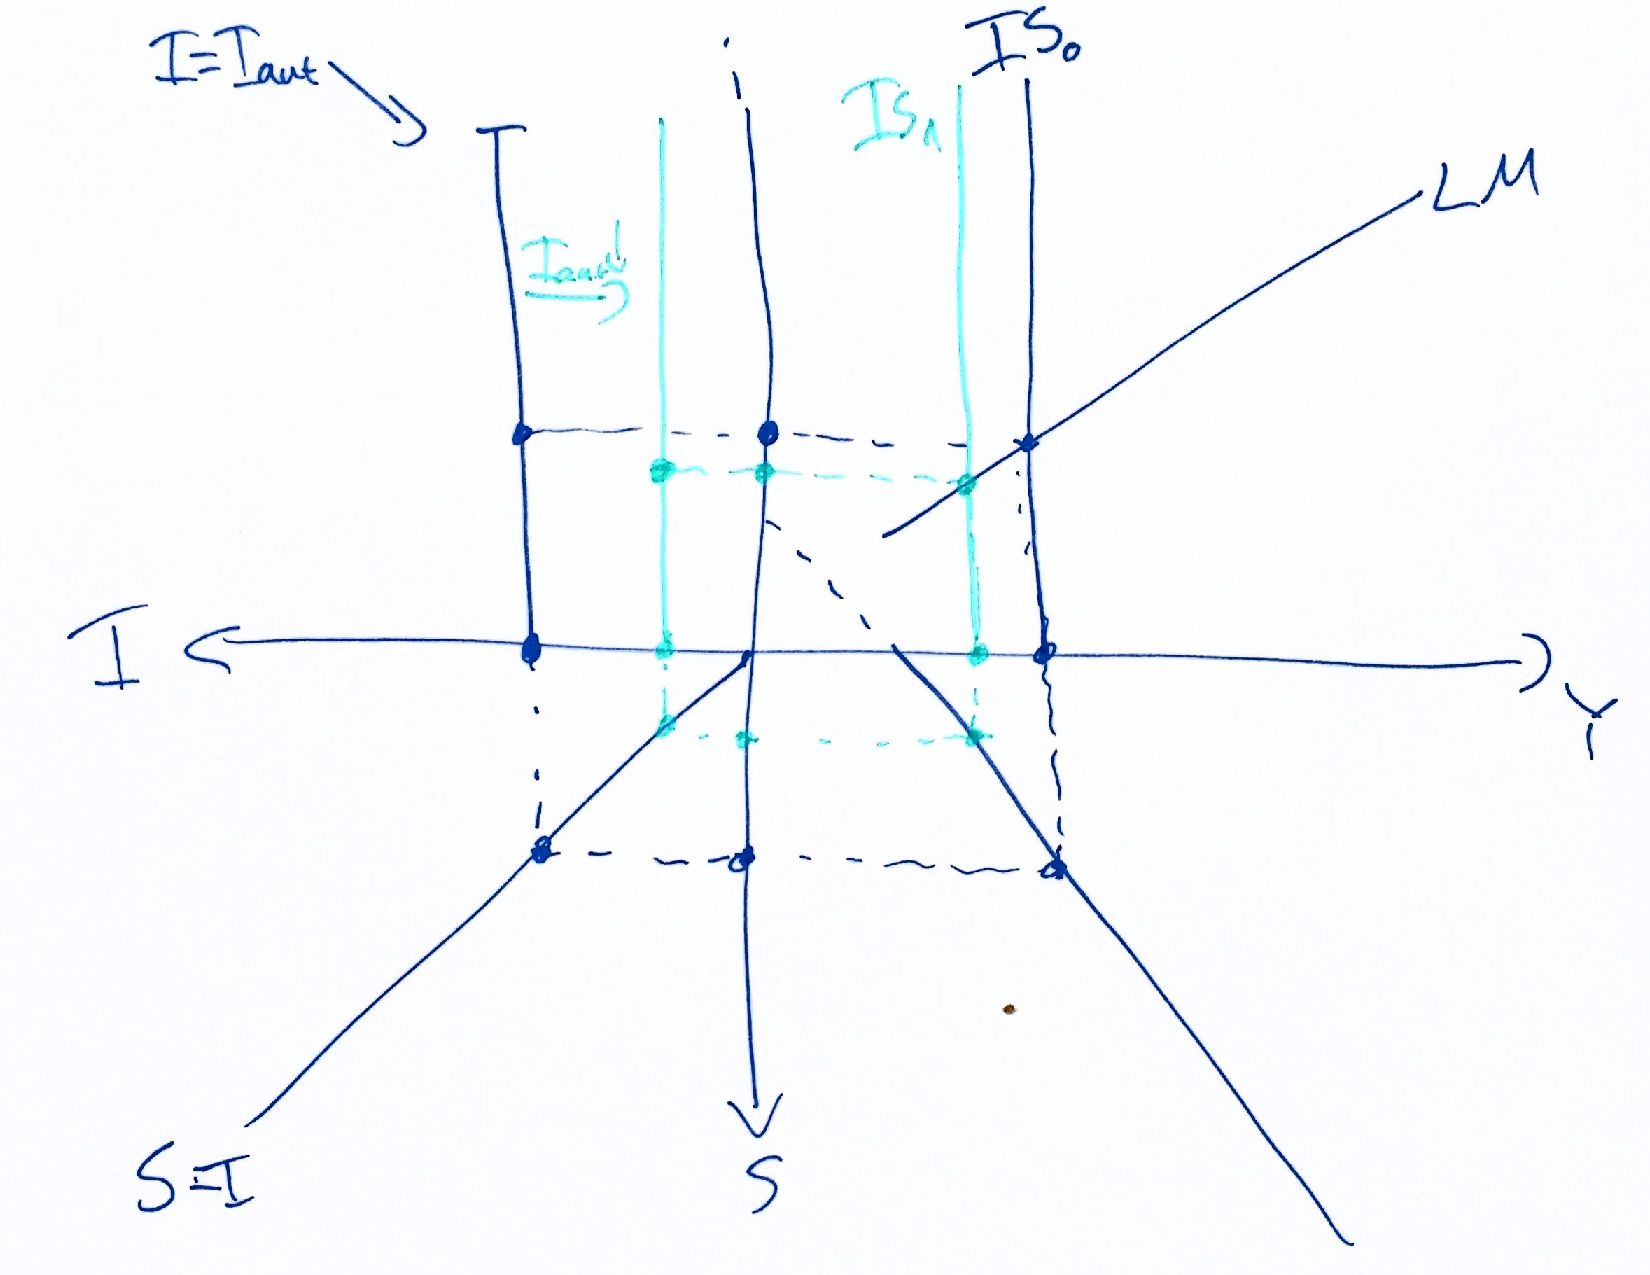
\includegraphics[width=.75\textwidth]{Bilder/Keynes_IS_LM_Investitionsfalle.pdf}\\
Ergebnis: i sinkt, Y sinkt, S sinkt, I sinkt. Somit $L_s$ steigt und $L_T$ sinkt.


\subsection{Rechenaufgabe}
\begin{enumerate}
  \item \begin{align*}
    Y^s=Y^d \Leftrightarrow Y = C + I + G = \frac{1}{5}Y + 60 \Leftrightarrow Y^* = 75
  \end{align*}
  \item \begin{align*}
    dY &= \frac{-c}{1-c(1-q)} dT_{aut} = \frac{-1/2}{4/5} dT_{aut} = -5\\
    dT^* &= dT_{aut} + \frac{3}{5}dY = 5
  \end{align*}
  \item \begin{align*}
    \text{IS: } Y &= \frac{1}{5}Y + 70 -40 i; C=\frac{1}{5}Y\\
    \text{LM: } \frac{M}{P} &= L \Leftrightarrow11.5 = \frac{1}{5}Y -30i = C-30i\\
    \text{IS: } \frac{4}{5} Y &= 70-40i\\
    C=\frac{1}{5}Y &= \frac{70}{4}-10i = 11.5 + 30i = \frac{46}{4}+30i \Leftrightarrow 6 = 40i\\
    \Rightarrow \frac{4}{5} Y &= 4 C = 70-6 = 64 \Rightarrow C^*=16
  \end{align*}
\end{enumerate}


\subsection{Verst\"{a}ndnisfragen Keynesianische Theorie}
\begin{enumerate}
  \item wahr, wir brauchen noch z.B. starre Nominall\"{o}hne
  \item falsch, jedes GG ist m\"{o}glich
  \item Falsch, Keynesianische GG Begriff beschreibt einen Zustand mit Beharrungsverm\"{o}gen
  \item Falsch, Absolute Einkommenshypothese
  \item Falsch, h\"{o}herer Konsum verbessert \"{u}ber Multiplikator die aggregierte Nachfrage
  \item Wahr!
  \begin{itemize}
  \item Minimalmodel: $d Y = \frac{1}{1-c}(d G_{aut} + d C_{aut})$
  \item Modell mit Steuern: $d Y = \underbrace{\frac{1}{1-c(1-q)}}_{Multiplikator}\underbrace{(d G_{aut} + d C_{aut} - c d T_{aut})}_\text{Summe autonomer Gr\"{o}{\ss}en}$
  \end{itemize}
  \item Falsch, Marktr\"{a}umung ist G\"{u}terangebot=G\"{u}ternachfrage
  \item Falsch! $I=S$ und $Y^d=C+I+G$ sind \"{a}quivalent!
  \item Falsch, da Pauschalsteuer in Konsumfunktion eingeht: \\$Y = \frac{1}{1-c(1-q)}(\dots+G_{aut}-c T_{aut}+\dots)$.
  \item Wahr, dies ist die Definition
  \item Wahr
\end{enumerate}

\section{Lundberg und Robertson-Lag}
\subsection{Verst\"{a}ndnisfragen}
\begin{enumerate}
  \item Lags
  \begin{itemize}
  \item Lundberg: Fokus auf Verz\"{o}gerung zwischen \"{A}nderung der Nachfrage und Antwort des Outputs, ungeplante Investitionen k\"{o}nnen auftreten
  \item Robertson: Fokus auf Verz\"{o}gerung im Konsum aufgrund einer Einkommens\"{a}nderung, ungeplante Ersparnis kann auftreten
  \end{itemize}
  \item \begin{enumerate}[a)]
      \item \begin{align*}
        Y = C+I+G = C_{aut} + cY + I_{aut}+ G_{aut} \\
        \Rightarrow Y^* = \frac{1}{1-c}(C_{aut}+I_{aut}+G_{aut})= \frac{1}{1-0.5}(50+50+100)=400
      \end{align*}
  \item Lundberg-Lag: Produktion richtet sich nach Gesamtnachfrage der Vorperiode, d.h.
  \begin{align*}
    Y_t &= Y_t^s = Y_{t-1}^d = C_{t-1} + I_{t-1}+G_{t-1}\\
    C_t &= C_{aut}+c Y_t\\
    S_t &= Y_t - C_t\\
    I_{ungepl,t} &= S_t - I_{t} - G_t \text{ wenn $G_t$ kreditfinanziert ist}
  \end{align*}
  Robertson-Lag: Konsum richtet sich nach Einkommen der Vorperiode
  \begin{align*}
    C_t &= C_{aut} + c Y_{t-1}\\
    Y_t &= C_t + I_t + G_t\\
    S_{gepl,t} &= Y_{t-1}-C_t\\
    S_t &= I_t + G_t \text{ wenn $G_t$ kreditfinanziert ist}\\
    S_{ungepl,t} &= S_t - S_{gepl,t} = I_t+G_t - S_{gepl,t}
  \end{align*}
  \item in $t+1:$ $G_{aut}=150$,
  Neues GG: $Y^* = \frac{1}{1-0.5}(50+50+150) = 500, C^* = 300$\\
  Lundberg-Lag\\
  \begin{tabular}{|c|c|c|c|c|}
    \hline
    % after \\: \hline or \cline{col1-col2} \cline{col3-col4} ...
      & $C_t=C_{aut}+c Y_t$ & $I_{aut}$ & $G_t$ & $Y_t =C_{t-1}+I_{t-1}+G_{t-1}$ \\\hline
    0 & 250 & 50 & 100 &  \\
    1 & 250 & 50 & 150 & 400 \\
    2 & 275 & 50 & 150 & 450 \\
    3 & 287,5& 50 & 150 & 475 \\
    $\vdots$ & $\vdots$ & $\vdots$ & $\vdots$ & $\vdots$ \\
    $\infty$ & 300 & 50 & 150 & 500 \\
    \hline
  \end{tabular}\\

  Robertson-Lag\\
    \begin{tabular}{|c|c|c|c|c|}
    \hline
    % after \\: \hline or \cline{col1-col2} \cline{col3-col4} ...
      & $C_t=C_{aut}+c Y_{t-1}$ & $I_{aut}$ & $G_t$ & $Y_t =C_{t}+I_{t}+G_{t}$ \\\hline
    0 & 250 & 50 & 100 & 400 \\
    1 & 250 & 50 & 150 & 450 \\
    2 & 275 & 50 & 150 & 475 \\
    3 & 287,5& 50 & 150 & 487,5 \\
    $\vdots$ & $\vdots$ & $\vdots$ & $\vdots$ & $\vdots$ \\
    $\infty$ & 300 & 50 & 150 & 500 \\
    \hline
  \end{tabular}
  \end{enumerate}

\end{enumerate}

\subsection{Rechenaufgabe Robertson Lag}
Neues GG: $Y^* = \frac{1}{1-0.75}(0+30+25) = 220, C^* = 0,75\cdot220=165$
\begin{center}
\begin{tabular}{|l|l|l|l|l|l|}
\hline
Periode        & 0   & 1                            & 2                                    & ... & $\infty$ \\ \hline
$Y_{t-1}$      & 140 & 140                          & 160                                  & ... & \textcolor{red}{$\frac{1}{1-0.75}(0+30+25) = 220$}         \\ \hline
$C_t$          & 105 & 105                          & \textcolor{red}{$0,75\cdot160 =120$} & ... & \textcolor{red}{$0,75\cdot220=165$}         \\ \hline
$I_{t}$        & 10  & 30                           & 30                                   & ... & 30       \\ \hline
$G_t$          & 25  & 25                           & 25                                   & ... & 25       \\ \hline
$Y_t$          & 140 & 160                          & \textcolor{red}{120+30+25=175}       & ... & \textcolor{red}{$\frac{1}{1-0.75}(0+30+25) = 220$}          \\ \hline
$S_{gepl,t}$   & 35  & \textcolor{red}{140-105=35}  & \textcolor{red}{160-120=40}          & ... & \textcolor{red}{220-165=55}         \\ \hline
$S_{ungepl,t}$ & 0   & \textcolor{red}{30+25-35=20} & \textcolor{red}{30+25-40=15}         & ... & 0        \\ \hline
\end{tabular}
\end{center}


\subsection{Rechenaufgabe Lundberg Lag}
Neues GG: $Y^* = \frac{1}{1-0.8}(0+30+10) = 200, C^* = 0,8\cdot200=160$
\begin{center}
\begin{tabular}{|l|l|l|l|l|l|}
\hline
Periode        & 0   & 1                              & 2   & ... & $\infty$ \\ \hline
$Y_{t}$        & 150 & 150                            & \textcolor{red}{120+30+10=160} & ... & \textcolor{red}{$\frac{1}{1-0.8}(0+30+10) = 200$}\\ \hline
$C_t$          & 120 & 120                            & \textcolor{red}{$0,8\cdot160=128$}   & ... & \textcolor{red}{$0,8\cdot200=160$}      \\ \hline
$I_{t}$        & 30  & 30                             & 30                             & ... & 30       \\ \hline
$G_t$          & 0   & 10                             & 10                             & ... & 10       \\ \hline
$S_t$          & 30  & \textcolor{red}{150-120=30}    & \textcolor{red}{160-128=32}    & ... & \textcolor{red}{200-160=40}       \\ \hline
$I_{ungepl,t}$ & 0   & \textcolor{red}{30-30-10=-10}  & \textcolor{red}{32-30-10=-8}   & ... & 0        \\ \hline
\end{tabular}
\end{center}

\section{Hick'sche Wachstumsmodell}
\subsection{Verst\"{a}ndnisfragen}
\begin{enumerate}[a)]
  \item Konjunktur-Modell im Keynesianischen Modell (Multiplikator), aber mit ver\"{a}nderter Investitionsgleichung.\\
  \begin{enumerate}[(1)]
  \item Gleichung: Konsumgleichung mit Robertson-Lag (Konsumverz\"{o}gerung h\"{a}ngt ab von EK der Vorperiode)\\
  \item Gleichung: Investitionen h\"{a}ngen ab von Ver\"{a}nderung im Output\\
  \Tree [.{Investitionen} [.{Bestandteil der Nachfrage} ] [.{Wachstum des Kapitalstocks} [{Investitionsentscheidung\\bzgl. des angestrebten Kapitalstocks} Angebot ] ]]\\
  Annahme: Es gibt effizienten Kapitalstock --> Investitionen werden \"{u}ber diesen optimalen Kapitalstock bestimmt (nicht \"{u}ber Zins)
  \begin{align*}
    I_t = K_{t} - K_{t-1} = I_{aut} + a(Y_{t-1}-Y_{t-2})
  \end{align*}
  Intuitiver Grund: Angestrebter Kapitalstock h\"{a}ngt von der angestrebten Produktion und damit von der erwarteten Nachfrage ab: $Y^d \uparrow \rightarrow K_p \uparrow \rightarrow I \uparrow$.\\
  Wichtig: Investitionen h\"{a}ngen nicht vom Niveau des EKs ab, sonder vom Wachstum des EKs!\\
  \item Gleichung: G\"{u}termarkt-GG
  \end{enumerate}
  \item Warum Akzelerator?\\
  EK steigt, angestrebter Kapitalstock steigt, Investitionen steigen, Nachfrage steigt, EK steigt, angestrebter Kapitalstock steigt $\Rightarrow$ EIMALIGER AKZELERATIONSPROZESS, da Wachstumsabh\"{a}ngig
  \item \begin{enumerate}[a)]
    \item Neues GG: $Y^*=\frac{1}{1-0.5}(100+50+50)=400$
    \item
        \begin{tabular}{|c|c|c|c|c|c|}
    \hline
    % after \\: \hline or \cline{col1-col2} \cline{col3-col4} ...
      & $C_t=C_{aut}+c Y_{t-1}$ & $I_{aut}$ & $I_{ind} = a(Y_{t-1} - Y_{t-2})$& $G_t$ & $Y_t =C_{t}+I_{t}+G_{t}$ \\\hline
    1 & 250 & 50 & 0 & 100 & 400 \\
    2 & 250 & 50 & 0 & 100 & 400 \\
    3 & 250 & 50 & 0 & 100 & 400 \\
    4 & 250 & 50 & 0 & 150 & 450 \\
    5 & 275 & 50 & 50 & 100 & 475 \\
    6 & 287,5& 50& 25 & 100 & 462,5 \\
    7 & 281,25& 50& -12.5 & 100 & 418.75 \\
    8 & 259,375& 50& -43.75 & 100 & <400 \\
    $\vdots$ & $\vdots$ & $\vdots$ & $\vdots$ & $\vdots$ &\vdots\\
    \hline
  \end{tabular}\\
Ek-Senkung in periode 6 aufgrund Akzelerator.
\item \begin{itemize}
  \item F\"{u}r $c < 2\sqrt{a}-a$ gibt es Schwingungen
  \item F\"{u}r $a \leq 1$ ist es stabil
\end{itemize}
  \end{enumerate}
\end{enumerate}

\subsection{Rechenaufgabe}
\begin{itemize}
\item
\begin{center}
\begin{tabular}{|l|l|l|l|l|l|}
\hline
Periode      & 0    & 1    & 2    & 3 \\ \hline
$C$          & 890  & 890  & 906  & 933,20          \\ \hline
$I_{ind}$    & 0    & 0    & \textcolor{red}{$0,9\cdot(1070-1050)=18$}     & 30,60       \\ \hline
$G$          & 20   & 40   & 40   & 40       \\ \hline
$Y$          & 1050 & 1070 & 1104 & \textcolor{red}{$933,20+30,60+40+\underbrace{140}_{I_{aut}}=1143,8$}          \\ \hline
\end{tabular}
\end{center}
\item Neues GG: $Y^* = \frac{1}{1-0.8}(50+140+40) = 1150$
\item Da $c < 2\sqrt{a}-a$ gibt es Schwingungen, aber da $a>1$ ist das System instabil und es existiert kein neues GG!
\end{itemize}


\section{Neoklassische Synthese}
\subsection{Aggregierte Nachfrage (AD-Modell)}
\begin{enumerate}
  \item Aggregierte Nachfragefunktion: Ordnet jedem p ein gleichgewichtiges Einkommen im IS-LM-Modell zu. Voraussetzung also: Angebot passt sich an Nachfrage an. Grob: Wie reagiert LM auf \"{A}nderungen von P?\\
  $P \uparrow \rightarrow L > \frac{M}{P} \rightarrow P_B \downarrow \rightarrow i \uparrow \rightarrow I \downarrow \rightarrow Y \downarrow$\\
  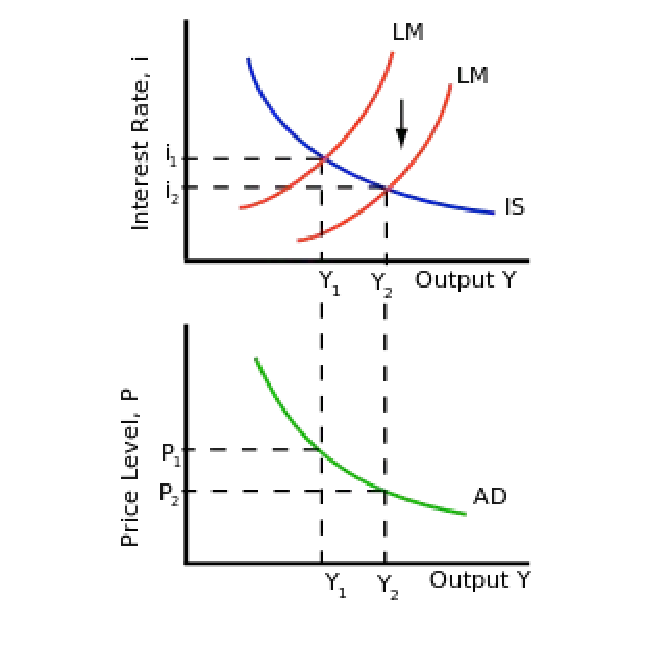
\includegraphics[width=0.5\textwidth]{Bilder/Neoklassische_Synthese_AD_Herleitung.pdf}\\
  Analytisch: LM nach i umformen und in IS einsetzen, ergibt:
  \begin{align*}
     Y &= \frac{1}{1-c -\frac{b L_Y}{L_i}} \left(C_{aut} - c T_{aut} + I_{aut} +G_{aut} - \frac{b}{L_i}\frac{M}{P}\right)\\
     dY &= \frac{1}{1-c -\frac{b L_Y}{L_i}} \left(dC_{aut} - c dT_{aut} + dI_{aut} +dG_{aut} - \frac{b}{L_i} \left(\frac{1}{P}dM-\frac{M}{P^2}dP\right)\right)\\
     \frac{dY}{dP} &= \frac{1}{1-c -\frac{b L_Y}{L_i}} \left(\frac{b}{L_i}\frac{M}{P^2}\right) <0
  \end{align*}
  Anstieg des Preisniveaus f\"{u}hrt zu Verknappung des realen Geldangebots. \"{U}berschussnachfrage nach liquiden Mitteln: HH wollen Wertpapiere ver\"{a}{\ss}ern, $P_B$ sinkt, Zins steigt, Investitionen werden zur\"{u}ckgedr\"{a}ngt und somit gesamtwirtschaftliche Nachfrage und Einkommen gesenkt.\\
  AD ist GG-Kurve und keine mikro\"{o}konomische Verhaltensbeziehung!\\
  Zinssatz\"{a}nderung:\\
  Entspricht der Frage nach dem Einfluss des Zinses auf das Einkommen im IS-LM-Modell
  \begin{itemize}
    \item Zins ist aber endogen!
    \item Jedem Punkt auf der AD-Kurve entspricht ein GG-Zins
    \item Einfluss also nicht feststellbar!
  \end{itemize}

  \item Lage der AD-Kurve:
  \begin{enumerate}
    \item $dG >0$ oder $dT<0$\\
      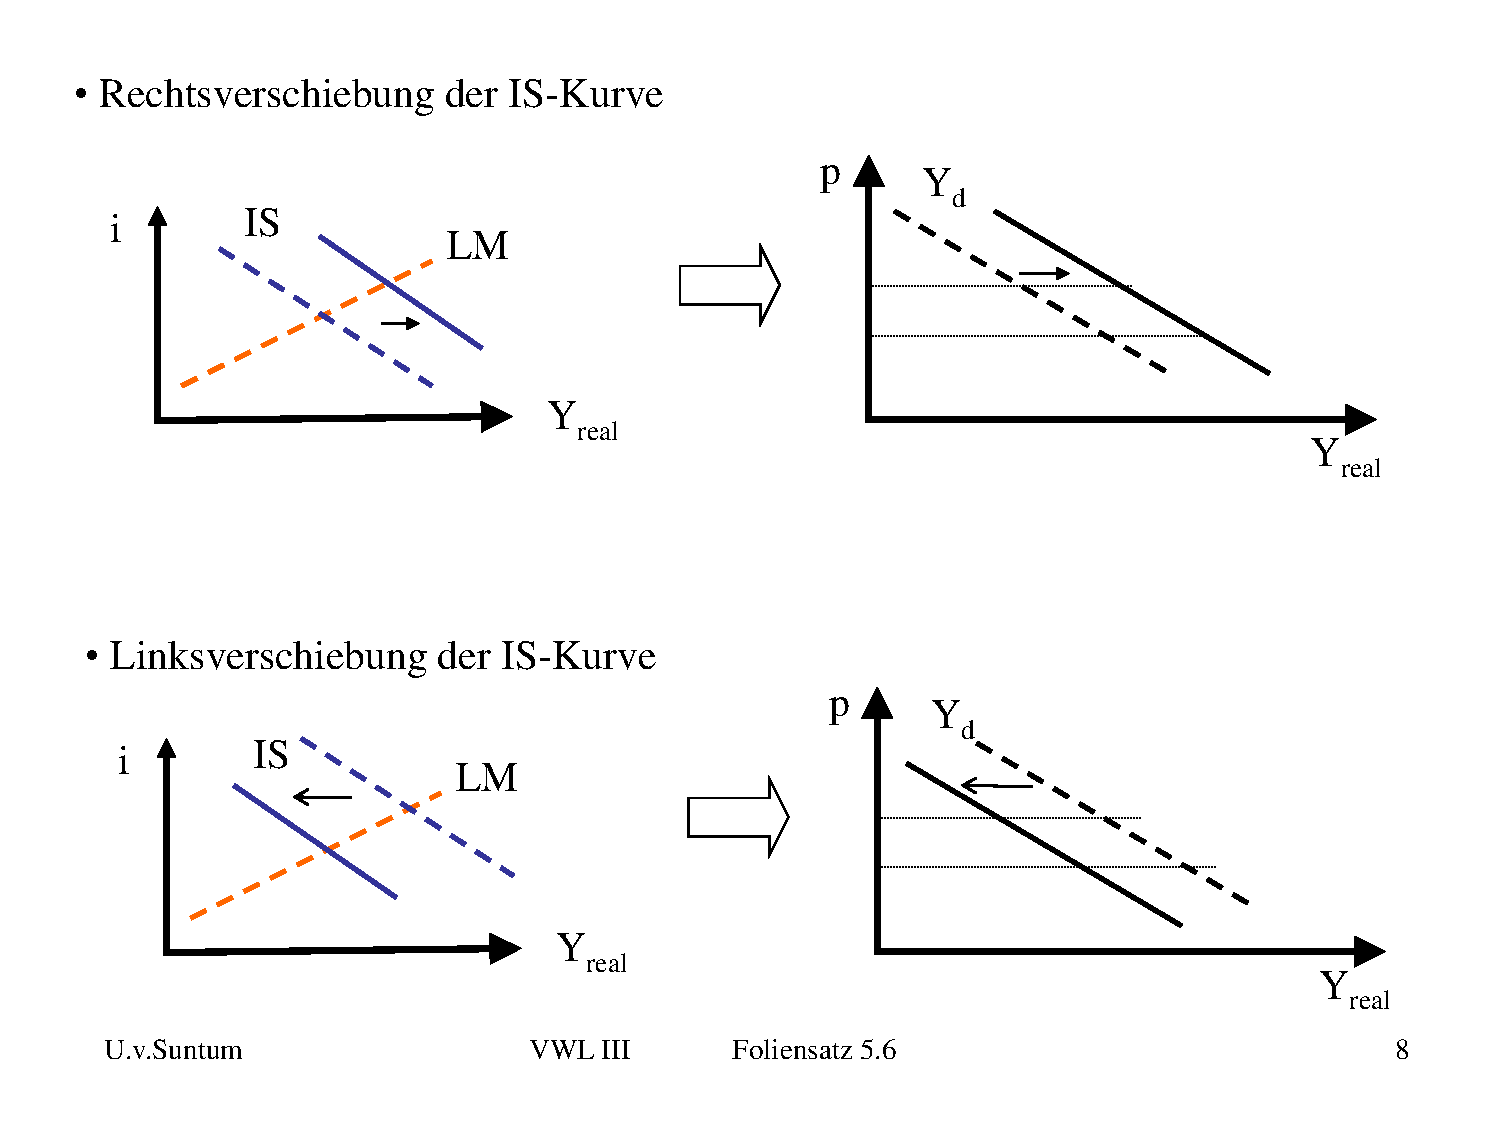
\includegraphics[width=0.8\textwidth]{Bilder/Neoklassische_Synthese_AD_Lage1.pdf}\\
    \item $dM >0$\\
        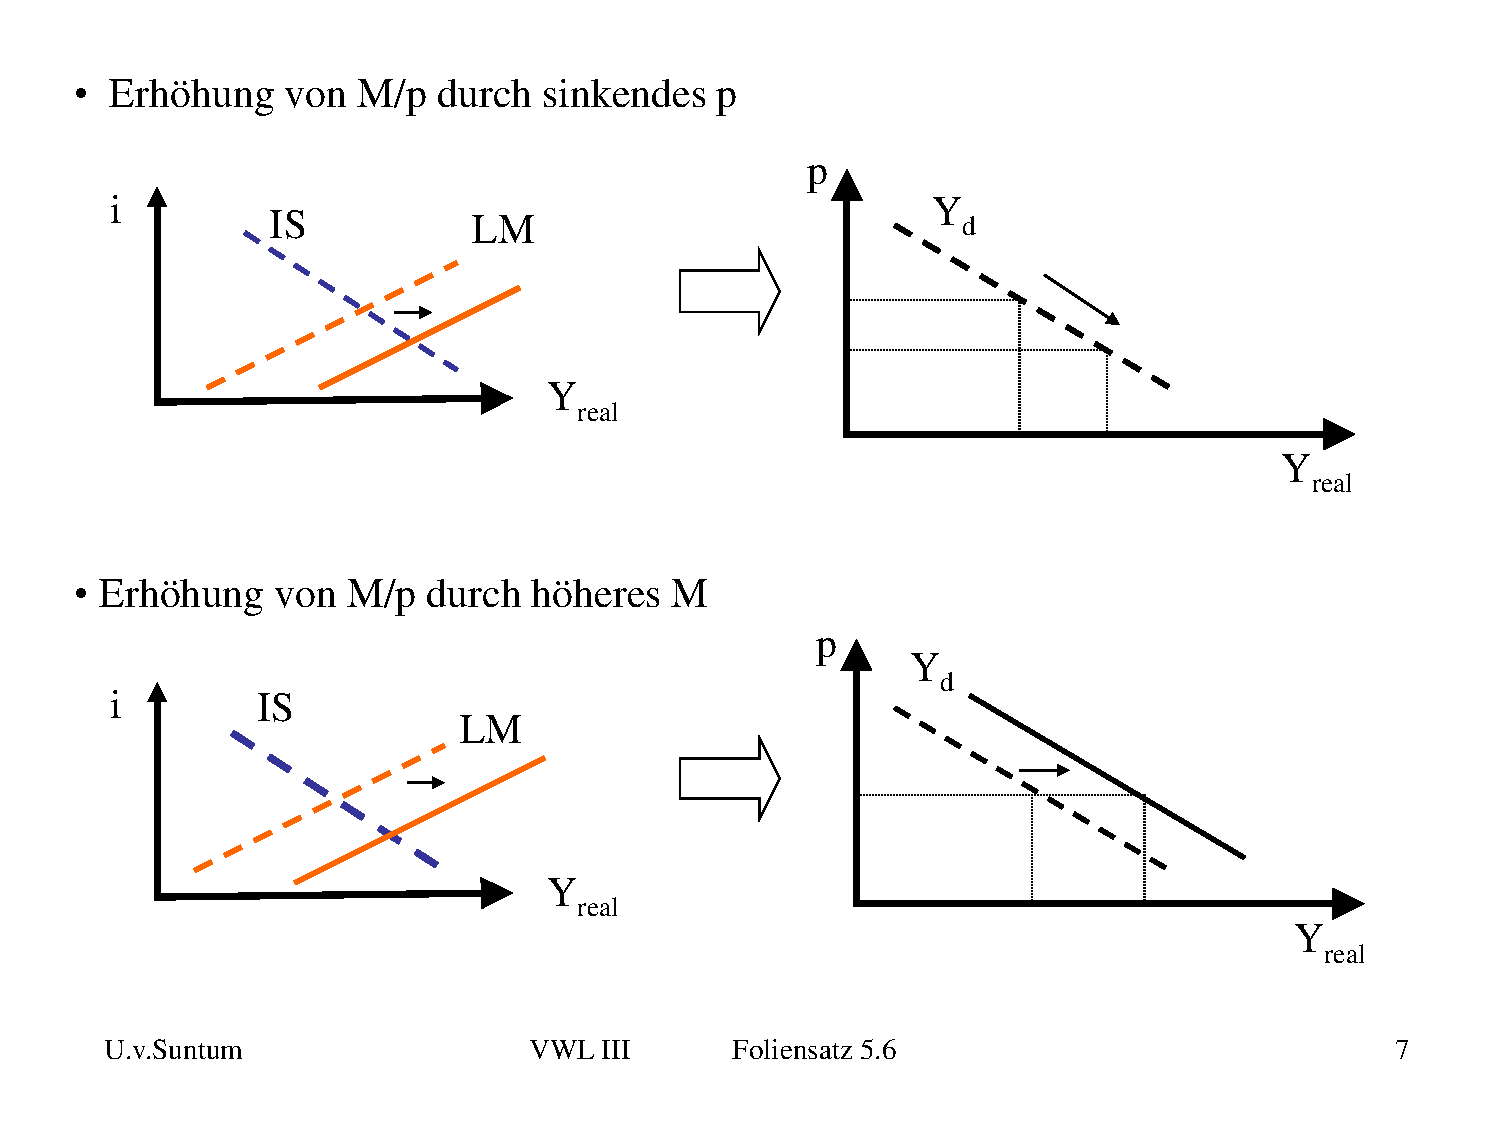
\includegraphics[width=0.8\textwidth]{Bilder/Neoklassische_Synthese_AD_Lage2.pdf}\\
  \end{enumerate}
  $AD: Y=Y^{AD}(\underbrace{\overset{+}{M},\overset{+}{G},\overset{-}{T}}_\text{Verschiebungen Kurve},\underbrace{\overset{-}{P}}_\text{Auf Kurve})$
\end{enumerate}


\subsection{Das allgemeine Keynesianische Modell bei festen Nominall\"{o}hnen}
\begin{enumerate}[(a)]
  \item Die Neoklassischen Synthese hat drei Punkte des Keynesianischen Nachfragesektors \"{u}bernommen:
  \begin{itemize}
    \item Abh\"{a}ngigkeit der Ersparnis/Konsum vom Einkommen
    \item Nicht-Neutralit\"{a}t des Geldes: H\"{o}he der Zinsen beeinflusst die mit der Ersparnis identische Investition beeinflusst und \"{u}ber die ver\"{a}nderte Investition, verst\"{a}rkt durch den Multiplikator, das Gesamteinkommen der \"{O}konomie
    \item Nominallohn kurzfristig fix, Preise sich nur langsam ver\"{a}ndernd
  \end{itemize}
  Aus der Neoklassik wird der Angebotssektor \"{u}bernommen:
  \begin{itemize}
    \item neoklassische Produktionsfunktion
    \item neoklassischer Arbeitsmarkt (Nachfrage und Angebot auf dem Arbeitsmarkt abh\"{a}ngig vom Reallohn)
  \end{itemize}
    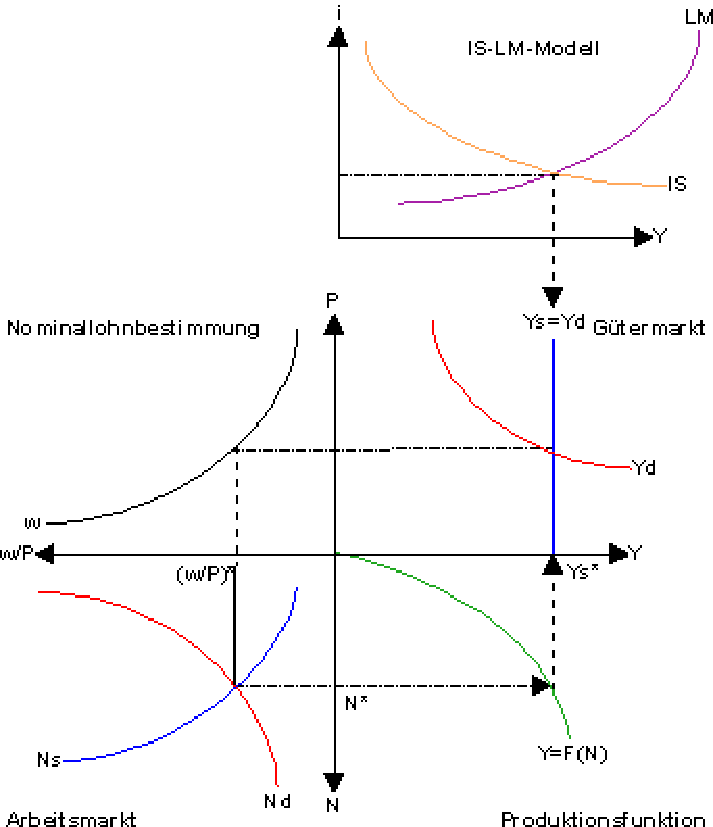
\includegraphics[width=0.5\textwidth]{Bilder/Neoklassische_Synthese_Normal.pdf}\\
\textbf{Der Keynes-Effekt:}\\
    Durch ein sinkendes Preisniveau ist das reale Geldangebot gr\"{o}{\ss}er als die Geldnachfrage (Transaktions- und Spekulationskasse). Haushalte und Unternehmen versuchen durch eine h\"{o}here Nachfrage am Wertpapiermarkt die \"{u}berh\"{o}hte Geldhaltung wieder abzubauen. Dabei kommt es mit der h\"{o}heren Nachfrage zu einem Anstieg der Wertpapierkurse und daraus resultierend zu sinkenden Zinsen. Bei sinkenden Zinsen steigen Investition, G\"{u}ternachfrage und Besch\"{a}ftigung gem\"{a}{\ss} dem Multiplikatorprozess. Keyens-Effekt wirkt jedoch nicht in der Investitions-oder Liquidit\"{a}tsfalle.

\item Gleichgewicht bei Unterbesch\"{a}ftigung\\
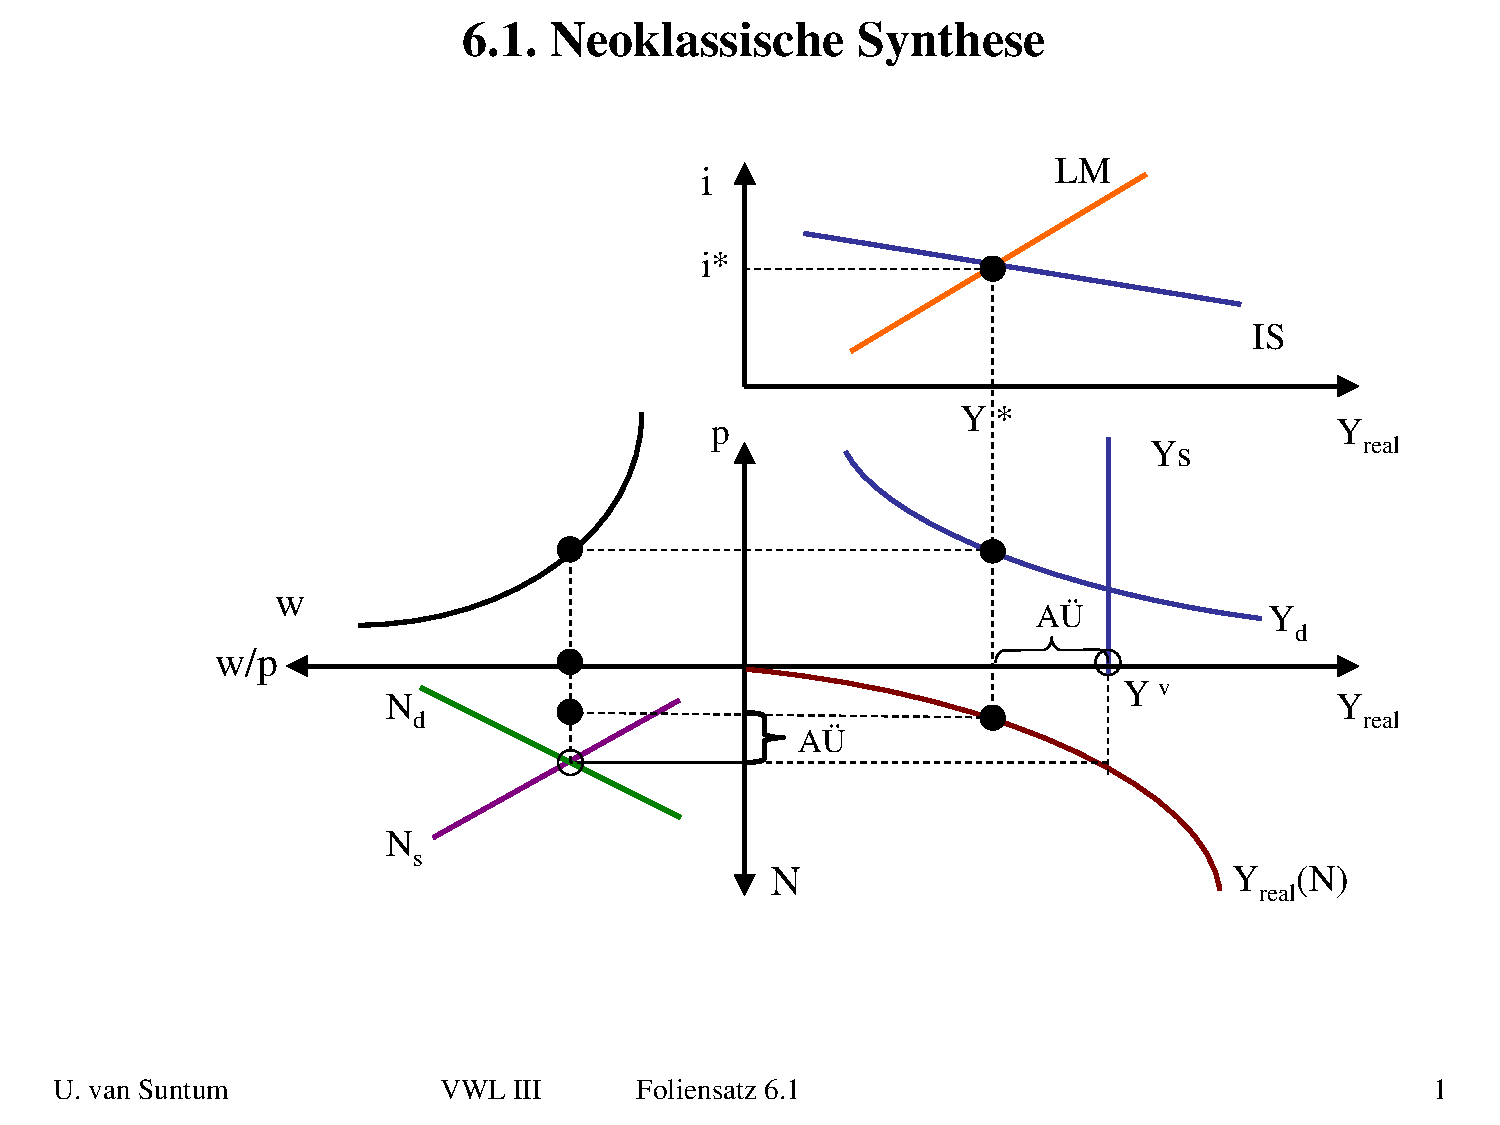
\includegraphics[width=\textwidth]{Bilder/Neoklassische_Synthese_Unterbeschaftigung.pdf}\\
\begin{itemize}
  \item Gleichgewicht auf Kapital-und Geldmarkt (IS/LM)
  \item Angebots\"{u}berschuss (A\"{U}) auf Arbeits-und G\"{u}termarkt
  \item Reallohnsenkung weder n\"{o}tig noch wirksam
  \item Unternehmen sind auf dem G\"{u}termarkt rationiert => Arbeitsnachfrage gilt hier nicht
  \item Arbeitnehmer sind auf dem Arbeitsmarkt rationiert
\end{itemize}
\item Denkbare Auswege:
\begin{itemize}
\item sinkende Preise und Nominall\"{o}hne (Bewegung auf AD nach rechts) --> Keynes-Effekt!
\item expansive Geld-oder Fiskalpolitik (Verschiebung von AD nach rechts)
\end{itemize}

\item
\begin{enumerate}[(i)]
  \item Investitionsfalle\\ 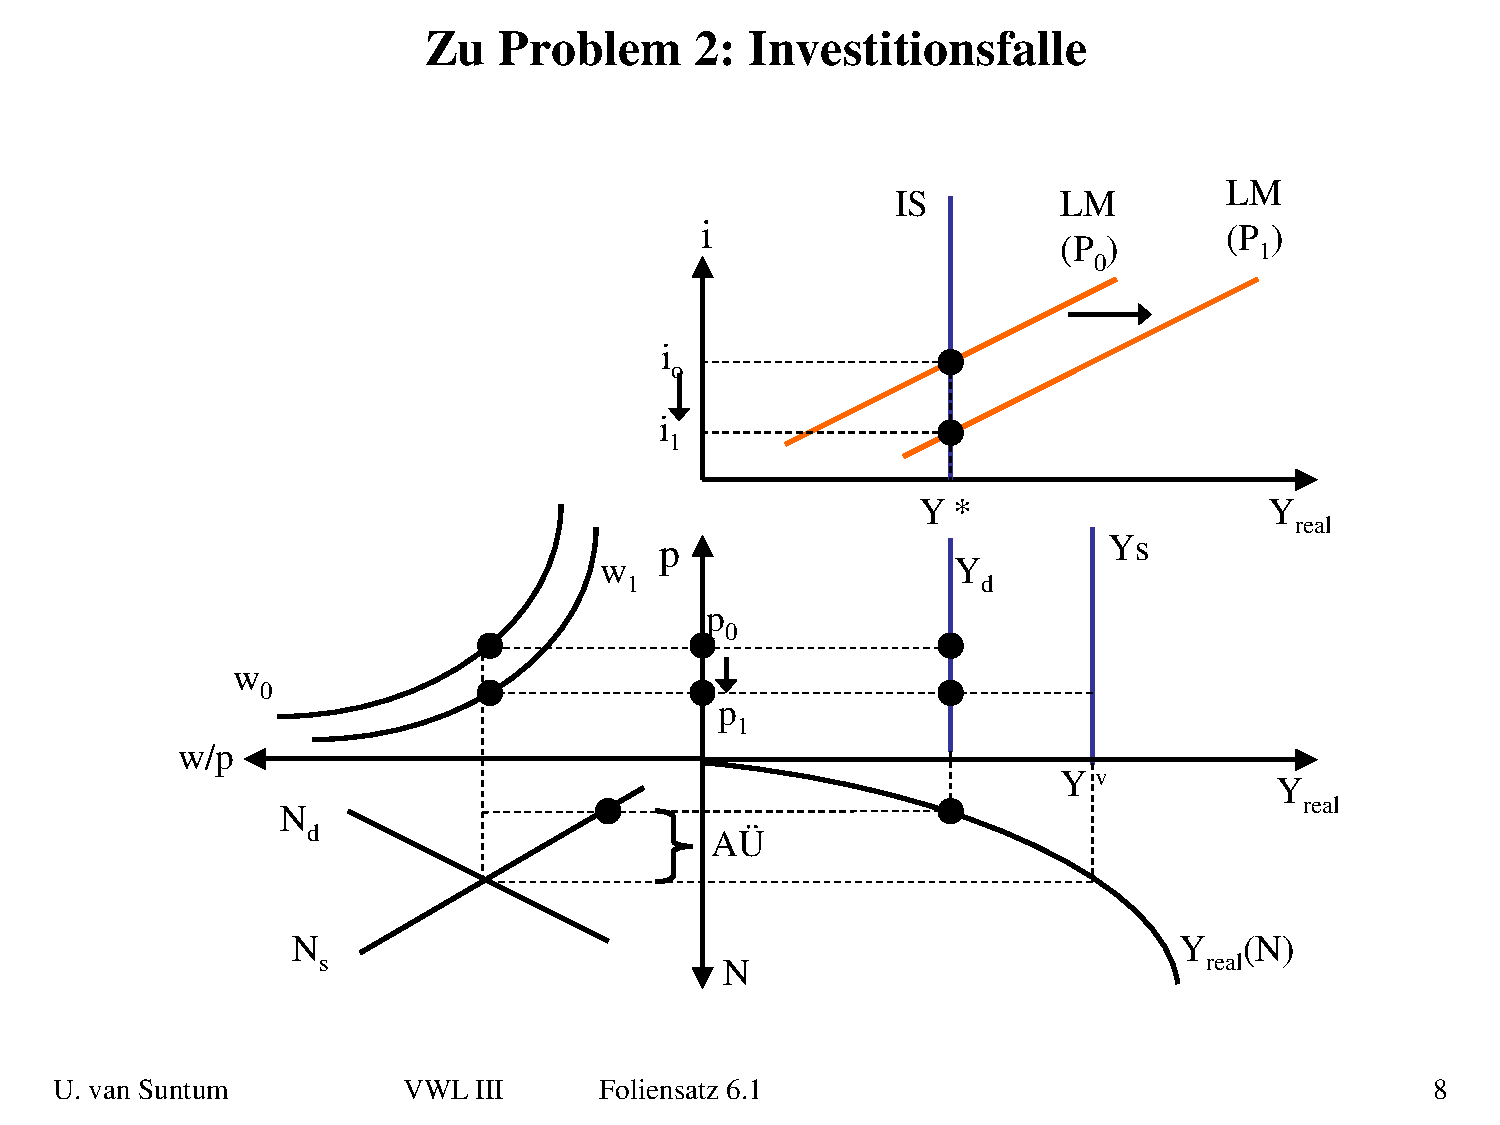
\includegraphics[width=\textwidth]{Bilder/Neoklassische_Synthese_Invest.pdf}\\
      Ausweg: Fiskalpolitik
  \item Liquidit\"{a}tsfalle \\ 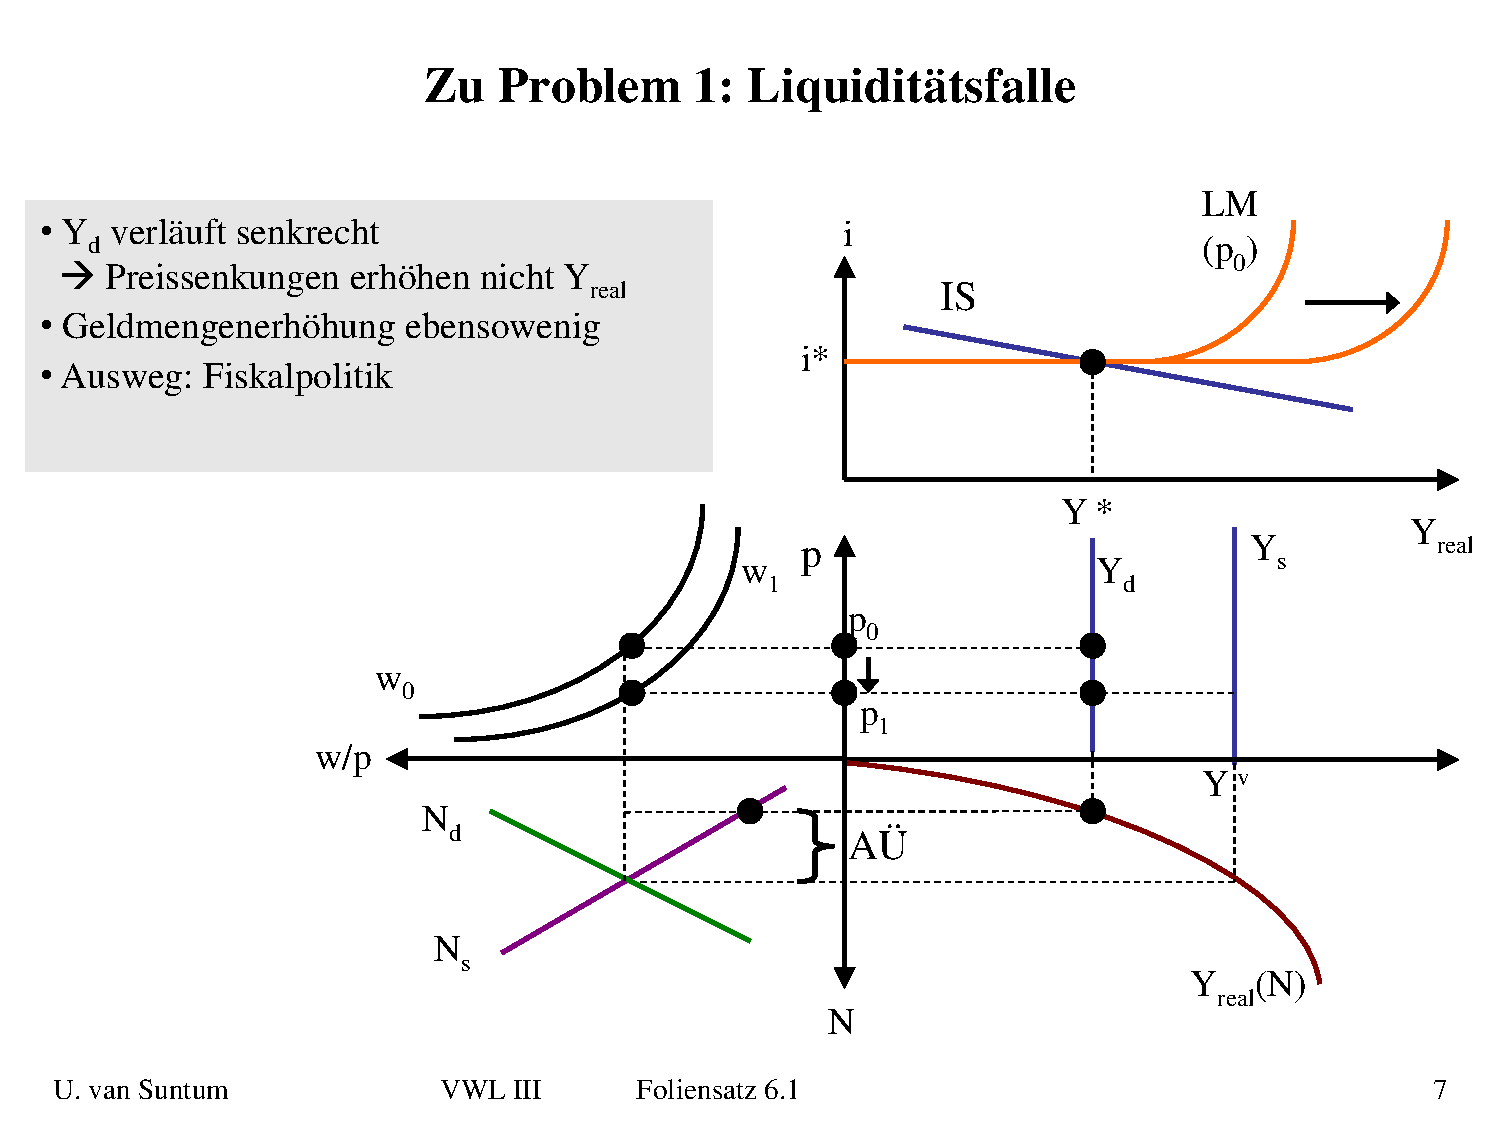
\includegraphics[width=\textwidth]{Bilder/Neoklassische_Synthese_Liquid.pdf}\\
Auswege Fiskalpolitik

\item Starre Nominall\"{o}hne\\ 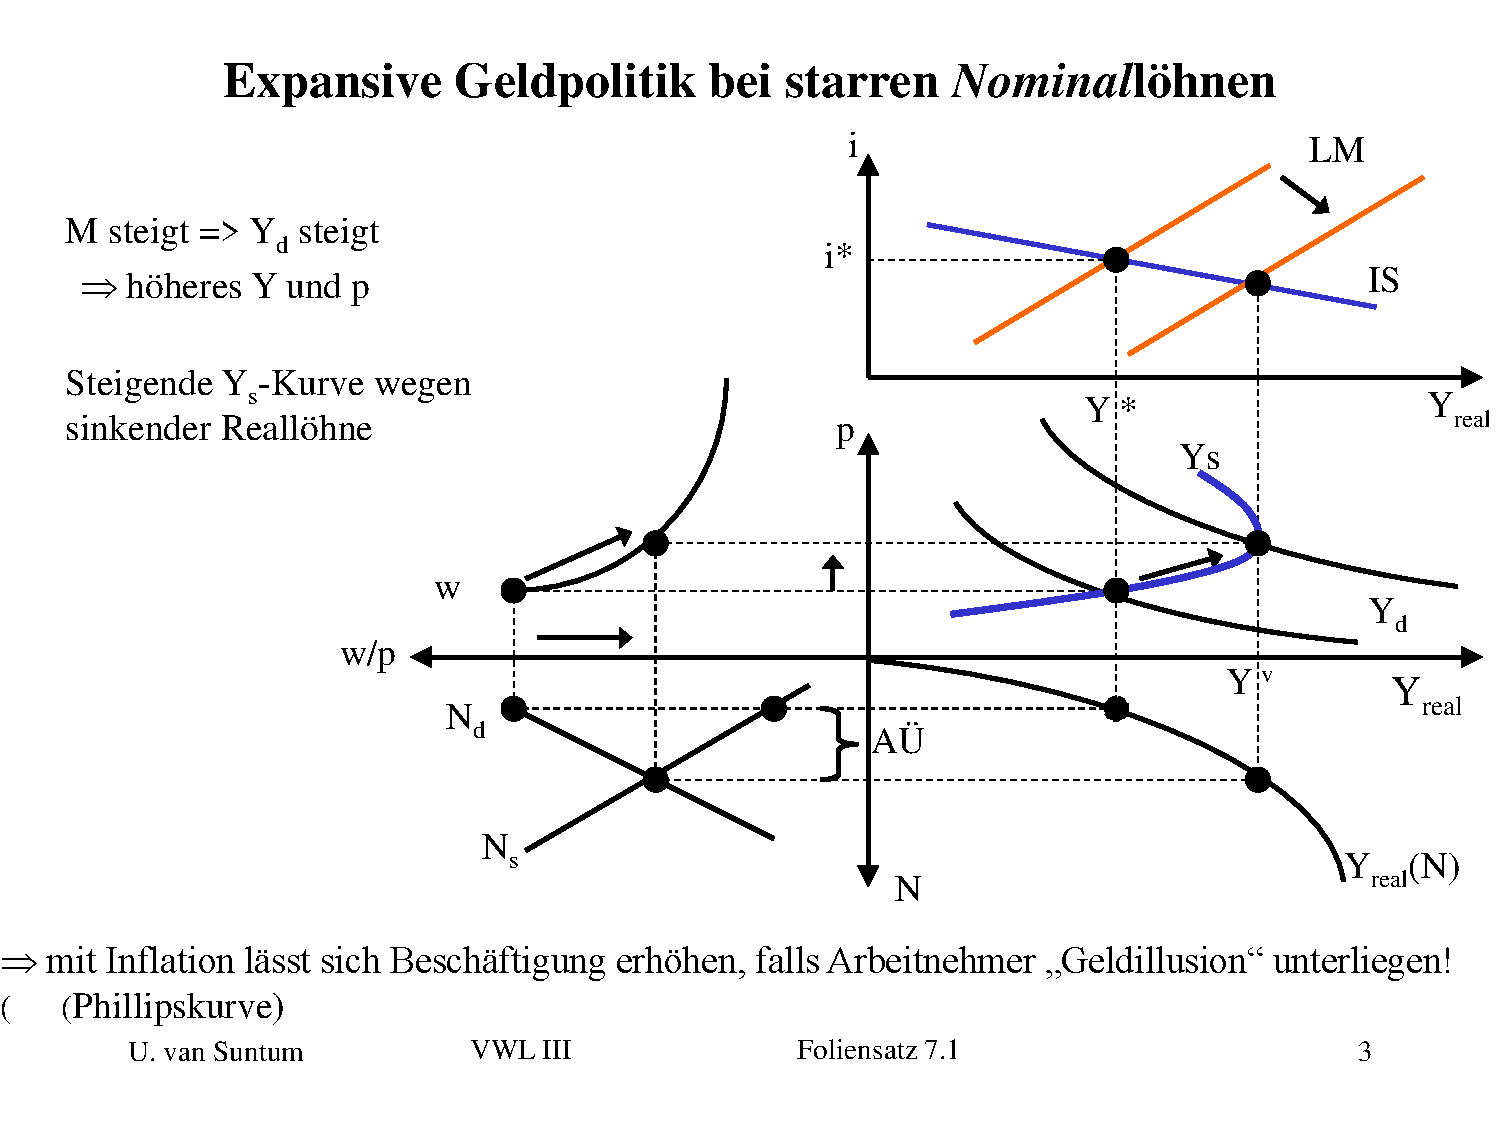
\includegraphics[width=\textwidth]{Bilder/Neoklassische_Synthese_Fix_Lohn_Geld.pdf}\\
    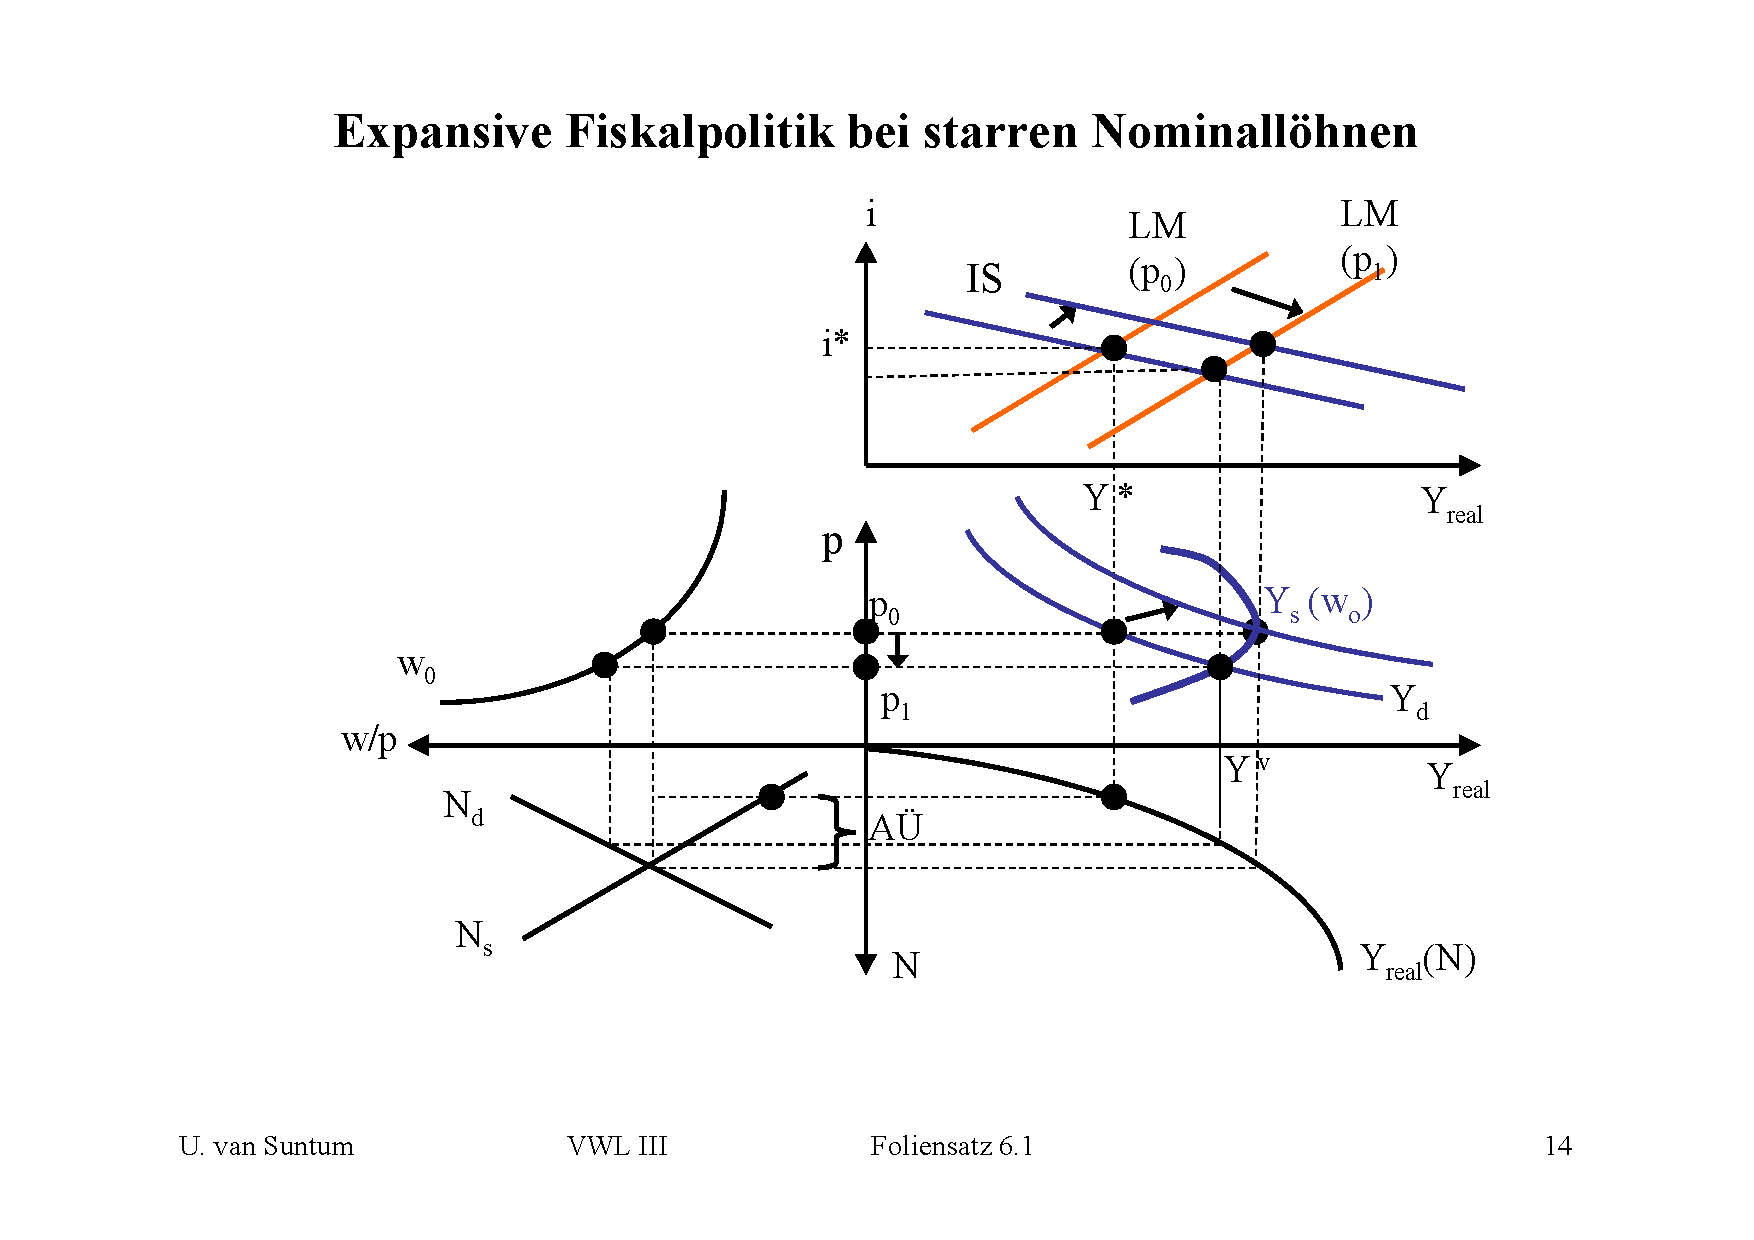
\includegraphics[width=\textwidth]{Bilder/Neoklassische_Synthese_Fix_Lohn_Fiskal.pdf}\\
Bei starren Nominall\"{o}hnen ist die Geldpolitik in der Lage, durch Inflation, das neoklassische Gleichgewicht zu erreichen. Fiskalpolitik auch denkbar.
\end{enumerate}
\end{enumerate}

\subsection{Demografische Entwicklung in der neoklassischen Synthese}

\subsection{Wirtschaftspolitische Ma{\ss}nahmen in der neoklassischen Synthese}
\end{document}
\section{Geldtheorie}
\subsection{Rechenaufgabe}
\begin{itemize}
  \item Geldmenge = Cash + Einlagen ($M=C+E \Leftrightarrow E=M-C$)
  \item Bargeldquote = Cash/Geldmenge ($c=C/M \Leftrightarrow C=cM$)
  \item Mindestreservesatz = Reserven/Einlagen ($r=RE/E \Leftrightarrow RE=rE=r(M-C)=r(M-cM)=r(1-c)M$)
  \item Geldbasis(ZB-Geld) = Cash + Reserven ($B=C+RE=cM + r(1-c)M \Leftrightarrow M=\frac{1}{c+r(1-c)}(C+RE)=mB$)
  \item Hier: m = 5.78
\end{itemize}




%%%%%%%%%%% AUSSORTIERT%%%%%%%%%%%%%%

\subsection{Lohnquote}
\begin{itemize}
    \item Unbereinigte Lohnquote: $Unb.LQ = \frac{ArbeitnehmerEinkommen}{Volkseinkommen}$
    \item $ArbeitnehmerEinkommen= \underbrace{Bruttoloehne}_{Nettoloehne+ANBeitr\"{a}ge} + AGBeitraege \\
    = (900+200)+300=1400$
    \item Volkseinkommen: $VE=\underbrace{BNE-Ab}_{NNE}-ind.Steuern+Unt.Subvent=2000-300-200+200=1700$
    \item $Unb.LQ=\frac{1400}{1700}=0.82$
    \begin{enumerate}[(a)]
      \item Anteil Selbst\"{a}ndiger $\uparrow$, ceteribus paribus ANEK $\downarrow$, LQ $\downarrow$
      \item Kein Effekt, da Arbeitnehmerbeitr\"{a}ge nur Aufteilung von Bruttol\"{o}hnen auf Arbeitnehmer und Sozialversicherung betreffen
      \item Kein Effekt, Konsum spielt auf der Verwendungsseite eine Rolle, nicht auf der Verteilungsseite!
    \end{enumerate}
\end{itemize}


\subsection{Lorenzkurve + Gini-Koeffizient}
\begin{center}
  \begin{tabular}{|c|c|c|c|c|}
     \hline
     % after \\: \hline or \cline{col1-col2} \cline{col3-col4} ...
     Person $i$ & EK $x_i$ & $\sum_{j=1}^i x_j$ & $u_i=\frac{i}{n}$ & $v_i=\frac{\sum_{j=1}^{i} x_j}{\sum_{j=1}^n x_j}$ \\\hline
     1 & 1 & 1 & $\frac{1}{10}$ & $\frac{1}{20}$ \\
     2 & 1 & 2 & $\frac{2}{10}$ & $\frac{2}{20}$ \\
     3 & 1 & 3 & $\frac{3}{10}$ & $\frac{3}{20}$ \\
     4 & 1 & 4 & $\frac{4}{10}$ & $\frac{4}{20}$ \\
     5 & 1 & 5 & $\frac{5}{10}$ & $\frac{5}{20}$ \\
     6 & 3 & 8 & $\frac{6}{10}$ & $\frac{8}{20}$ \\
     7 & 3 & 11 & $\frac{7}{10}$ & $\frac{11}{20}$ \\
     8 & 3 & 14& $\frac{8}{10}$ & $\frac{14}{20}$ \\
     9 & 3 & 17 & $\frac{9}{10}$ & $\frac{17}{20}$ \\
    (n=) 10 & 3 & 20 & $\frac{10}{10}$ & $\frac{20}{20}$\\\hline
     $\sum$ & 20
   \end{tabular}
  % Requires \usepackage{graphicx}
  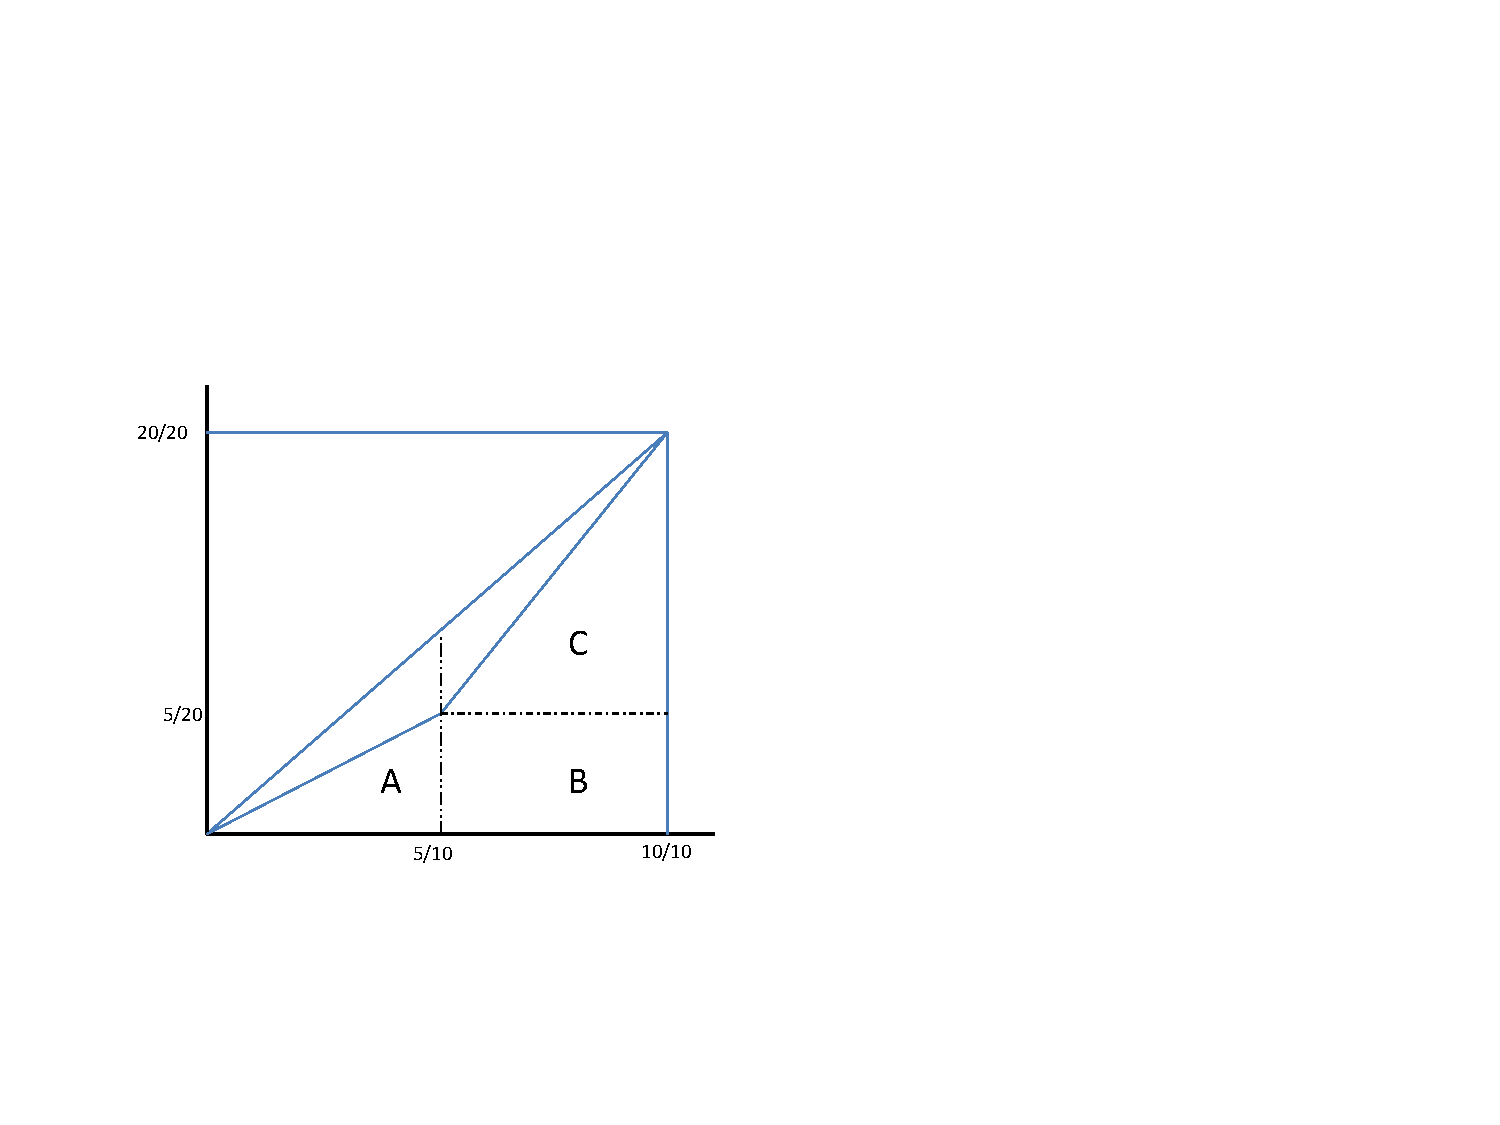
\includegraphics[width=.5\textwidth]{Bilder/lorenz.pdf}
\end{center}
Gini Koeffizient: $G = \frac{\text{Fl\"{a}che zwischen 45 Grad Diagonalen und Lorenzlinie}}{\text{Fl\"{a}che der Diagonalen}}$:
\begin{align*}
  G &= \frac{\overbrace{\frac{1}{2}\cdot1\cdot1}^\text{Fl\"{a}che Diagonale} - (\overbrace{\frac{1}{2} \cdot \frac{5}{10} \cdot \frac{5}{20}}^{A} +\overbrace{\frac{5}{10}\cdot\frac{5}{20} }^{B}+ \overbrace{\frac{1}{2} \cdot \frac{5}{10} \cdot \frac{15}{20}}^{C}  )}{\underbrace{\frac{1}{2}\cdot1\cdot1}_{\text{Fl\"{a}che Diagonale}}}\\
  &= \frac{\frac{1}{2} - (\frac{1}{16}+\frac{1}{8}+\frac{3}{16})}{\frac{1}{2}} = \frac{1}{4}
\end{align*}
\item
\textbf{Sparparadox:}
\begin{align*}
  S = S^{Pr}+S^{St} = I = \bar{I}\text{ mit } \bar{I} \text{ exogen}
\end{align*}
$S=(Y-T-C) + (T-G) = \bar{I}.$  Da $\bar{I}$ konstant ist, gilt dass, falls die Regierung spart, d.h. $S^{St}\uparrow$, muss $S^{Pr}$ im gleichen Ma{\ss}e sinken, da die Gesamtersparnis sich nicht ver\"{a}ndern kann.\\

Wenn Haushalte mehr sparen wollen, d.h. weniger konsumieren ($C\downarrow$), sinkt die gleichgewichtige Produktion und das Einkommen $Y^*$ im selben Ma{\ss}e ($Y\downarrow$). Endeffekt: $S^{Pr}$ bleibt unver\"{a}ndert.

Formal:
\begin{align}
  S&=(Y-T-C) + (T-G)\nonumber\\
  dS &= dY - dT - dC + dT -dG\label{eq1}\\
  Y &= \frac{1}{1-c_1}(c_0+\bar{I}+G - c_1 T)\nonumber\\
  (1-c_1)dY &= dc_0+dI+dG-c_1 dT+(Y-T)dc_1 \label{eq2}\\
  C &= c_0 + c_1 (Y-T)\nonumber\\
  dC &= dc_0 +c_1(dY-dT) + (Y-T)dc_1\label{eq3}
\end{align}
\begin{enumerate}[(i)]
\item $dG>0, dc_0=dT=dI=dc_1=0$ ,d.h. aus \eqref{eq2}:
    \begin{align*}
    dY = \frac{1}{1-c_1}dG
    \end{align*}
    Gleichung \eqref{eq3}:
    \begin{align*}
      dC=c_1 dY=\frac{c_1}{1-c_1}dG
    \end{align*}
    Mit Gleichung \eqref{eq1} folgt nun:
    \begin{align*}
      dS= dY-dC-dG = \frac{1}{1-c_1}dG - \frac{c_1}{1-c_1}dG - dG = 0
    \end{align*}
\item $dG=dT, dc_0=dc_1=dI=0$ ,d.h. aus \eqref{eq2}:
    \begin{align*}
    dY = \frac{1}{1-c_1}(dG-c_1 dT) = \frac{1}{1-c_1}(dG-c_1 dG) = \frac{1-c_1}{1-c_1}dG = dG
    \end{align*}
    Gleichung \eqref{eq3}:
    \begin{align*}
      dC=c_1(dY-dT)=c_1(dG-dG)=0
    \end{align*}
    Mit Gleichung \eqref{eq1} folgt nun:
    \begin{align*}
      dS= dY-dT-dC + dT - dG = dG-dG=0
    \end{align*}
\item $dc_0<0, dG=dT=dI=dc_1=0$ ,d.h. aus \eqref{eq2}:
    \begin{align*}
    dY = \frac{1}{1-c_1}dc_0
    \end{align*}
    Gleichung \eqref{eq3}:
    \begin{align*}
      dC=dc_0 + c_1 dY =\frac{1}{1-c_1}dc_0
    \end{align*}
    Mit Gleichung \eqref{eq1} folgt nun:
    \begin{align*}
      dS= dY-dC=0
    \end{align*}
\item $dc_1<0, dG=dT=dI=dc_0=0$ ,d.h. aus \eqref{eq2}:
    \begin{align*}
      dY=\frac{1}{1-c_1}(Y-T)dc_1
    \end{align*}
    Gleichung \eqref{eq3}:
    \begin{align*}
      dC = \frac{c_1}{1-c_1}dY+ (Y-T)dc_1= \frac{c_1}{1-c_1}(Y-T)dc_1 + (Y-T)dc_1=\frac{1}{1-c_1}(Y-T)dc_1
    \end{align*}
    Somit Gleichung \eqref{eq1}:
    \begin{align*}
      dS = dY-dC=0
    \end{align*}
\end{enumerate}
